\documentclass{article}

\usepackage[zihao=-4]{ctex}
\usepackage{amsmath}
\usepackage{graphicx}
\usepackage{booktabs}
\usepackage{multirow}
\usepackage{float}
\usepackage{tabularx}
\usepackage[backend=biber,style=gb7714-2015]{biblatex}
\addbibresource{refs.bib}
\usepackage{appendix}
\usepackage{listings}
\usepackage{xcolor}
\usepackage[top=1.5cm,bottom=1.5cm,left=2.5cm,right=2.5cm]{geometry}

\lstset{
  language=Python,
  basicstyle=\ttfamily\zihao{-5},
  keywordstyle=\color{blue!70!black},
  commentstyle=\color{gray},
  stringstyle=\color{red!60!black},
  showstringspaces=false,
  breaklines=true,
  breakatwhitespace=false,
  postbreak=\mbox{\textcolor{gray}{$\hookrightarrow$}\space},
  keepspaces=true,
  frame=single,
  framerule=0.5pt,
  columns=fullflexible,
  tabsize=4,
}

\linespread{1}
\setlength{\parskip}{0pt}
\setlength{\abovecaptionskip}{0pt}
\setlength{\belowcaptionskip}{0pt}
\AtBeginDocument{
\setlength{\abovedisplayskip}{3pt}
\setlength{\belowdisplayskip}{3pt}
\setlength{\abovedisplayshortskip}{3pt}
\setlength{\belowdisplayshortskip}{3pt}
}
\emergencystretch=2em
\DeclareMathSizes{14.05249}{14.05249}{10}{7}
\DeclareMathSizes{9.03374}{9.03374}{7}{5}

\makeatletter

\renewenvironment{abstract}{\par\begin{center}\heiti\zihao{4}\abstractname\par\end{center}\linespread{1.3}\selectfont}{\par}
\long\def\@makecaption#1#2{%
  \zihao{-5}\vskip\abovecaptionskip
  \sbox\@tempboxa{#1: #2}%
  \ifdim \wd\@tempboxa >\hsize
    #1: #2\par
  \else
    \global\@minipagefalse
    \hb@xt@\hsize{\hfil\box\@tempboxa\hfil}%
  \fi
  \vskip\belowcaptionskip}
\renewcommand\section{\@startsection{section}{1}{\z@}%
 {-2ex \@plus -0.5ex \@minus -.2ex}
 {1.5ex \@plus.2ex}
 {\centering\heiti\zihao{4}}}
\renewcommand\subsection{\@startsection{subsection}{2}{\z@}%
 {-1ex \@plus -0.5ex \@minus -.2ex}
 {1ex \@plus.2ex} 
 {\heiti\zihao{4}}}
\renewcommand\subsubsection{\@startsection{subsubsection}{3}{\z@}%
 {-1ex \@plus -0.5ex \@minus -.2ex}
 {1ex \@plus.2ex}
 {\heiti\normalsize}}

\makeatother

\begin{document}

\begin{titlepage}

\begin{center}
\begin{tabular}{|>{\centering\arraybackslash}m{2.5cm}|>{\centering\arraybackslash}m{10cm}|>{\centering\arraybackslash}m{2.5cm}|}
\hline
\rule[0cm]{0pt}{0.55cm}所属类别
& \multirow{2}{=}{\centering\textbf{\rule[0cm]{0pt}{0.55cm}2026年“华数杯”大学生数学建模竞赛}}
& \rule[0cm]{0pt}{0.55cm}参赛编号 \\
\cline{1-1}\cline{3-3}
\rule[0cm]{0pt}{0.55cm}本科组 & & \rule[0cm]{0pt}{0.55cm}CM2602300 \\
\hline
\end{tabular}
\end{center}

\vspace{0.5cm}

\begin{center}
{\heiti\zihao{-2} 基于$\varepsilon$-constraint和逐区域储能LP的算电协同调度优化模型\par}
\end{center}

\begin{abstract}

近年来，随着人工智能算力规模快速扩张，如何在保障算力服务质量的同时降低数据中心运行成本与碳排放，并提升新能源消纳水平，已成为算电协同优化领域的重要研究问题。

对于问题一，本文首先从多维度对GPU需求\textbf{统计分析}，\textbf{自相关检验}和\textbf{ADF检验}结果分别表现需求序列较弱的时间规律和较强平稳性；\textbf{Ljung-Box检验}进一步从\textbf{随机过程角度}分析得出：除区域B的AI训练外，其余序列基本呈现\textbf{白噪声特征}。由GPU负载\textbf{随机到达、弱相关、局部间歇}特征分别构建\textbf{常数强度标记点过程预测模型}和\textbf{任务数+ GPU Mark +收缩融合预测模型}，并将其与2个季节模型、ETS/SES\textbf{模型进行对比}，得出\textbf{任务数+ GPU Mark +收缩融合预测模型}的平均验证集\(RMSE/\sigma\)为0.949049，预测效果最佳。最后以实际任务实施\textbf{overlap贪心调度}，得出最后24小时的调度方案。

针对问题二，采用\textbf{成本-碳-时延综合贪心调度}生成可行解以缓解任务—区域—开工时段组合的巨大算力，进一步构建\textbf{多目标 $\boldsymbol{\varepsilon}$-constraint模型}构造\textbf{Pareto前沿}，结果表明，$\varepsilon_\text{lat}=60$ms时5万任务全部可行，迁移26300个，\textbf{成本下降2.23\%、碳排下降3.68\%，平均时延18.32ms}，在经济性、低碳性与服务时延间取得较优折中。

针对问题三，本文在\textbf{给定IT负荷}下构建\textbf{逐区域储能LP模型}。得出\textbf{较小储能容量}的\textbf{东部}A/B/C执行峰谷套利与局部削峰；更\textbf{大储能规模}及\textbf{新能源}资源丰富的\textbf{西部}D/E/F承担可再生能源时移和外送配合。相比无储能情形，\textbf{总运行成本降低约15.69\%，区域峰值净购电功率降低约38.39\%，负荷波动降低约75.02\%，削峰填谷效果显著。}说明储能协同优化显著提升了系统经济性与运行稳定性。

针对问题四，基于\textbf{多区域算储电协同调度}构建\textbf{贪心调度}与\textbf{分区储能线性规划}相结合的\textbf{多目标优化}模型，通过净购电反馈实现算储迭代优化。结果表明，\textbf{联合优化后系统峰值净购电由}1936.05 MW降至1799.63 MW\textbf{，负荷波动指标由}140614.90降至110491.64\textbf{，削峰与平滑效果明显。}总体上，该模型能够在\textbf{经济性、低碳性和电网稳定性}之间实现有效权衡。

最后，针对关键参数扰动开展敏感性分析。结果表明，模型输出对\textbf{新能源倍率最为敏感}，其变化可显著影响系统总成本、碳排放及峰值净购电；对充放电效率和储能容量的变化也较为敏感，主要体现在净购电波动指标上；而\textbf{对购电上限等参数变化相对不敏感}，验证了模型对\textbf{关键能源参数的响应能力}以及在多参数扰动下的稳健性。


\textbf{关键词：}Ljung-Box检验、收缩融合预测、多目标$\varepsilon$-constraint、Pareto前沿

\end{abstract}

\end{titlepage}

\section{问题重述}

\subsection{问题背景}

人工智能训练与推理任务持续增长，使数据中心成为高耗能、高功率密度的新型负荷。算电协同的核心是把可迁移、可延后的计算任务与电价、碳强度、新能源、储能和网络条件进行时空匹配。本题含六个区域：东部A/B/C侧重实时业务与低时延，D为西部算力中心，E/F分别具备光伏与风电优势。任务在时延、持续时间和GPU需求上存在明显异质性，因此需在服务质量、资源容量、能源成本、碳排与电网稳定性之间建立统一优化框架。

\subsection{问题提出}

基于上述问题背景，本文需要采用数学建模的方法解决以下问题：

问题一：刻画不同区域与不同任务类型的GPU到达需求规律，建立短期预测模型，并在预测评价之后以第2376—2399小时实际任务为输入，形成满足GPU、网络时延与完成时限约束的基础调度方案。

问题二：在完整主时域中联合考虑电价、碳强度、新能源和网络时延，决定弹性任务的执行区域与开工时段，构建碳感知调度模型并分析成本、碳排、时延和新能源利用之间的权衡关系。

问题三：固定题目给定的逐时IT负荷，仅优化储能充放电、购售电与新能源分配，量化储能对运行成本、碳排、区域峰值净购电和净购电波动的影响。

问题四：在前三问基础上统一耦合任务迁移、开工时段、储能与电力运行，研究碳约束、电价机制和新能源波动变化下的算—储—电协同策略。

\section{问题分析}

\subsection{问题一分析}

问题一面向多区域多类型AI算力负载，开展负载统计诊断、随机过程分析与GPU需求预测，并完成短时基础任务调度。AI任务包含训练、批量推理、实时推理三类，算力需求差异显著，负载序列整体平稳但日周周期特征微弱，以随机波动与局部间歇到达为主要特征，传统周期时序模型适用性受限。为此本文从均值‑分位数、变异系数、自相关、ADF检验开展统计分析，结合Ljung‑Box检验、ADI‑$CV^2$准则、离散指数完成随机过程诊断，识别出任务到达近似泊松随机过程；先后构建常数强度标记点过程、任务数‑GPU Mark结合收缩融合的分层预测模型，并与ETS/SES等基准模型对比，以$RMSE/\sigma$作为评价指标筛选最优预测方案。基于预测得到的算力需求，在GPU容量、时延、完工时限约束下完成末端时段基础任务调度，区分实时任务与弹性任务执行规则，验证GPU容量无越限，为后续二‑四问的跨区域碳感知调度、储能优化、算储协同提供负载输入与基准调度底座。

\subsection{问题二分析}

本文第二问针对长时序、海量AI算力任务，开展多约束下碳感知跨区域调度优化，协同权衡运行成本、碳排放、网络时延与新能源利用率。其中实时推理任务需本地即时执行，批量推理与AI训练弹性任务可跨区错峰调度，是优化核心；调度过程受GPU容量、设备功率、网络时延、完工时限与电网购售电等多重硬约束，求解难度大。由于任务时空重构可实现降本减碳，但会牺牲网络时延，各优化目标存在明显博弈关系。为此，本文采用贪心调度结合$\varepsilon$-constraint方法求解Pareto非支配解集，筛选出兼顾经济性、低碳性与时延性能的最优折中调度方案。

\subsection{问题三分析}

问题三在固定最优算力任务调度方案的前提下，以区域储能充放电行为为核心优化对象，构建多区域长时序线性规划模型，实现运行成本、碳排放、电网峰值与负荷波动的加权协同优化。模型基于各区域 PUE 折算得到设施总负荷，采用分区域独立求解策略以降低计算维度；通过归一化加权目标函数统一量纲差异，重点兼顾经济性、电网削峰与时序波动平抑效果。模型完整考虑功率平衡、新能源消纳、储能 SOC 时序演化、充放电能力、购售电限额及周期能量自洽等约束，线性化处理峰值与波动绝对值项，实现确定性最优储能时序调度。仿真结果表明，储能可通过低谷充电、高峰放电与新能源富余时段储电的策略，显著降低系统运行成本、削减电网峰值、平滑净负荷波动；西部大容量储能区域削峰与平抑效果尤为突出，仅因储能充放电损耗产生小幅碳排放抬升，整体实现算力电网负荷的低成本、低波动、高电网友好型运行优化。

\subsection{问题四分析}

问题四旨在实现任务调度与储能运行的跨层协同优化，在兼顾计算可求解规模的前提下打通算力调度与电力储能两个环节。若采用完全联合规划会面临维度爆炸，因此本文采用迭代反馈的求解思路：先通过场景感知贪心完成弹性任务时空分配，再执行各区域储能 LP 计算得到储能优化后的净购电曲线，并将归一化净购电峰值指标回代至任务调度得分函数，实现算避储峰，引导可延后算力任务主动避开储能难以平抑的电网高峰，同时保障实时推理任务服务约束不变。模型设置多组对比场景，探究碳约束强度、电价模式、新能源出力倍率对系统性能的影响；仿真结果表明，仅简单顺序执行 “任务调度 + 储能” 的分步策略协同潜力有限，引入净购电反馈的迭代协同方案能够进一步压低系统净购电峰值与时序波动，充分释放算力‑储能的联合优化收益；同时电网购电上限会成为低新能源出力场景下的核心运行瓶颈，电价模式也会直接决定储能套利空间与模型可行性。

\begin{figure}[H]
\centering
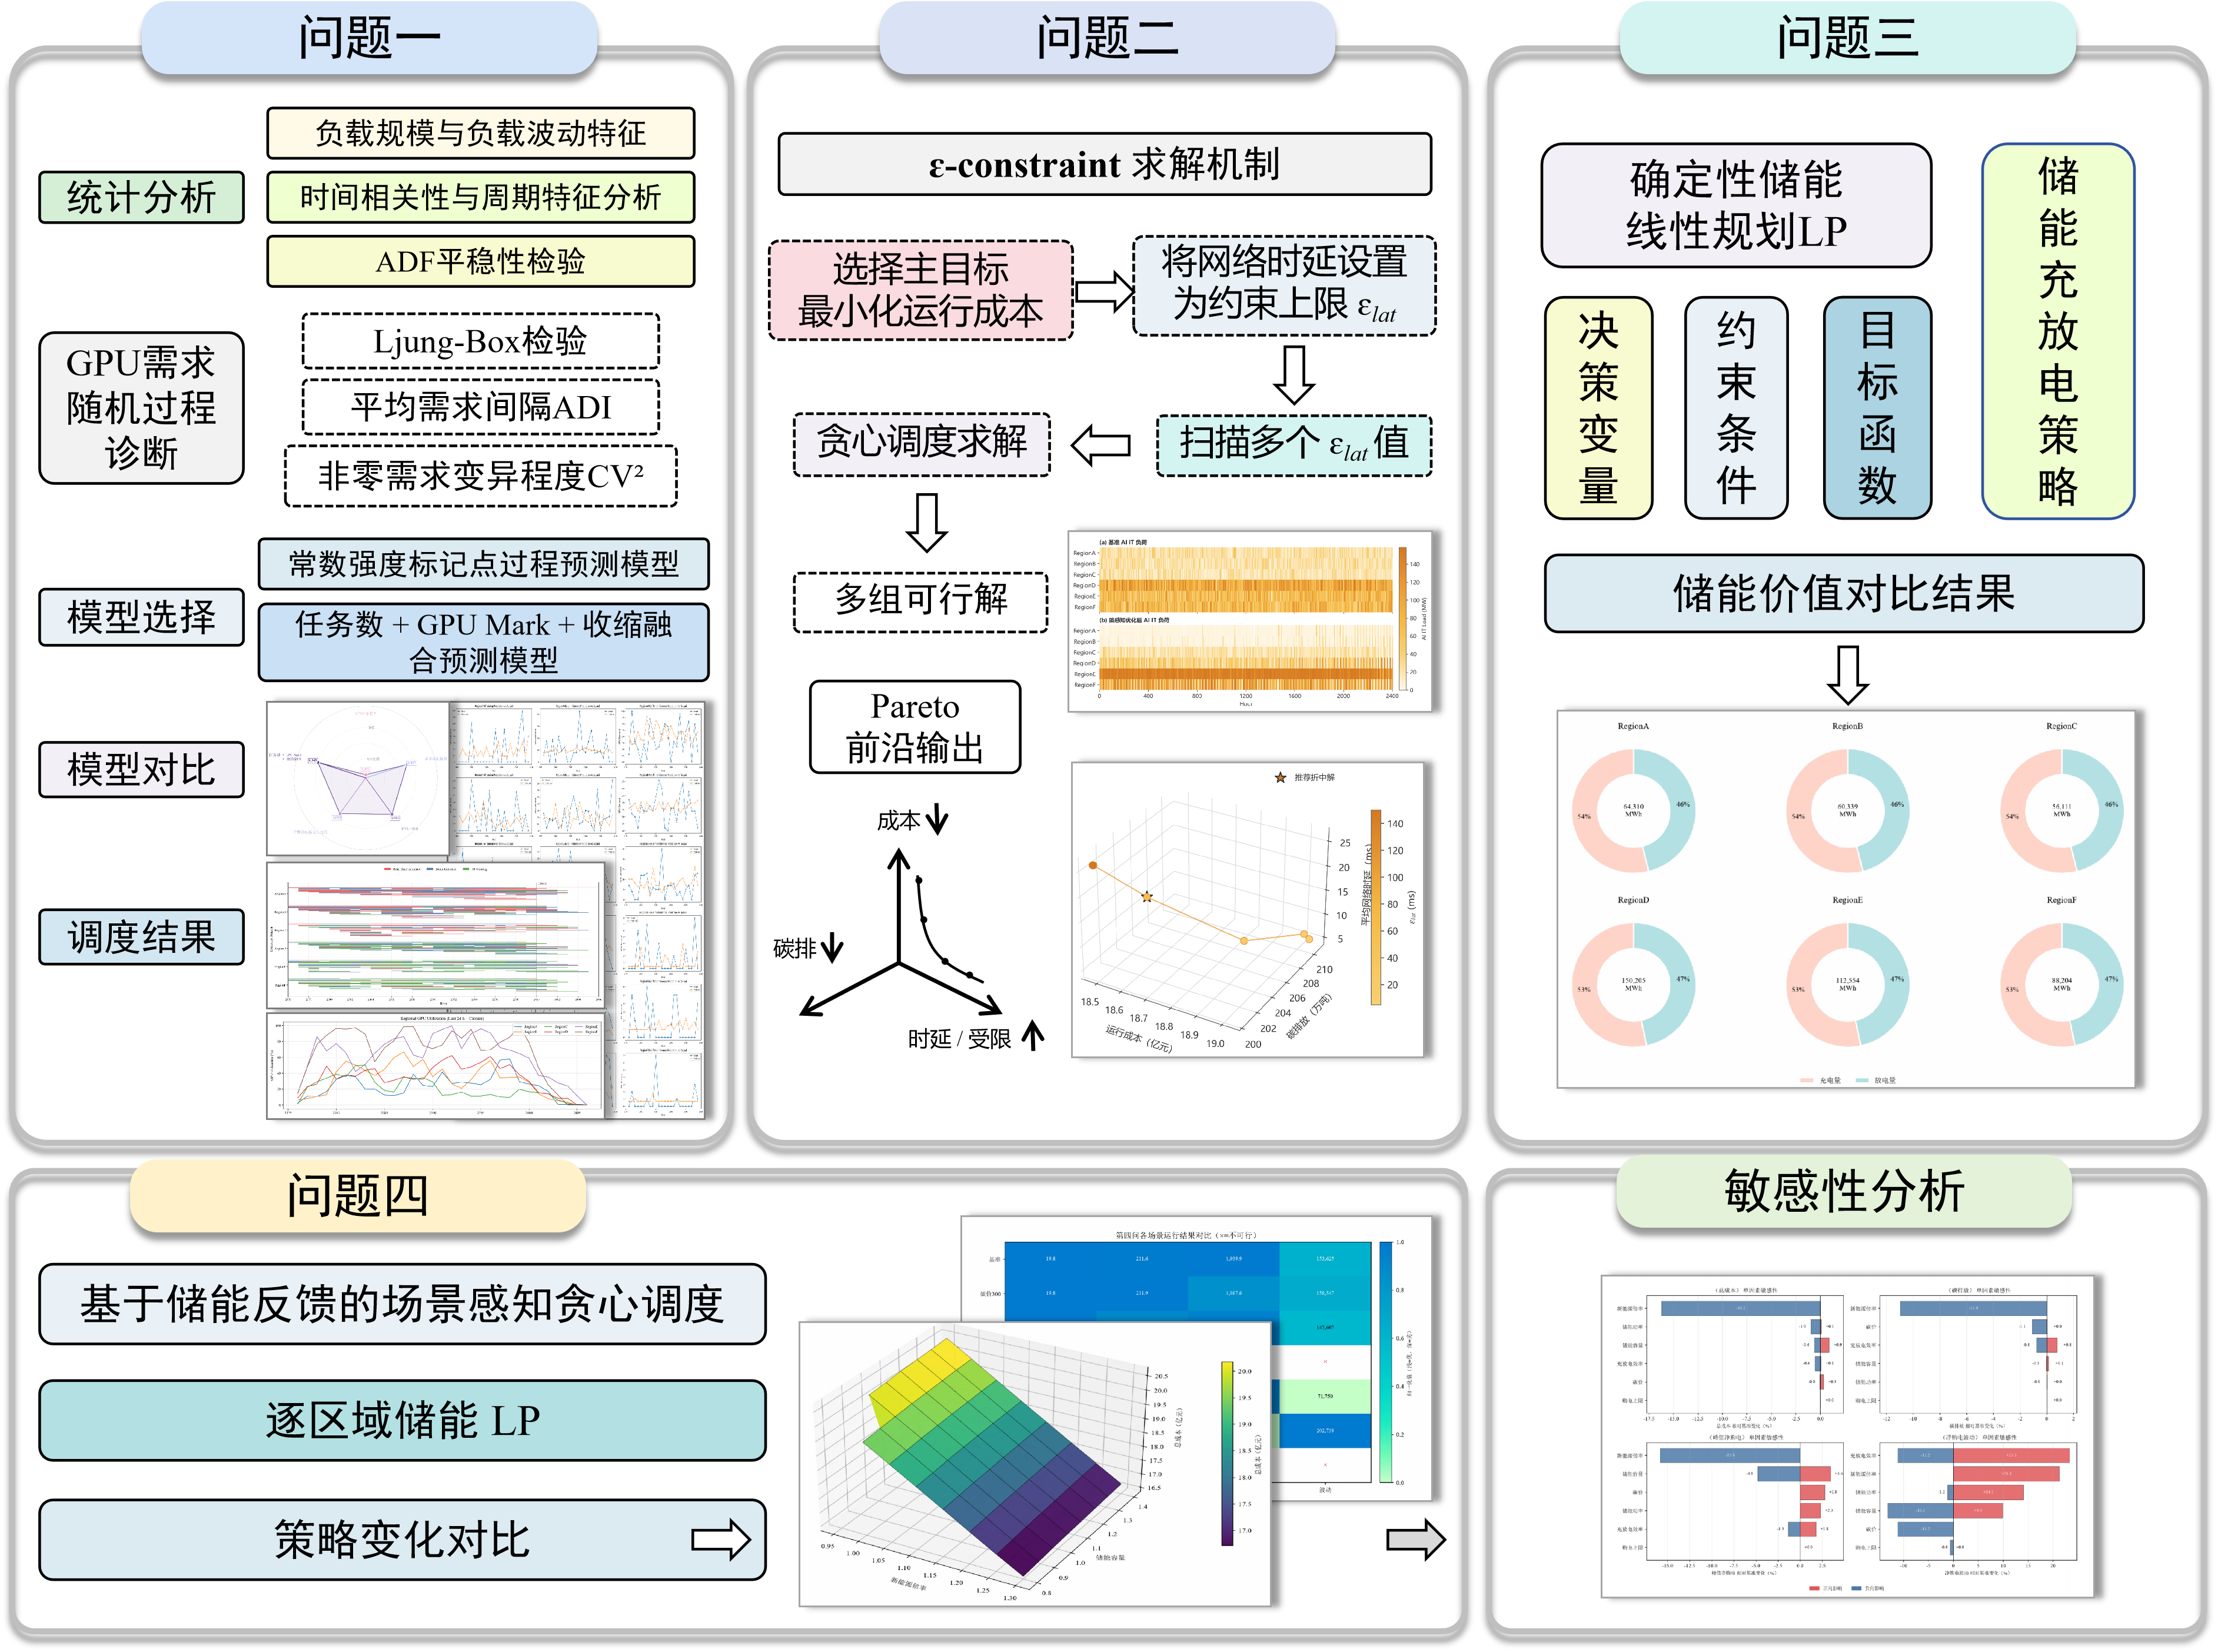
\includegraphics[width=1\textwidth]{figures/总技术路线图.png}
\caption{总技术路线图}
\end{figure}

\section{问题假设}

（1）\textbf{输入与物理系统假设}：赛题给出的电价、碳强度、硬件、任务等输入数据视为准确，仅情景分析可修改参数，模型直接使用清洗后数据，不额外做插值补全与噪声处理。算力负荷相关参数、PUE为区域定值，GPU按小时校验资源占用，忽略硬件故障异常；电力区域内部自平衡，新能源消纳、购售电、弃电遵从赛题规则；储能充放电效率恒定，满足SOC约束，仿真终点储能SOC不低于初始水平，禁止同时充放电。

（2）\textbf{任务调度与时序网络假设}：任务不可抢占、不可拆分、不可中途迁移，迁移仅考虑给定单向时延，忽略迁移带宽、能耗成本；实时推理任务到达即本地启动。任务启停受自身时间参数和全局2406小时硬截止约束，运行时长规整为整数小时。网络时延仅由源‑执行区域配对决定，仅校验单向时延阈值，不考虑拥塞、抖动等扰动。

（3）\textbf{求解、预测与核算口径假设}：负载预测仅使用历史聚合算力数据，调度采用点预测，不专门建模极端尖峰；任务调度采用启发式贪心获取高质量可行解，储能使用确定性线性规划，多目标权重为主观偏好，不存在客观唯一最优。成本仅核算购售电收支，碳排放仅统计外购电力与储能损耗带来的排放，不计设备全生命周期、新能源隐含碳与运维折旧等开销。

\section{符号说明}

\begin{table}[H]\zihao{-5}
\centering
\caption{符号说明表}
\begin{tabularx}{\textwidth}{c>{\centering\arraybackslash}X}
\toprule
符号&说明\\
\midrule
$i,r,t,s$&分别表示任务、区域、运行小时和候选开工小时索引\\
$g_i$&任务$i$的等效GPU需求\\
$d_i$&任务$i$折算后的连续运行时长（h）\\
$\ell_t,b_t,s_t$&ETS的水平、趋势与季节分量\\
$\alpha,\beta,\gamma$&ETS水平、趋势与季节的平滑参数\\
$m$&ETS季节周期长度（24小时）\\
$\hat{y}_{t+h}$&未来$h$小时的需求预测值\\
$q$&Split Conformal预测区间的校准分位数\\
$x_{i,r,s}$&任务$i$是否在区域$r$、小时$s$开工的0-1决策变量\\
$L(\mathrm{src}_i,r)$&任务来源区域到执行区域$r$的单向网络时延（ms）\\
$P_g$&对应任务类型每等效GPU的平均IT功率（MW/GPU）\\
$AI_{r,t}$&区域$r$在$t$时刻由任务调度形成的AIIT负荷（MW）\\
$PUE_r$&区域$r$的能源使用效率\\
$G_{r,t}$&电网购电功率（MW）\\
$S_{r,t}$&新能源外送/售电功率（MW）\\
$C_{r,t},D_{r,t}$&储能充电功率与放电功率（MW）\\
$E_{r,t}$&储能时段末荷电状态SOC（MWh）\\
$\eta_c,\eta_d$&储能充电效率与放电效率\\
$p_{r,t}$&区域-小时购电价格（元/MWh）\\
$\lambda_{r,t}$&区域-小时电网碳强度（tCO$_2$/MWh）\\
$P_r$&区域$r$的最大净购电功率（MW）\\
$\Delta_{r,t}$&净购电相邻小时波动的线性化辅助变量\\
$\varepsilon_{lat}$&$\varepsilon$-constraint中允许的网络时延约束参数\\
\bottomrule
\end{tabularx}
\end{table}

\section{数据预处理}

检查$\mathrm{workload\_tasks}$中50000条任务的到达时刻、来源区域、任务类型、GPU需求、预计时长、最大时延与最晚完成时刻等关键字段，并将预计执行分钟数向上取整为连续执行小时：
\begin{equation}
d_i=\mathrm{ceil}(\mathrm{EstimatedDuration\_min}/60)
\end{equation}
以保证不可抢占任务完整占用小时级资源。问题一按“区域—任务类型—小时”聚合、无到达小时补0，得18条长度2400的GPU需求序列；问题二、四以实际任务逐条调度，结合$\mathrm{network\_latency}$构造迁移可行集，按power\_mapping将GPU占用转为AIIT功率，加$\mathrm{NonAI\_IT\_Load}$后乘PUE得设施负荷；问题三直接用赛题给定IT负荷。能源指标统一按“购电功率×碳强度”“购电成本−售电收益”及受限新能源消纳口径计算。

\section{问题一模型建立与求解}

\subsection{统计分析}

首先对AI工作负载数据进行时间序列化处理，将原始任务请求转换为区域-任务类型粒度下的GPU需求序列。在此基础上，从负载规模与波动特征、周期规律以及平稳性三个方面开展统计分析。其中，通过均值和分位数刻画不同任务的算力需求水平，通过变异系数分析负载不确定性，通过自相关分析挖掘日周期和周周期特征，并利用ADF检验判断序列平稳性\cite{barroso2019,hyndman2021}。最终得到不同任务类型和区域的负载特征，为后续GPU资源预测模型构建以及算力调度优化提供数据依据。

\subsubsection{负载规模与负载波动特征分析}

\begin{table}[H]\zihao{-5}
\centering
\caption{不同任务类型的算力需求规模分析}
\begin{tabularx}{\textwidth}{*{3}{>{\centering\arraybackslash} X}}
\toprule
AI 任务类型 & 平均 GPU 需求 & CV\\
\midrule
AI 训练任务 & 491.810&0.418\\
批量推理任务 & 94.190&0.402\\
实时推理任务 & 28.000&0.431\\
\bottomrule
\end{tabularx}
\end{table}

三类任务具有明显的算力层级差异：AI训练属于高算力消耗型任务，需要长期占用大量GPU资源；批量推理任务具有中等规模计算需求；实时推理任务虽然单次资源需求较低，但由于具有在线响应要求，对调度实时性要求更高\cite{barroso2019}。

进一步观察最大值可以发现，AI训练任务峰值需求远高于其他任务，说明训练任务容易形成较大的瞬时算力压力。因此，在后续算力调度过程中，需要优先考虑训练任务的资源预留和峰值容量保障。

实时推理任务受用户访问请求影响较大，请求数量随时间变化明显，因此容易出现突发负载；AI训练任务虽然绝对波动最大，但由于基础需求规模较高，其相对波动程度并未显著超过其他任务。因此，对于实时推理任务，应重点关注瞬时变化和快速响应；对于AI训练任务，应重点关注长期资源规划和峰值容量配置。

\begin{figure}[H]
\centering
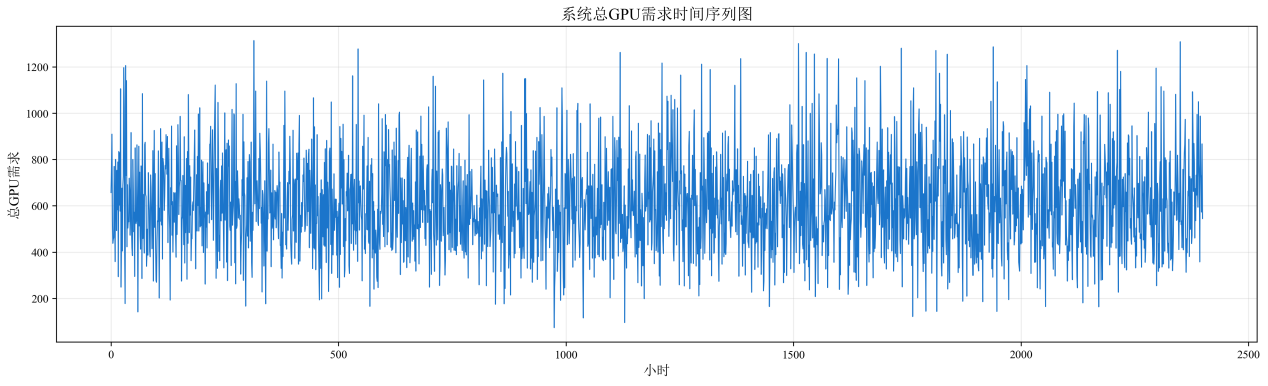
\includegraphics[width=1\textwidth]{figures/系统总GPU需求时间序列图.png}
\caption{系统总GPU需求时间序列图}
\end{figure}

由系统总GPU需求时间序列图可知，整体负载主要围绕相对稳定的水平上下波动，未表现出持续上升或下降趋势。同时，序列中存在较频繁的随机峰值和谷值，但未观察到明显的固定周期结构。这表明系统GPU需求具有较强的随机波动特征，而长期趋势相对稳定。后续进一步通过自相关分析和ADF检验，对其周期性和平稳性进行定量验证。

\subsubsection{时间相关性与周期特征分析}

为了判断GPU需求是否具有时间规律，对负载序列进行了不同时间尺度的自相关分析。

\begin{figure}[H]
\centering
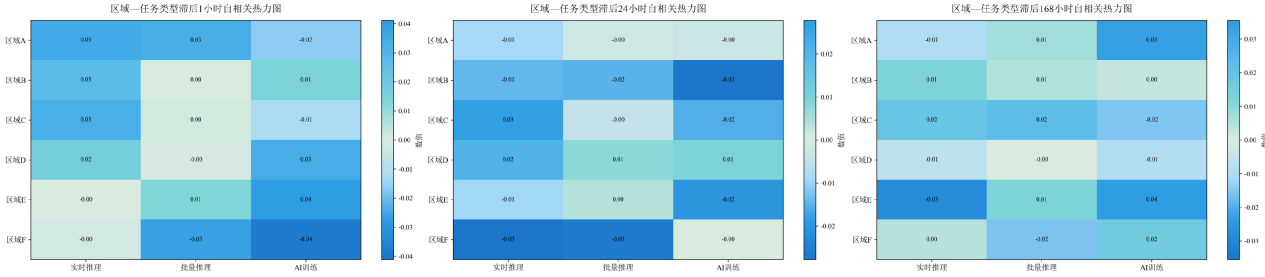
\includegraphics[width=1\textwidth]{figures/各区域—任务类型序列在不同滞后下的自相关系数.png}
\caption{各区域—任务类型序列在不同滞后下的自相关系数}
\end{figure}

分别计算各区域-任务类型GPU需求序列在滞后1小时、24小时和168小时下的自相关系数\cite{hyndman2021}。结果显示，各组合的相关系数均集中在 -0.04～0.04 附近，整体接近0。说明负载序列的短期连续性较弱，同时不存在明显的日周期和周周期特征。由此可见，GPU需求变化主要表现为随机波动，固定时间规律较弱，后续预测模型不宜过度依赖简单的季节周期结构。

\subsubsection{ADF平稳性检验}

为判断GPU需求序列是否平稳，采用ADF（Augmented Dickey-Fuller）检验，其回归形式为：
\begin{equation}
\Delta y_t=\alpha+\beta t+\gamma y_{t-1}
+\sum_{i=1}^{p}\delta_i\Delta y_{t-i}+\varepsilon_t
\end{equation}
其中$\Delta y_t$为一阶差分，$p$为滞后阶数；$H_0:\gamma=0$表示存在单位根、非平稳，$H_1:\gamma<0$表示平稳。以显著性水平$0.050$为判据（$p<0.050$拒绝$H_0$），18条序列均通过ADF检验，平稳性较好，可直接建模，无需差分。

\subsection{GPU需求随机过程诊断}

前述分析表明GPU需求整体平稳但周期性较弱，因此进一步从随机过程角度分析其到达机制与间歇性特征。首先利用Ljung-Box检验判断序列是否存在显著时间相关性；随后计算平均需求间隔ADI与非零需求变异程度$\mathrm{CV}^2$\cite{syntetos2005}：

\begin{equation}
ADI=\frac{N}{n_{+}},\qquad
CV^2=\left(\frac{\sigma_{+}}{\mu_{+}}\right)^2
\end{equation}

其中，$N$ 为总时段数，$n_{+}$ 为非零需求时段数。依据 $ADI=1.32$、$CV^2=0.49$ 将需求划分为平滑型、波动型、间歇型和突发块状型\cite{syntetos2005}。

进一步统计每小时任务到达次数，并采用离散指数

\begin{equation}
D=\frac{\operatorname{Var}(N_t)}{E(N_t)}
\end{equation}

刻画到达过程的随机性与聚集程度，同时分析非零需求间隔。最终综合时间相关性、间歇性和到达离散程度，判断负载的可预测性，并为后续预测模型选择提供依据。



诊断结果表明，18个“区域—任务类型”组合中，多数被划分为间歇型需求，仅部分组合属于平滑型，且所有组合的 $CV^2<0.49$，说明非零需求幅度本身并不存在剧烈波动，主要不确定性来自需求出现时点的间歇性。

Ljung-Box检验显示，除区域B的AI训练外，其余序列基本呈现白噪声特征，说明历史负载的线性时间依赖较弱。与此同时，各组合任务到达过程的离散指数均接近1：

\begin{equation}
D=\frac{\operatorname{Var}(N_t)}{E(N_t)}\approx1
\end{equation}

表明任务到达整体接近Poisson型随机到达过程，未出现明显过度离散。
进一步看非零需求间隔，区域D、E、F的实时推理平均间隔较大，最大间隔分别达到31、16和36小时，间歇性最为明显。综合来看，GPU负载主要表现为随机到达、弱相关、局部间歇的特征，因此后续预测不宜单纯依赖传统平滑或周期模型，应重点刻画任务到达概率及非零需求规模。

\subsection{模型选择}

\subsubsection{常数强度标记点过程预测模型}

前述分析表明，GPU需求整体具有平稳、弱自相关、随机到达和局部间歇特征，因此本文不再采用强周期性的传统时间序列模型，选用常数强度标记点过程预测模型。针对每个 Region × TaskType，将 GPU 需求序列建模为标记点过程。假设任务到达服从常数强度泊松过程：

\begin{equation}
N(t)\sim Poisson(\lambda t)
\end{equation}

其中 $\lambda$ 表示任务发生强度。利用训练集估计：

\begin{equation}
\hat{\lambda}=\frac{\sum_{t=1}^{T}I(Y_t>0)}{T}
\end{equation}

表示单位时间内任务出现概率。

对于发生任务的时间点，将 GPU 需求作为标记值（mark），计算平均资源消耗：

\begin{equation}
\hat{m}=E(Y_t|Y_t>0)
\end{equation}

则未来 GPU 需求期望为：

\begin{equation}
\hat{Y}_{t+h}=\hat{\lambda}\hat{m},\quad h=1,\dots,24
\end{equation}

即使用历史数据估计出的固定事件强度和平均标记值，生成未来 24 小时预测序列。

模型验证采用归一化误差：

\begin{equation}
RMSE=\sqrt{\frac{1}{H}\sum_{h=1}^{H}(Y_h-\hat{Y}_h)^2}
\end{equation}

\begin{equation}
RMSE/\sigma=\frac{RMSE}{\sigma(Y)}
\end{equation}

最终计算所有 Region × TaskType 序列的平均 $RMSE/\sigma$ 作为模型性能指标。

从验证结果看，常数强度标记点过程的平均 $RMSE/\sigma$ 约为 $1.019$，整体预测效果仍不理想。这说明不同区域、不同任务类型下的任务到达频率与单次 GPU 消耗存在明显异质性，采用统一的常数强度难以充分刻画其差异。因此，后续进一步对任务负载进行分层建模，将总 GPU 需求拆分为“任务数”和“GPU mark”两个部分分别预测，并结合收缩融合机制提高预测稳定性与泛化能力。

\subsubsection{任务数 + GPU Mark + 收缩融合预测模型}

为进一步刻画不同区域、任务类型下负载强度与单任务资源需求的差异，将 GPU 总需求理解为“任务到达数量”与“单任务 GPU Mark”的共同作用，并在小时级总 GPU 序列上进行分层预测。针对每个 `Region × TaskType`，分别构造近期均值、周期滞后、同小时多日均值/中位数以及周周期均值等多尺度候选预测器，以捕捉短期波动和日、周周期特征。

为降低局部预测的随机波动，引入收缩融合机制，将候选模型预测值与训练集长期均值进行加权：

\begin{equation}
\hat{Y}_t=\alpha \hat{Y}^{model}*t+(1-\alpha)\bar{Y}*{train}
\end{equation}

其中 $\alpha\in[0,1]$，通过验证集搜索使 $RMSE/\sigma$ 最小，并为不同区域和任务类型分别确定最优模型及收缩系数。

\begin{figure}[H]
\centering
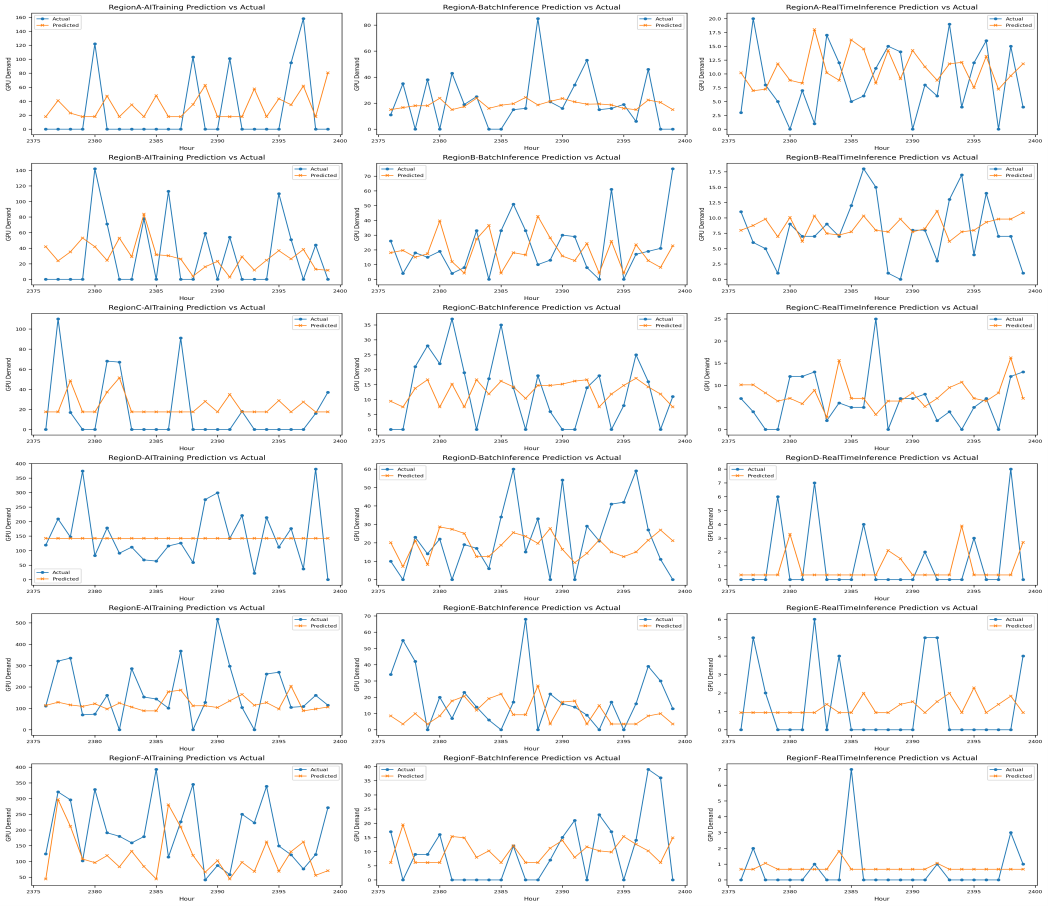
\includegraphics[width=1\textwidth]{figures/18条“区域—任务类型”序列ETS预测值与实际值对比.png}
\caption{18条“区域—任务类型”序列ETS预测值与实际值对比}
\end{figure}

结果表明，18 个序列的平均验证集 $RMSE/\sigma$ 降至 0.9490，明显低于常数强度模型的约 1.019；其中最优值达到 0.8087，且绝大多数序列均低于 1，说明模型具有较好的预测精度和稳定性。因此，最终选用该多尺度预测与收缩融合模型进行未来 24 小时 GPU 需求预测。

\subsection{模型对比}

为进一步检验模型的预测性能，在前述方法基础上引入 ETS/SES 指数平滑模型进行对比。ETS/SES通过对历史观测赋予递减权重，使近期数据对预测结果具有更大影响，能够较好地描述序列的局部水平变化\cite{hyndman2021}。对于简单指数平滑，其基本更新形式为：

\begin{equation}
\ell_t=\alpha y_t+(1-\alpha)\ell_{t-1},
\end{equation}

并以当前平滑水平作为未来预测：

\begin{equation}
\hat{y}_{t+h}=\ell_t.
\end{equation}

采用统一的验证集 $RMSE/\sigma$ 指标进行比较，结果表明：季节朴素模型、季节基准模型、ETS/SES 和常数强度标记点过程的平均验证集 $RMSE/\sigma$ 分别为 1.472、1.027、1.011419 和 1.019，而“任务数 + GPU Mark + 收缩融合”模型取得 0.949049 的最低值。

\begin{figure}[H]
\centering
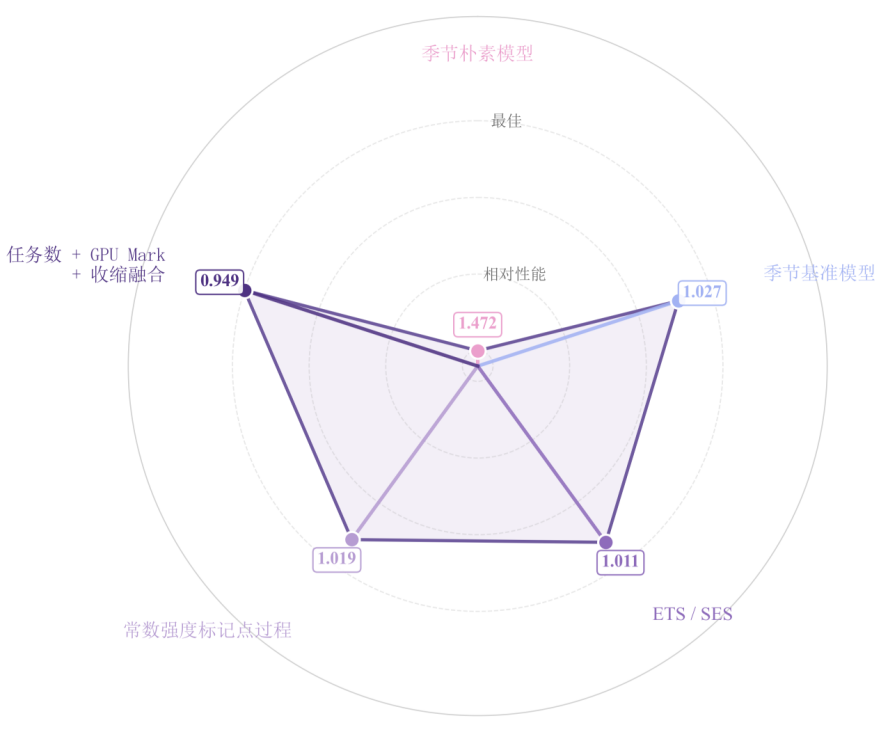
\includegraphics[width=1\textwidth]{figures/各模型测试集预测性能对比.png}
\caption{各模型测试集预测性能对比}
\end{figure}

可以看出，ETS/SES 相较于简单季节基准和常数强度模型已有一定改善，但仍未能充分刻画不同区域和任务类型下任务到达数量与单任务 GPU 消耗的差异。相比之下，“任务数 + GPU mark + 收缩融合”通过分别预测任务数量与 GPU 标记，并利用收缩机制降低短期波动和极端值带来的不稳定性，取得了所有候选模型中最小的验证误差。因此，最终选用该模型作为未来 GPU 需求的预测模型。

\subsection{调度结果}

将第 2376—2399 小时实际到达任务按到达时刻排序，实时任务到达即开工且优先固定在来源区域；批量推理和 AI 训练任务在满足网络时延、GPU 容量和最晚完成时限的候选区域中，优先来源区域，再按容量余量寻找可行开工时段。任务运行期间连续占用 GPU，任何任务均不可拆分或中途迁移。
最终共调度 538 个实际任务，末端任务均在 2400—2405 小时完成，2406 小时不安排任务；程序对每个区域—小时执行容量检查，未发现 GPU 容量越限。调度结构表现为实时推理主要留在东部来源区域，批量推理在容量紧张时向 D/E/F 扩展，AI 训练更充分利用 RegionD 的大规模可调度 GPU。

\begin{figure}[H]
\centering
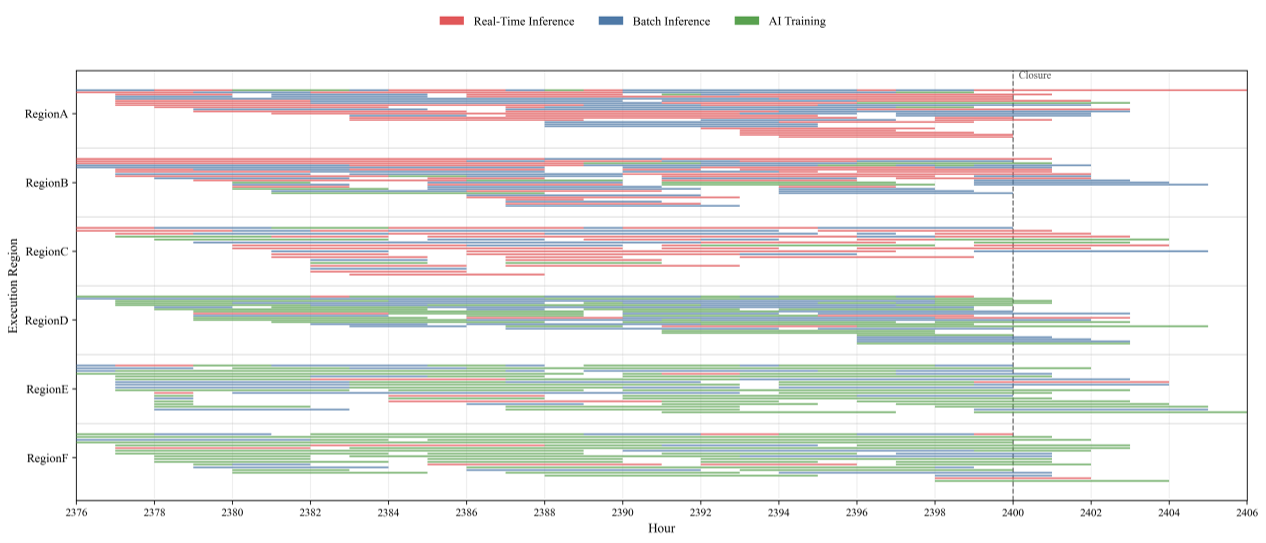
\includegraphics[width=1\textwidth]{figures/第2376—2406小时基础任务调度甘特图.png}
\caption{第2376—2406小时基础任务调度甘特图}
\end{figure}

\begin{figure}[H]
\centering
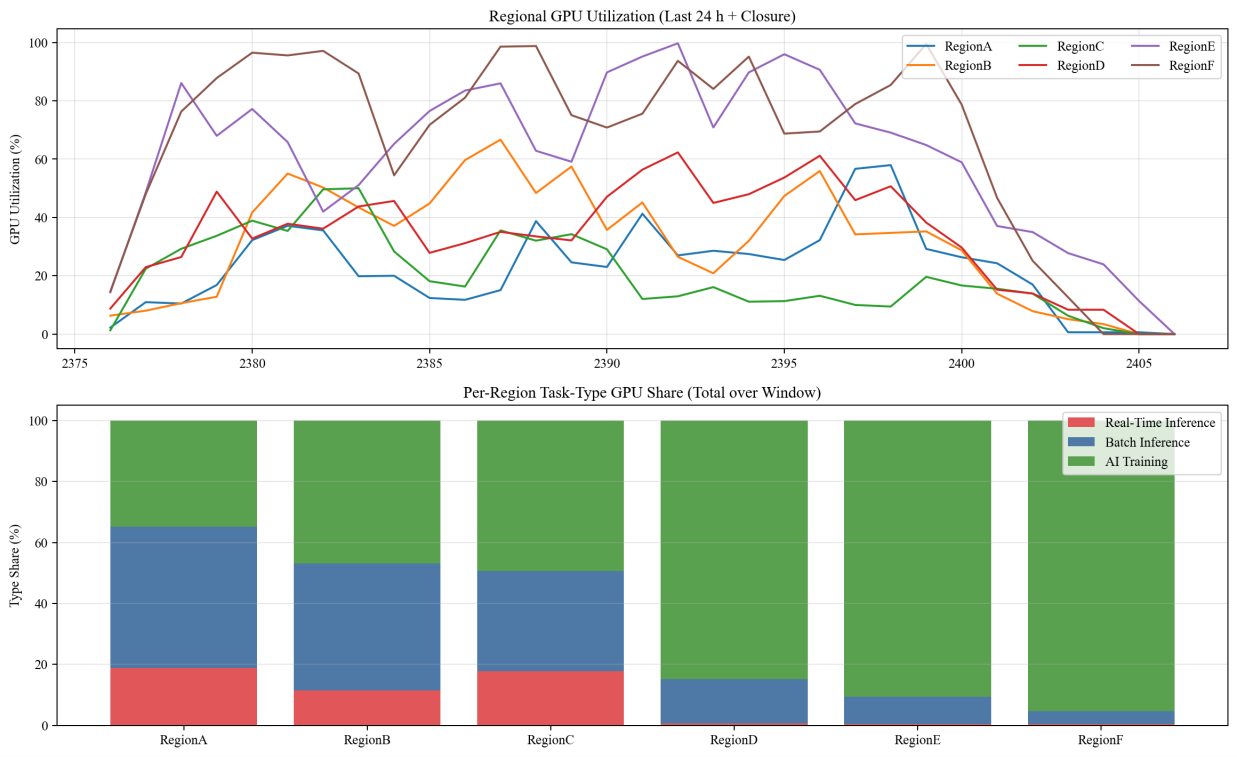
\includegraphics[width=1\textwidth]{figures/第2376—2406小时各区域GPU利用率与任务类型占比.png}
\caption{第2376—2406小时各区域GPU利用率与任务类型占比}
\end{figure}

图中展示了基础调度方案下六个区域在最后 24 小时及收尾时域内的 GPU 利用情况。上图显示各区域利用率随任务到达和延后调度动态变化，并在 2400–2405 小时逐步下降，符合末端任务结清要求。下图反映不同区域三类任务的 GPU 占比，其中 RegionD–F 以 AI 训练任务为主，体现了弹性任务向算力资源较充裕区域调度的特征；RegionA–C 中推理任务占比较高，更符合东部高负荷、低时延业务需求的区域定位。

\section{问题二模型建立与求解}

对于问题二，以第0–2399小时实际到达任务及对应逐时电力参数为输入，以任务迁移目的地与开工时段为决策变量，在GPU容量、IT/设施功率、网络时延、完成时限和购售电边界约束下，对运行成本、碳排放、网络时延与新能源利用率进行协同权衡\cite{radovanovic2023,xiang2026}。针对5万条任务和2400小时主时域，采用任务级贪心列表调度构造可行解，并通过$\varepsilon$-constraint 扫描得到不同网络时延约束下的非支配解集\cite{mavrotas2009}。

\subsection{基于成本—碳—时延的贪心调度}

实时推理任务固定在来源区域并于到达时刻立即开工；批量推理与AI训练任务允许延迟和跨区域迁移\cite{radovanovic2023}。对每个弹性任务，首先依据任务自身MaxLatency、LatestFinishHour以及2406终止边界筛选可行区域与时窗，再逐一检查GPU容量、IT功率、设施功率和MaxGridImport硬约束，最后在可行候选中按综合得分选择执行方案。
\begin{equation}
\mathrm{score}(r,s)=w_{\mathrm{cost}}\,\tilde{C}(r,s)+w_{\mathrm{carbon}}\,\tilde{E}(r,s)+w_{\mathrm{lat}}\,\tilde{L}(\mathrm{src},r)
\end{equation}
在最终推荐的$\varepsilon_{\mathrm{lat}}=60$ ms 情景下，5万个任务全部获得可行调度：跨区域迁移26,300个，迁移率为52.60\%。迁移主要发生在批量推理与AI训练任务中。

\begin{figure}[H]
\centering
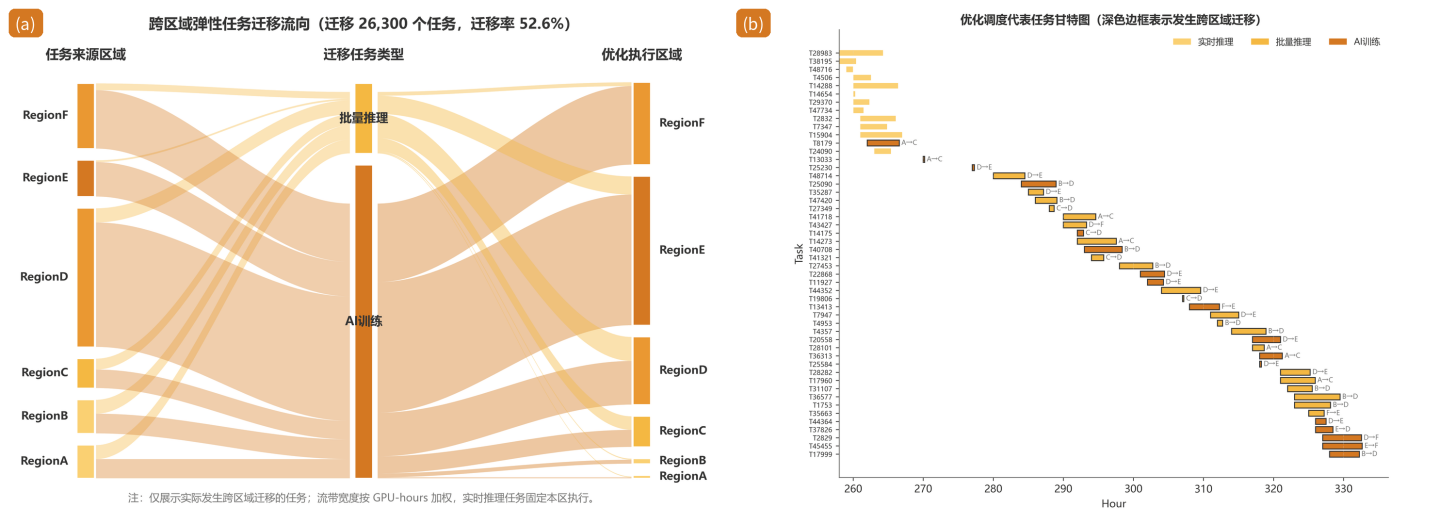
\includegraphics[width=1\textwidth]{figures/跨区域弹性任务迁移流向.png}
\caption{跨区域弹性任务迁移流向}
\end{figure}

图中展示了碳感知调度下任务迁移与执行行为。可以看出，跨区域迁移主要集中在批量推理和AI训练任务，实时推理任务基本保持本区执行；同时，甘特图表明部分弹性任务通过延迟开工和跨区域迁移重新分配到更合适的时段与区域，从而实现算力负荷的时空重构。

\subsection{多目标 $\varepsilon$-constraint 求解框架}

\subsubsection{决策变量与负荷映射}

定义二元变量$x_{i,r,s}\in\{0,1\}$，表示任务$i$是否在区域$r$的第$s$小时开工；该变量同时决定任务迁移目的地与开工时段。由任务调度唯一确定区域—小时AI IT负荷：
\begin{equation}
\mathrm{AI\_IT\_Load}(r,t)=\sum_i \mathrm{GPU\_Demand}_i\,\mathrm{Overlap}(i,r,t)\,\mathrm{GPU\_Power}(\mathrm{TaskType}_i)
\end{equation}
\subsubsection{目标函数与评价指标}

以运行成本为 $\varepsilon$-constraint 框架中的主优化目标，并同步评价碳排放、网络时延、新能源利用率与区域峰值净购电。
\begin{equation}
\mathrm{Cost}=\sum_{r,t}\left[\mathrm{GridPurchase}_{r,t}\,p_{r,t}-\mathrm{GridSell}_{r,t}\,p^{\mathrm{sell}}_{r,t}\right]
\end{equation}
\begin{equation}
\mathrm{Carbon}=\sum_{r,t}\mathrm{GridPurchase}_{r,t}\,\lambda_{r,t}
\end{equation}
\begin{equation}
\mathrm{Latency}=\sum_i L(\mathrm{src}_i,r_i)
\end{equation}
\begin{equation}
\mathrm{Util}=(\text{直接消纳}+\text{外送})/(\text{可用新能源})\times100\%
\end{equation}
\begin{equation}
\mathrm{Peak}=\sum_r\max_t\left[\mathrm{GridPurchase}_{r,t}-\mathrm{GridSell}_{r,t}\right]
\end{equation}
\subsubsection{约束条件}

（1）调度方案必须同时满足：

（2）区域小时级GPU占用不超过$\mathrm{Available\_GPU}$；

（3）NonAI+AI IT负荷不超过$\mathrm{MaxIT}-\mathrm{Power}_{\mathrm{MW}}$\allowbreak，设施负荷不超过$\mathrm{MaxFacility}-\mathrm{Power}_{\mathrm{MW}}$\allowbreak；

（4）任务跨区时延不超过$\mathrm{MaxLatency\_ms}$；

（5）任务在LatestFinishHour与时点2406之前完成，实时任务到达即开工；

（6）任务不可抢占、不可拆分或中途迁移；$\mathrm{GridPurchase}\le\mathrm{MaxGridImport}$，$\mathrm{GridSell}\le\mathrm{SellLimit}$。

最终推荐方案的统一验算表明上述硬约束全部通过。最大IT功率与设施功率的数值残差仅为6.94e-07 MW和9.37e-07 MW，均属浮点计算误差量级；GPU容量、最大购电、任务网络时延、2406完成边界及实时任务开工约束的违反量均为0。

\subsubsection{Pareto 前沿与折中方案选择}

采用 $\varepsilon$-constraint 法\cite{mavrotas2009}，将网络时延设置为硬约束上限 $\varepsilon_{\text{lat}}$，扫描{5,15,25,40,60,80,150} ms。对每个阈值独立执行任务级贪心调度，并对成本—碳排—时延等目标进行非支配筛选。

\begin{figure}[H]
\centering
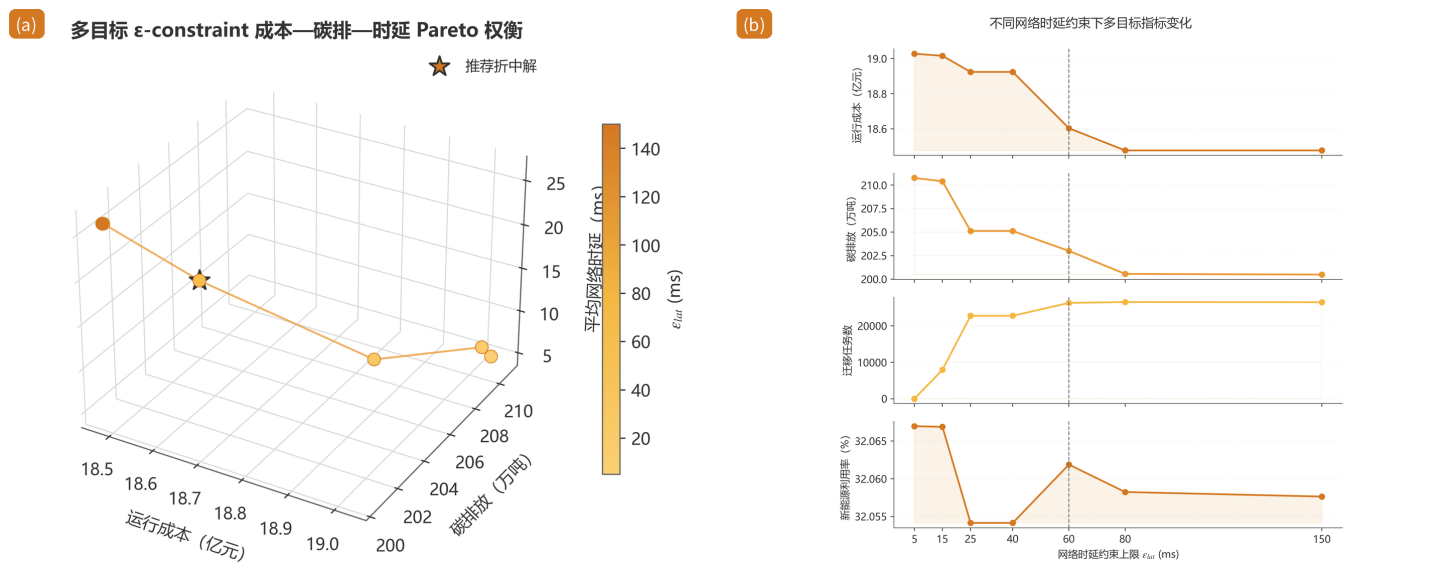
\includegraphics[width=1\textwidth]{figures/多目标epsilon-constraint 成本一碳排一时延Pareto权衡.png}
\caption{多目标 $\varepsilon$-constraint 成本—碳排—时延 Pareto 权衡}
\end{figure}

随着网络时延约束上限 $\varepsilon_{lat}$ 逐步放宽，可迁移任务获得更大的区域选择空间，运行成本和碳排放总体呈下降趋势，但平均网络时延和任务迁移规模随之增加。

其中，$\varepsilon_{lat}=60\,\mathrm{ms}$ 处于较明显的折中位置。相较于 $\varepsilon_{lat}=5\,\mathrm{ms}$ 的本区调度方案，运行成本由 19.028 亿元下降至 18.603 亿元，降低约 2.23\%；碳排放由 210.758 万吨下降至 203.002 万吨，降低约 3.68\%，而平均网络时延由 5.00 ms 增加至 18.32 ms。

当 $\varepsilon_{lat}$ 进一步由 $60\,\mathrm{ms}$ 放宽至 $80\,\mathrm{ms}$ 时，运行成本和碳排放仅获得有限的进一步改善，而平均网络时延明显增加，表现出较显著的边际收益递减特征。因此，综合考虑运行经济性、低碳性与服务时延，本文选取 $\varepsilon_{lat}=60\,\mathrm{ms}$ 作为最终推荐的折中调度方案。

\subsection{受限消纳口径与能源侧响应}

为避免因任务迁移而虚构新的新能源消纳通道，采用受限消纳口径\cite{bird2016}：区域—小时直接消纳量不超过附件基准$\mathrm{UsedRenewable\_MW}$对应的消纳能力，同时不超过当期$\mathrm{AvailableRenewable\_MW}$；富余新能源在SellLimit内优先外送，剩余部分计入弃电。
\begin{equation}
\mathrm{DirectRenewable}=\min(\mathrm{TotalLoad},\mathrm{UsedRenewable}_{\mathrm{baseline}},\mathrm{AvailableRenewable})
\end{equation}
\begin{equation}
\mathrm{GridSell}=\min(\max(\mathrm{AvailableRenewable}-\mathrm{DirectRenewable},0),\mathrm{SellLimit})
\end{equation}
\begin{equation}
\mathrm{GridPurchase}=\max(\mathrm{TotalLoad}-\mathrm{DirectRenewable},0)
\end{equation}
按附件基准状态与优化方案采用同一口径重算后，系统新能源利用率由31.06\%提高至32.06\%，绝对提高约1.00个百分点。RegionE由58.54\%提高至61.09\%，RegionF由56.06\%提高至59.23\%。这说明弹性任务确实向新能源资源更有利的时空位置重分配；但直接消纳能力与外送上限共同限制了系统层面的增幅，因此主要优化收益仍体现为成本和碳排的同步下降。

\begin{figure}[H]
\centering
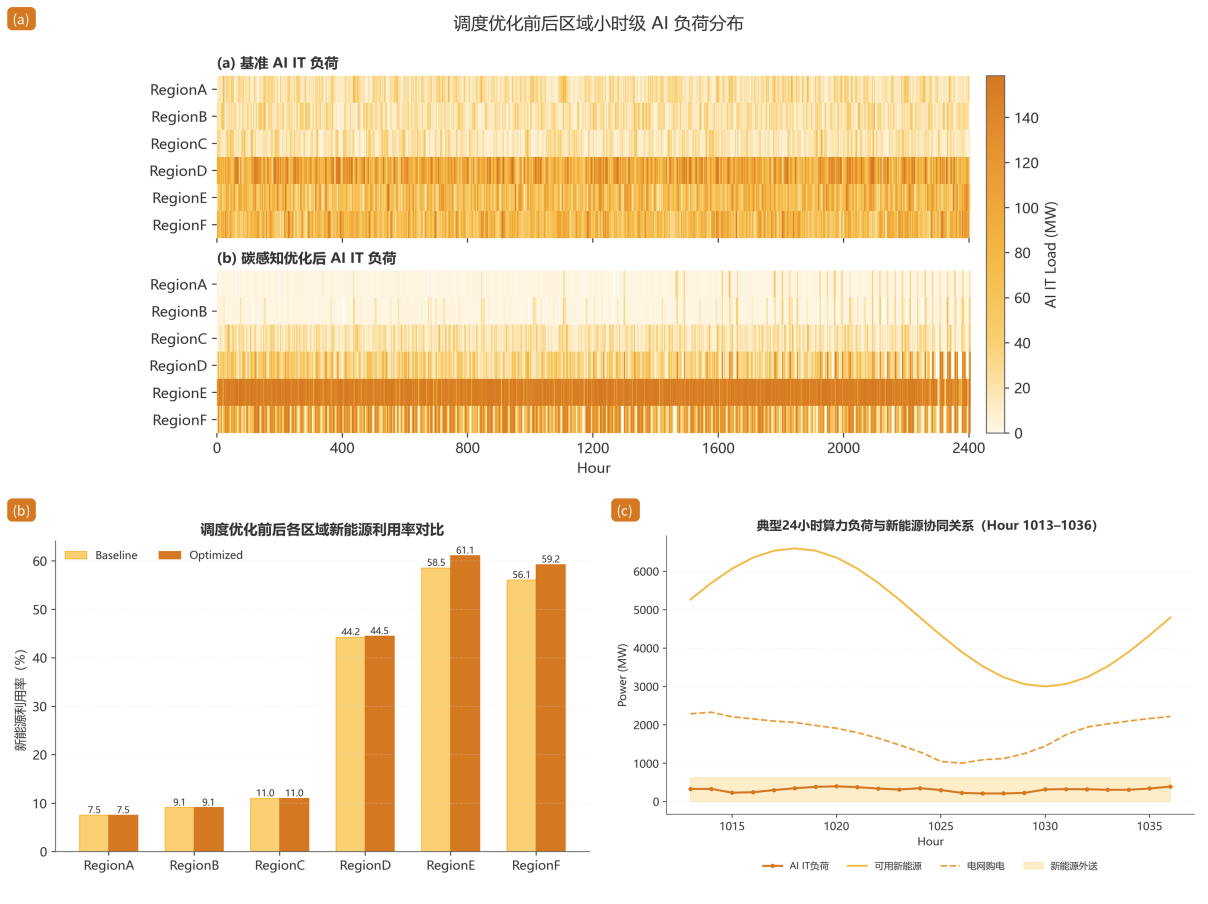
\includegraphics[width=1\textwidth]{figures/调度优化前后区域小时级AI负荷分布.png}
\caption{调度优化前后区域小时级AI负荷分布}
\end{figure}

图(a)展示优化前后区域AI IT负荷的重分布；图(b)展示各区域新能源利用率变化；图(c)展示典型24小时内AI负荷、新能源出力、电网购电与新能源外送的时序关系。三者共同说明模型通过“空间迁移+时间平移”重构算力负荷，同时保持购电边界和受限消纳边界可行。

综上，推荐的$\varepsilon=60$ ms 方案在全部任务可行和各项硬约束满足的前提下，相较$\varepsilon=5$ ms 本区调度基准实现成本下降2.23\%、碳排下降3.68\%，并将平均网络时延控制在18.32 ms。该方案在运行经济性、低碳性与服务时延之间形成较均衡的折中，可作为问题二的最终碳感知任务调度策略。

\section{问题三模型建立与求解}

问题三固定任务调度，仅以储能为连续决策对象：给定IT负荷乘各区域PUE得设施负荷，对六个区域分别构建0—2406小时LP。区域间无潮流耦合，逐区域求解可显著降维，也便于按区域解释充放电与削峰效果\cite{ding2022a,lawder2014}。

\subsection{确定性储能线性规划LP}

参数均已知，采用scipy.optimize.linprog（HiGHS）求解确定性LP；目标函数以无储能指标为尺度归一化，避免成本、碳排、峰值与波动因量纲不同而失衡。

\subsubsection{决策变量}

对区域$r$、小时$t$定义：$G_{r,t}$为购电功率，$S_{r,t}$为售电功率，$C_{r,t}$、$D_{r,t}$为储能充放电功率，$W_{r,t}$为弃电功率，$R^{use}_{r,t}$为直接消纳新能源功率，$E_{r,t}$为时段末SOC；另设$P_r$表示区域最大净购电功率，$\Delta_{r,t}$表示相邻小时净购电变化的绝对值辅助变量。

\subsubsection{目标函数}

归一化加权多目标：
\begin{equation}
\min\left[\frac{\mathrm{Cost}}{C_0}+\frac{W_1\cdot\mathrm{Carbon}}{\Lambda_0}+\frac{W_2\cdot{}P}{P_0}+\frac{W_3\cdot\sum\Delta}{V_0}\right]
\end{equation}
其中成本权重取1，$W_1=0.300$、$W_2=0.500$、$W_3=0.300$；$C_0,\Lambda_0,P_0,V_0$为无储能时的成本、碳排、峰值与波动基准，体现“经济性为基础、重点削峰并抑制波动”的偏好。

\subsubsection{约束条件}

负荷侧功率平衡为
\begin{equation}
G_t+R^{use}_t+D_t=\mathrm{TotalLoad}_t+C_t
\end{equation}
新能源侧直接消纳+储能充电+售电+弃电=可用新能源；SOC按
\begin{equation}
E_t=E_{t-1}+\eta_cC_t-D_t/\eta_d
\end{equation}
递推\cite{lawder2014}，初值$\mathrm{InitialSOC}$，且
\begin{equation}
\mathrm{MinSOC}\le{}E_t\le{}\mathrm{StorageCapacity}
\end{equation}
充放电、购售电均受附件上限约束。峰值以$P\ge{}G_t-S_t$线性化，波动以
\begin{equation}
\Delta_t\ge|(G_t-S_t)-(G_{t-1}-S_{t-1})|
\end{equation}
线性化，并要求$E_{2406}\ge\mathrm{InitialSOC}$。

\subsection{储能充放电策略}

最优策略总体呈“低价低碳充电、高价高峰放电、新能源富余优先充电”。东部A/B/C储能容量小，以峰谷套利与局部削峰为主；西部D/E/F储能规模大，还承担新能源时移与外送配合。以RegionD为例（900MWh、260MW），其尺度足以显著平抑西部算力中心净购电曲线。

\begin{figure}[H]
\centering
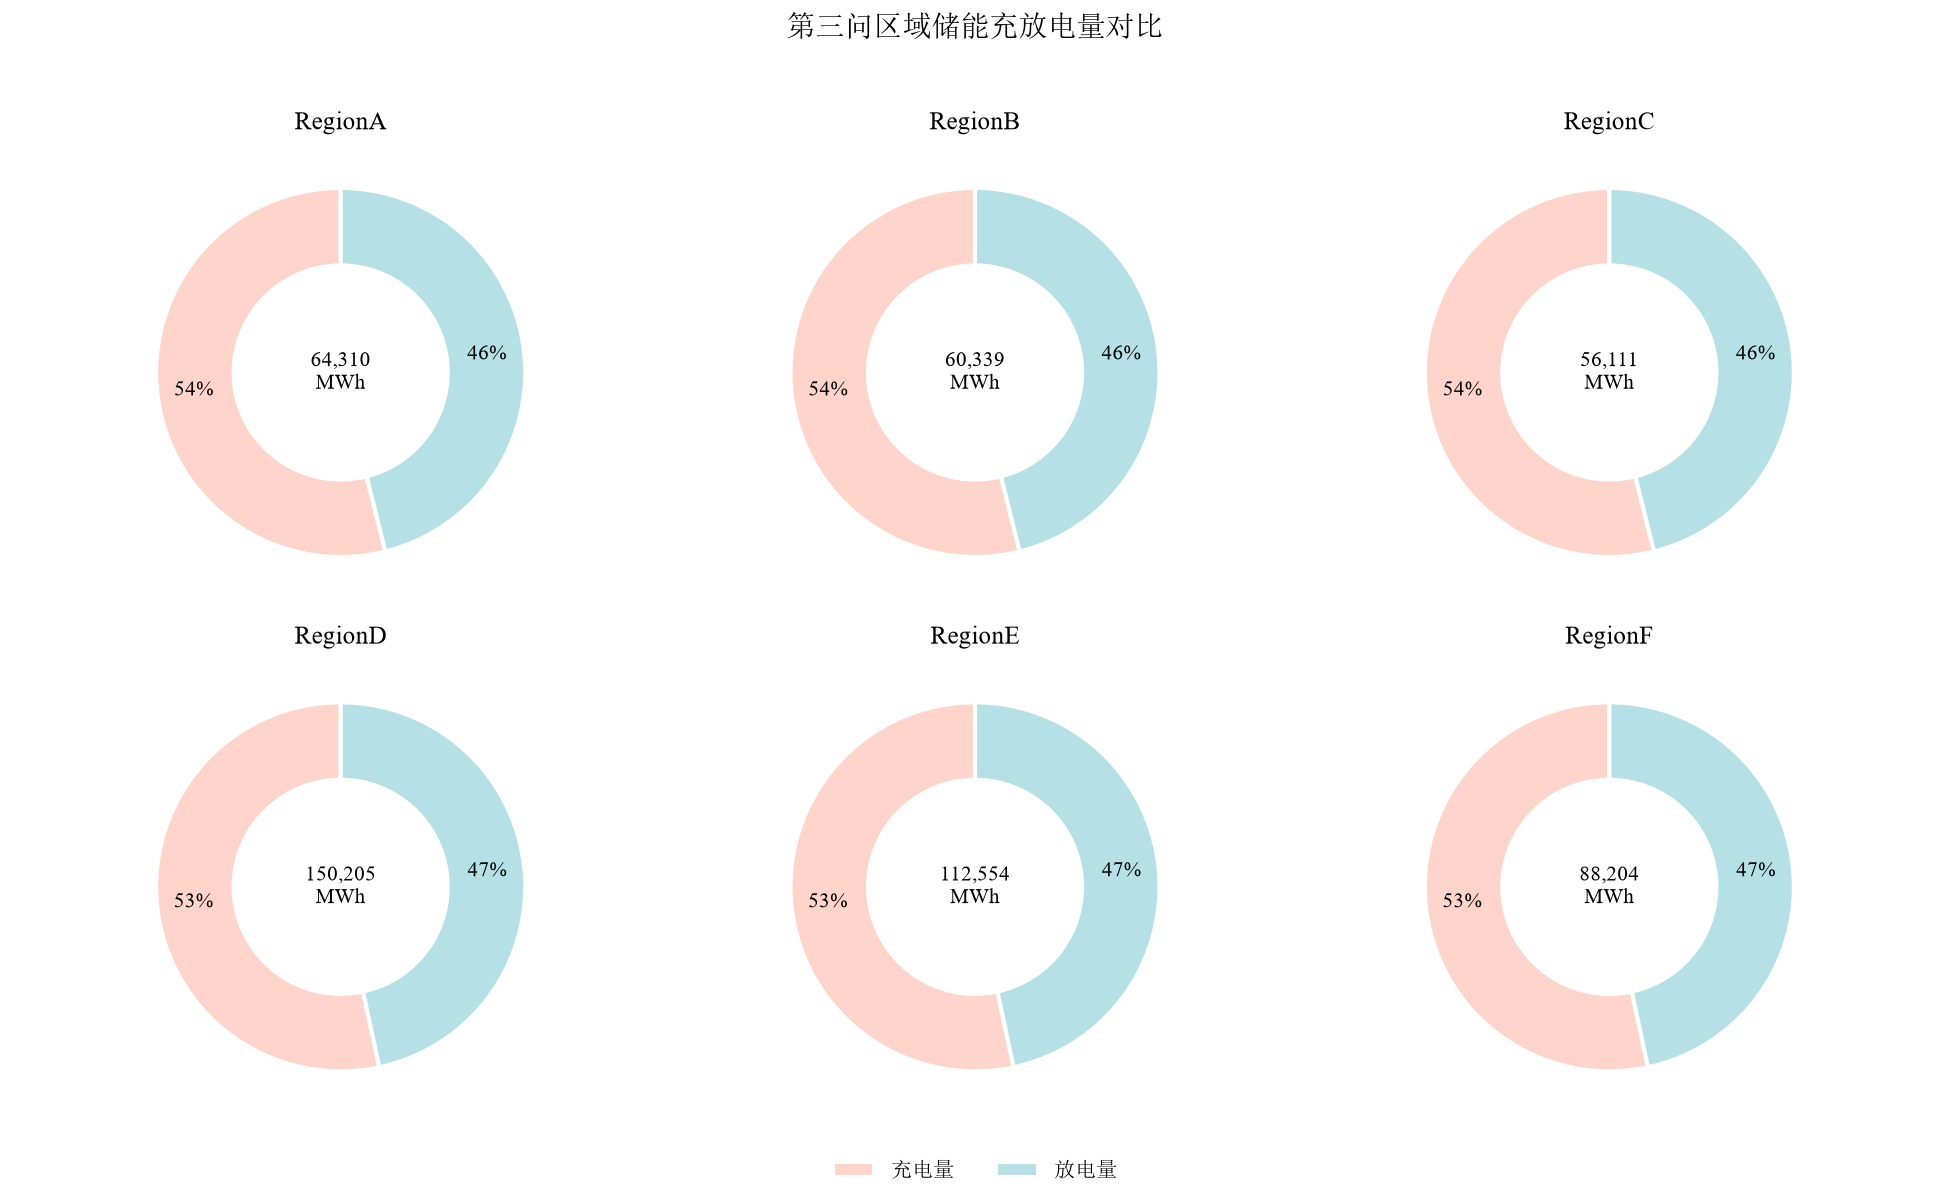
\includegraphics[width=0.85\textwidth]{figures/第三问区域储能充放电量对比.png}
\caption{第三问区域储能充放电量对比}
\end{figure}

由图可见，六个区域的储能充电量均略高于放电量，两者之差对应充放电损耗（约2.7\%），且各区域均无同时充放电现象，符合储能物理约束。东部A/B/C储能容量较小，充电量约3.0万~3.5万MWh，以峰谷套利与局部削峰为主；西部D/E/F储能规模较大，充电量达4.7万~8.0万MWh，其中RegionD充电量约8.0万MWh为最大，承担新能源富余电量的时移储存与高峰放电外送。充放电量的大小直接反映储能参与削峰填谷的深度，西部区域利用更充分，与前述西部大容量储能削峰与平抑效果尤为突出的结论相互印证。

\subsection{储能价值对比结果}

六区域合计：无储能成本23.880亿元，储能LP后降至20.130亿元（降15.690\%）；净购电峰值之和由2344.100降至1444.100MW（降38.390\%）；净购电总波动由250572降至62591（降75.020\%）。碳排由210.800万吨升至211.970万吨（+0.550\%），为明显削峰平滑所接受的少量充电损耗代价。

D/E/F削峰最突出，RegionE净购电峰值降至-15.100MW（峰值时段仍净外送），A/B/C峰值分别降至约463、436、426MW。附件基准成本更低，是因本文显式提高峰值与波动权重、偏向电网友好运行。

\begin{table}[H]\zihao{-5}
\centering
\caption{各区域储能价值对比}
\begin{tabularx}{\textwidth}{*{6}{>{\centering\arraybackslash}X}}
\toprule
区域&无储能成本/亿&储能LP成本/亿&LP碳排/万吨&LP峰值/MW&LP波动\\
\midrule
RegionA&6.440&6.610&59.470&462.900&22083\\
RegionB&5.910&6.050&53.110&436.300&20247\\
RegionC&5.630&5.760&49.400&425.500&19695\\
RegionD&2.650&1.420&28.330&134.500&357\\
RegionE&1.460&0.040&9.310&-15.100&157\\
RegionF&1.780&0.250&12.350&0.000&52\\
\bottomrule
\end{tabularx}
\end{table}

由表可知，加入储能后六区域总成本由23.880亿元降至20.130亿元（降15.690\%）。东部A/B/C储能以峰谷套利为主，成本小幅上升、峰值降幅有限；西部D/E/F受益于大容量储能，成本大幅下降，RegionE峰值降至-15.100MW实现净外送，削峰与平抑效果显著。碳排小幅上升0.550\%，为削峰填谷所接受的充放电损耗代价。

\section{问题四模型建立与求解}

问题四连接任务调度与储能运行并保持可计算规模：场景感知贪心按电价、碳价与时延形成任务时空分配，再储能LP，将储能后净购电高峰反馈进任务得分做一次协同迭代，使可延后计算主动避开储能难以消除的电网高峰\cite{radovanovic2023,huan2026,li2022}。

\subsection{基于储能反馈的场景感知贪心调度}

候选方案得分
\begin{equation}
\mathrm{score}(r,s)=P_{g}\,g_{i}\,p(r,s)+c_{CO_2}\cdot{}P_{g}\,g_{i}\,\lambda(r,s)+w_{lat}\,L(\mathrm{src}_i,r)+w_{net}\cdot{}\mathrm{nfrac}(r,s)
\end{equation}
其中$c_{CO_2}$取0、300或800元/吨表征碳约束强度，$\mathrm{nfrac}(r,s)$为储能后净购电占峰值的归一化比例；该反馈使弹性任务偏向净购电较低的区域—时段，在不改变实时任务SLA的前提下“算避储峰”。

\subsection{逐区域储能LP}

给定负荷后各区域沿用问题三LP。新能源场景以$\mathrm{renew\_mult}$同步缩放可用新能源与基准消纳能力（0.700、1.000、1.300）；电价场景含原始分时、固定均价与高波动三种。六区域LP求解后聚合成本、碳排、峰值与波动，净购电曲线用于下一轮反馈。

\begin{figure}[H]
\centering
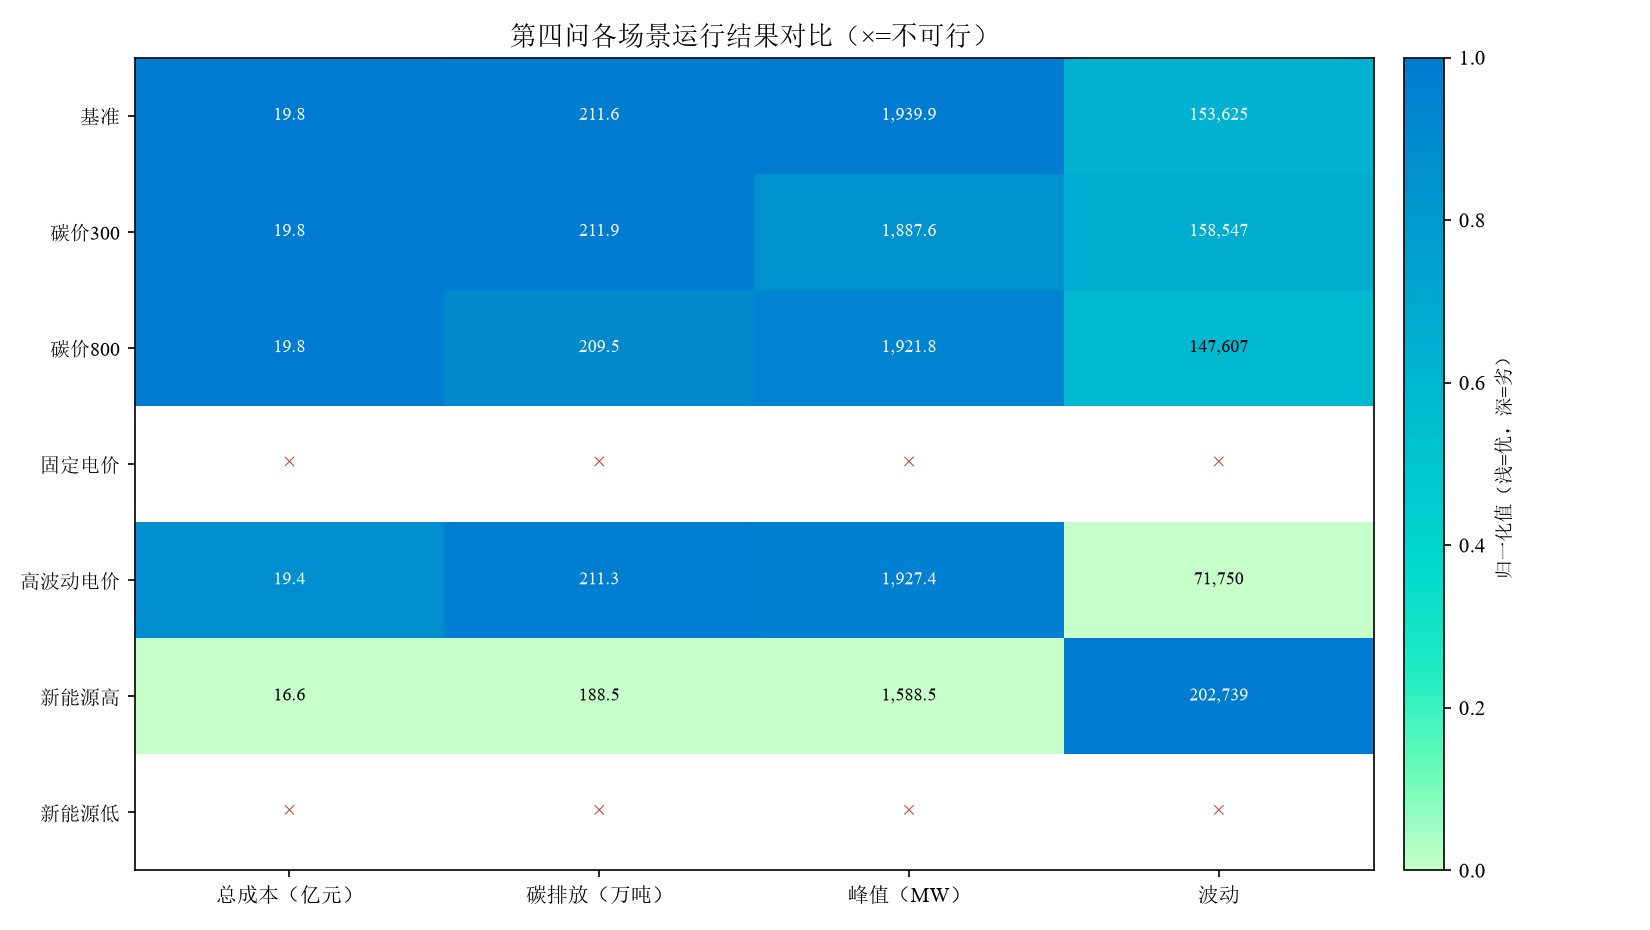
\includegraphics[width=1\textwidth]{figures/第四问各场景运行结果对比.png}
\caption{第四问各场景运行结果对比}
\end{figure}

热图对各指标在场景间作最小—最大归一化，浅色表示更优、深色表示更劣，×为不可行。基准、碳价300与碳价800三档碳约束下各指标差异有限：碳价升高主要使碳排由211.644万吨降至209.511万吨，成本与峰值基本持平，说明成本主导调度下碳价的边际减排作用有限。高波动电价放大移峰套利空间，波动降至7.175万、成本降至19.406亿元；新能源提高至1.300倍时成本最低（16.552亿元），碳排与峰值同步下降。固定电价与新能源0.700倍两场景因触发购电上限而不可行，直观揭示购电边界是弱分时、低新能源场景的核心瓶颈。

\subsection{策略变化对比}

调度层沿用第二问推荐的最优时延上限$\varepsilon=60$ms的碳感知方案，叠加逐区域储能LP与净购电反馈。分步方案（无碳调度+储能）成本19.798亿元、碳排211.645万吨、峰值1939.900MW；碳感知联合方案成本19.791亿元、碳排211.863万吨、峰值1887.600MW。与同调度无储能相比，储能把峰值由2498.900MW降24.500\%、波动由49.048万降至15.855万，代价是充放电损耗与更强削峰偏好推高成本（由18.870亿元升至19.791亿元）。

引入净购电反馈后，协同方案成本19.926亿元、碳排降至210.670万吨、峰值降至1805.000MW、波动降至12.758万，迁移数由26373增至26420，说明调度与储能层存在可利用的协同空间。

场景上：碳价升至800元/吨时碳排降至209.511万吨；固定电价削弱分时套利且受购电边界约束，储能LP不可行；高波动电价提供更多移峰机会，成本降至19.406亿元；新能源提高至1.300倍时成本16.552亿元、碳排188.535万吨。新能源降至0.700倍时，部分区域无储能净购电峰值超过MaxGridImport，储能LP不可行，购电边界成为低新能源场景的关键瓶颈。

\begin{figure}[H]
\centering
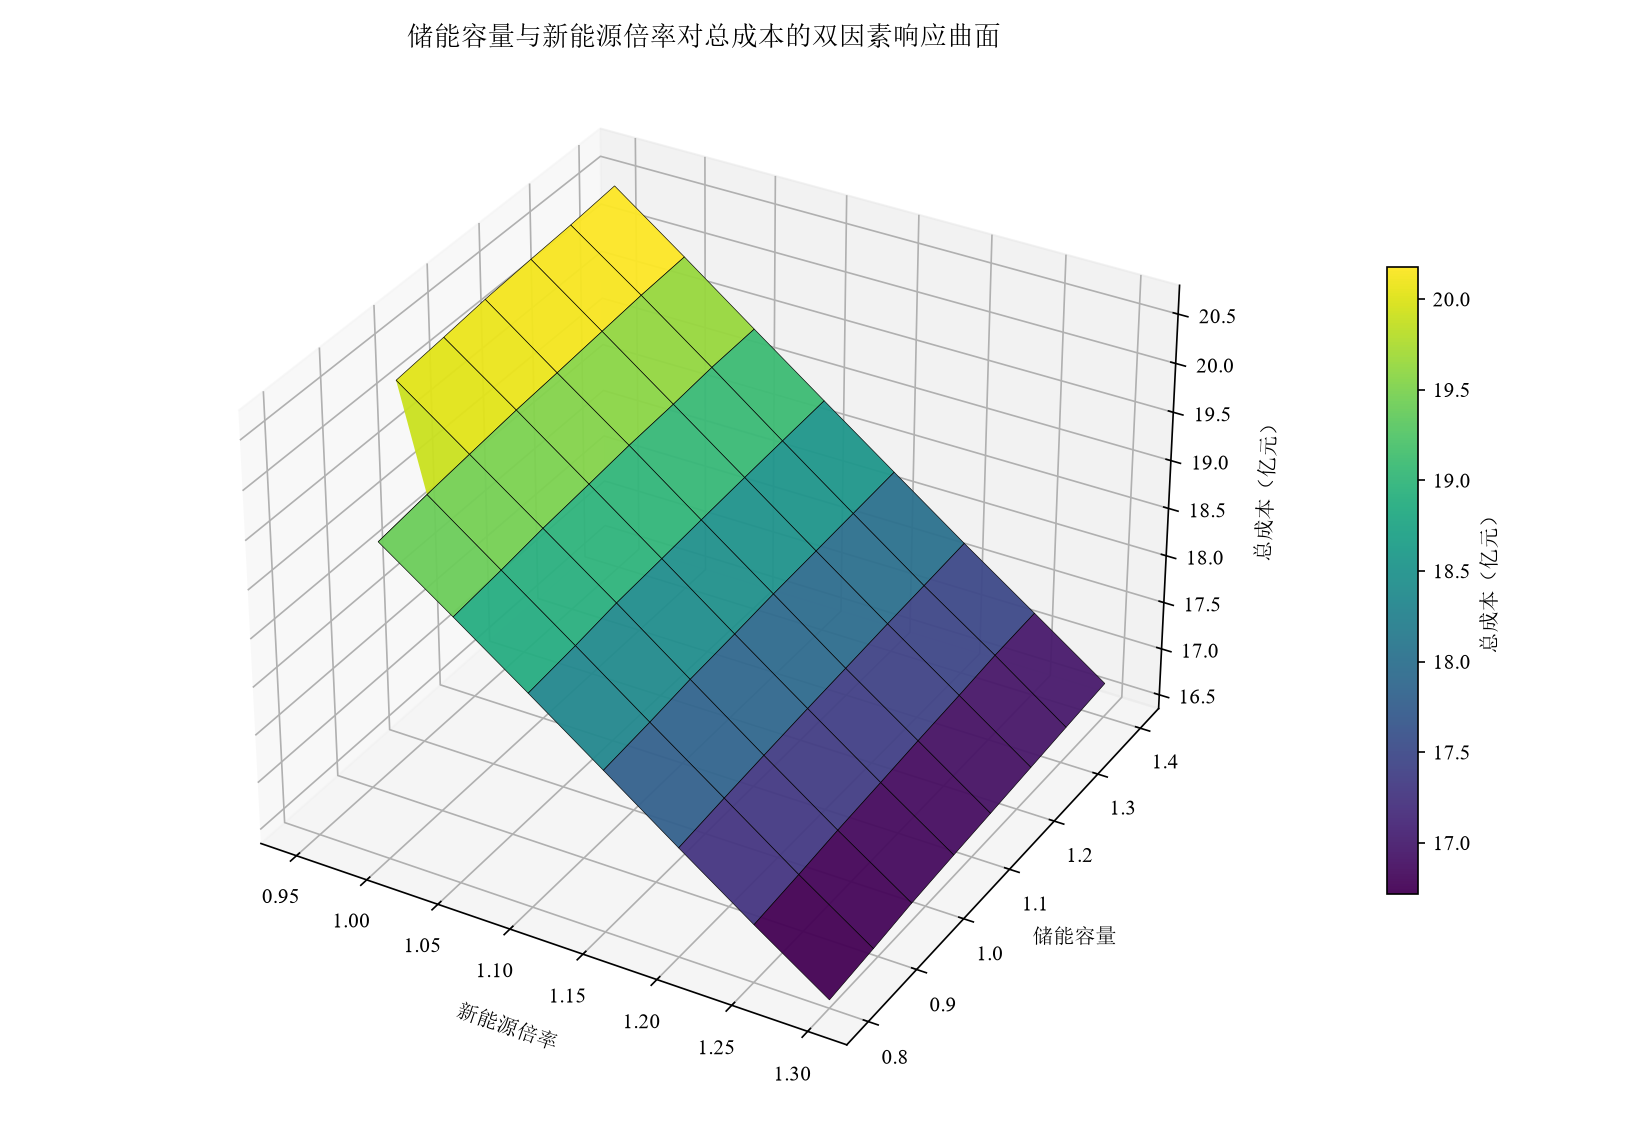
\includegraphics[width=1\textwidth]{figures/储能容量与新能源倍率对总成本的双因素响应曲面.png}
\caption{储能容量与新能源倍率对总成本的双因素响应曲面}
\end{figure}

图为储能容量（0.800~1.400倍）与新能源倍率（0.950~1.300倍）扫描下六区域储能LP总成本的三维响应曲面。曲面沿新能源倍率方向坡度陡峭：倍率由0.950增至1.300时，成本自约20.470亿元单调降至16.440亿元，降幅约19.700\%，说明新能源出力是成本的第一主导因素；沿储能容量方向则十分平缓，容量由0.800倍增至1.400倍仅使成本上升约0.200~0.300亿元（约1.500\%），源于充放电循环增加带来的损耗。两方向影响近乎独立、曲面近似倾斜平面，交互作用微弱；左前角低倍率、低容量区域为空白（不可行），对应新能源不足时净购电峰值越过购电上限的可行性边界。

\section{敏感性分析}

为量化关键参数对系统运行的影响，以问题四“碳感知联合调度+储能”方案为基准，对储能容量、储能功率、充放电效率、购电上限、新能源倍率与碳价进行单因素扫描，并进一步分析“储能容量×新能源倍率”的双因素交互及储能目标权重的影响。

\begin{figure}[H]
\centering
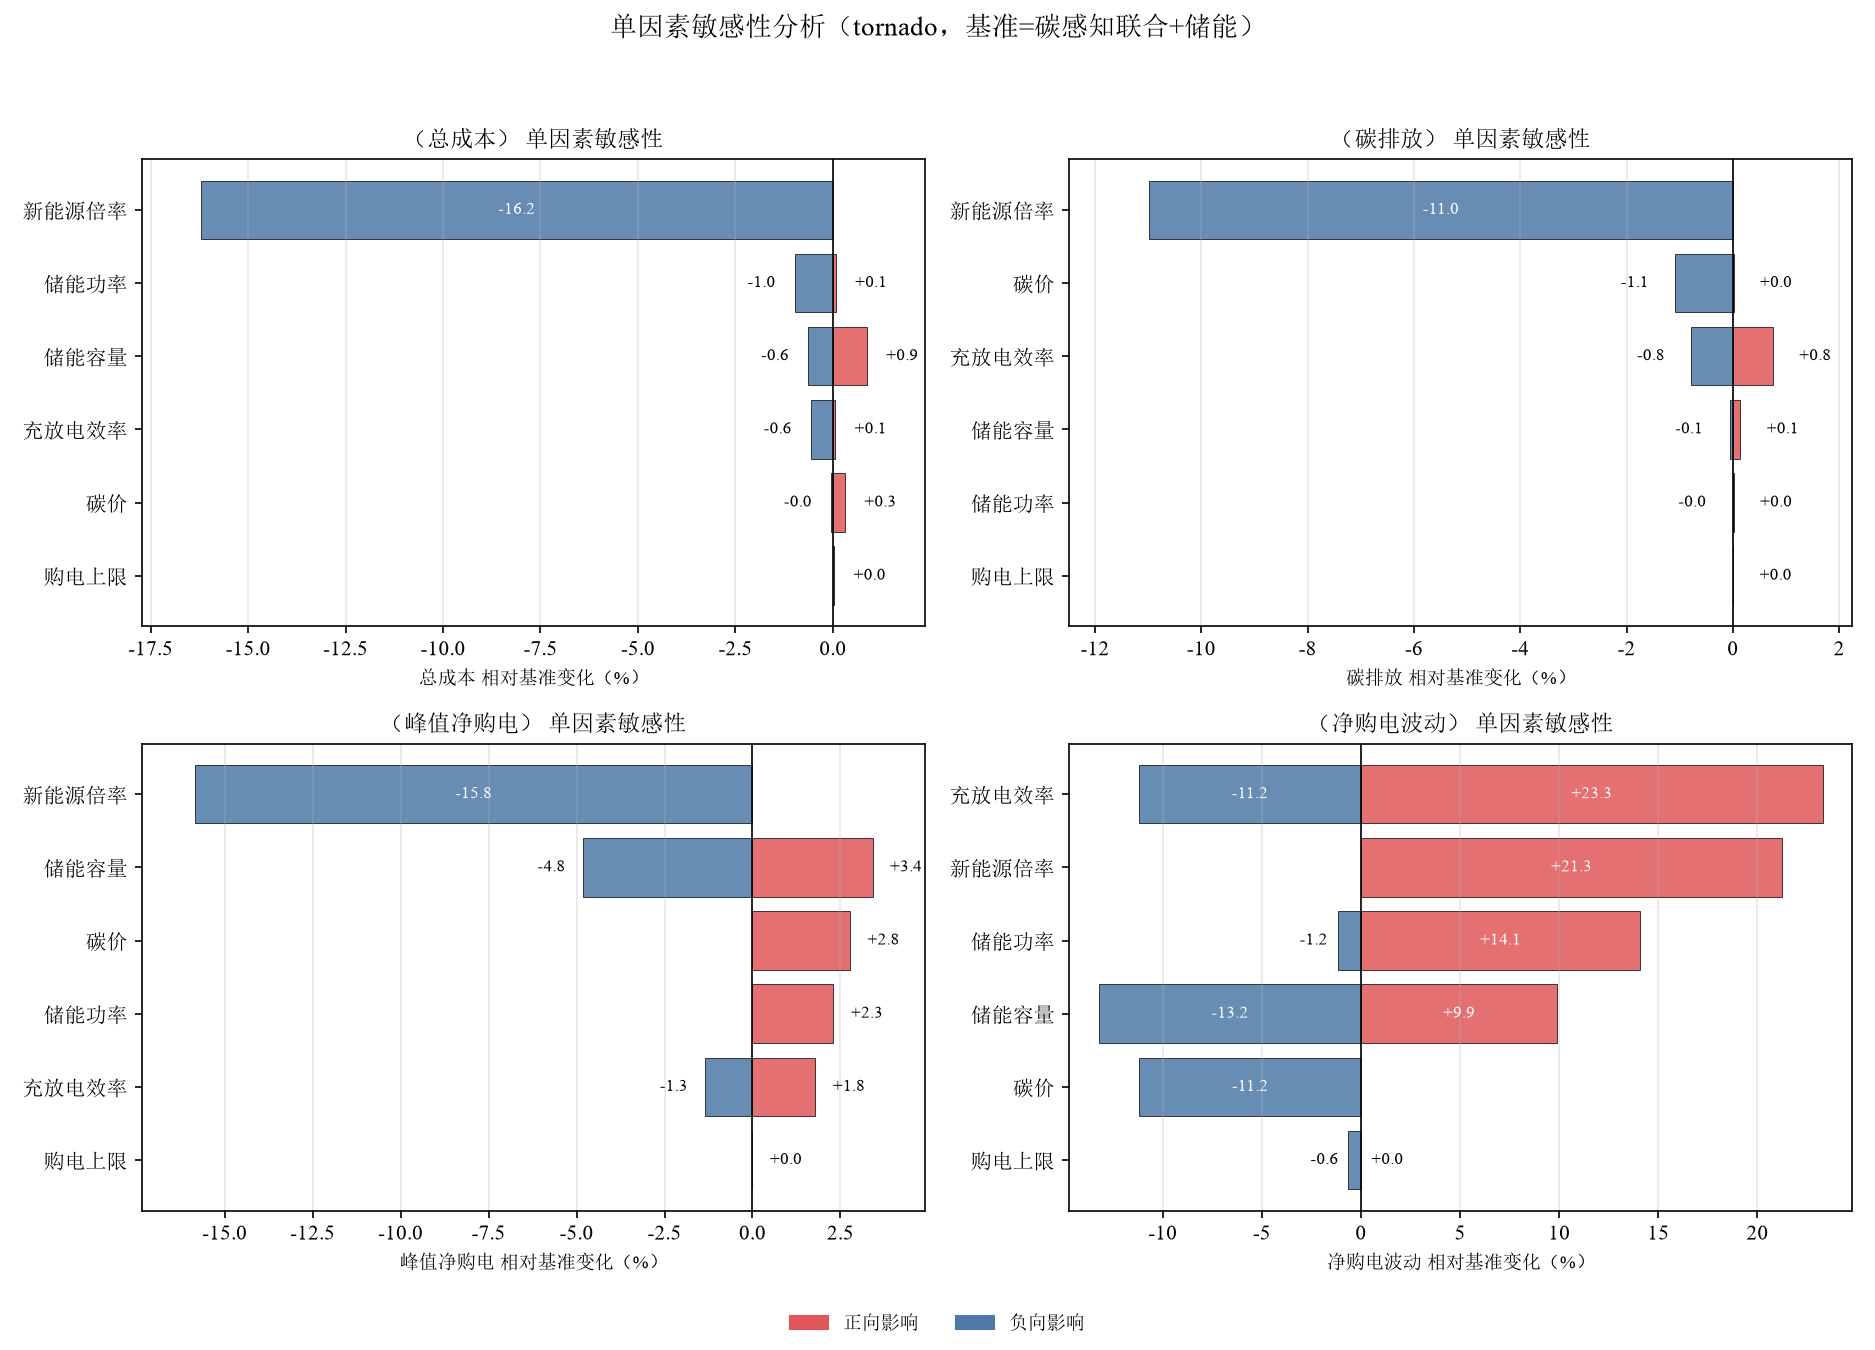
\includegraphics[width=1\textwidth]{figures/单因素敏感性分析.png}
\caption{单因素敏感性分析}
\end{figure}

新能源倍率是最强杠杆：提高15\%、30\%分别使成本下降8.200\%、16.200\%，碳排同步下降约5.500\%、11.000\%，峰值下降约8.000\%、15.800\%；但降至0.850倍及以下时，储能LP因无储能净购电峰值超出购电上限而不可行，购电边界成为低新能源场景的关键瓶颈。储能容量主要影响削峰平滑：容量由0.800倍增至1.400倍时，峰值由1952.000MW降至1796.800MW、波动由18.385万降至14.517万，但成本因充放电损耗与更多循环由19.632亿元升至19.928亿元；容量低于0.600倍亦不可行。充放电效率提高10\%可使成本、碳排与峰值分别下降约0.600\%、0.800\%、1.300\%，对波动的改善尤为显著（波动下降约11.200\%）。购电上限在基准取值下并不约束经济调度，但降低即触发不可行，说明其本质是系统可行性边界。碳价由0元/吨升至800元/吨时，碳排由211.601万吨降至209.486万吨，成本基本持平，表明在当前成本主导的调度与储能协同下，碳价的边际减排作用有限。

\section{模型检验}

本文在解决问题一时，依据统计分析结果进一步构建常数强度标记点过程预测模型和任务数+ GPU Mark +收缩融合预测模型，并比较两者的平均验证集得出后者预测效果，更优。为进一步检验模型适配性，本文以均值预测RMSE/$\sigma$=1为基准，引入基础的季节朴素模型、季节基准模型，计算结果得出RMSE/$\sigma$均大于1，后引入ETS/SES模型，平均验证集仍大于1。只有任务数+ GPU Mark +收缩融合预测模型结果优于均值预测，证明了所选模型适配度较高，也呼应了前文统计分析结论提到的“预测模型不宜过度依赖简单的季节周期结构”。

\begin{table}[H]\zihao{-5}
\centering
\caption{模型检验结果}
\begin{tabularx}{\textwidth}{>{\centering\arraybackslash}Xcc}
\toprule
模型& RMSE/$\sigma$ & 效果\\
\midrule
季节朴素模型 & 1.472 & 较差\\
季节基准模型 & 1.027 & ——\\
ETS/SES & 1.011 & ——\\
常数强度标记点过程 & 1.019 & ——\\
任务数+GPU·mark+收缩融合 & $0.949<1$ & 优于均值预测\\
\bottomrule
\end{tabularx}
\end{table}

表以均值预测RMSE/$\sigma$=1为基准对比五种模型。季节朴素（1.472）显著劣于均值，其余季节类模型与ETS/SES的比值均略大于1，仅任务数+GPU·mark+收缩融合模型达0.949，优于均值预测，验证其对任务到达随机结构的捕获能力，也说明预测不宜过度依赖简单季节周期结构。

\section{模型推广}
该求解框架具备较强泛化能力，可拓展至多数据中心集群、多云协同节点以及园区级源网荷储综合系统\cite{ding2022b}。仅需替换任务类型定义、各区域算力容量、功率映射关系、分时电价、碳强度系数、储能设备等核心参数，本模型便能够适配云计算任务编排、绿色算力跨域调度、园区用电需求响应、高比例新能源微电网负荷管控等现实业务场景。在此基础上接入时序滚动预测模块，可进一步升级构建模型预测控制架构，也可向鲁棒优化、随机优化方向拓展，处理实际场景中的各类不确定性。

\subsection{模型优点}

（1）构建了统一的功率映射、PUE折算、购售电交易以及新能源消纳核算口径，保障不同子问题之间评价标准一致，各算例输出结果具备横向可比性，便于开展多方案对比分析。

（2）搭建“ETS预测—碳感知调度—逐区域LP—净购电反馈”四层递进式求解框架，整体逻辑层次清晰；将任务离散组合决策与储能连续时序优化进行解耦处理，有效降低混合优化问题求解规模，控制模型计算复杂度，提升仿真运算效率。

（3）采用$\varepsilon$-constraint多目标求解、情景仿真、参数权重敏感性分析多重手段，把成本‑碳排放之间的权衡关系显性化，Pareto折中结果物理含义明确，模型输出可解释性强，方便决策者开展方案研判。

（4）引入净购电反馈环节，在调度逻辑层面打通算力任务与储能系统，形成算‑储协同闭环机制，能够定量评估储能参与调度带来的电网削峰、负荷平滑效果，量化算储协同模式的实际效益增益。

\subsection{模型缺点}

（1）任务分配环节采用贪心启发式策略，求解得到可行高质量解，受启发规则限制，无法严格保证整数规划意义下的全局最优，部分算例存在解的次优风险。

（2）预测模块依赖历史聚合算力样本，对于突发性、稀疏尖峰任务拟合捕获能力有限，面对AI训练类任务极端到达工况时预测偏差会显著增大，会向下游调度传递预测误差。

（3）模型全部场景参数采用确定性定值输入，没有引入随机变量显式刻画电价、新能源出力、任务到达等现实存在的概率不确定性，抗扰动能力有待进一步提升。

（4）对网络、电力系统做了适度简化，忽略迁移带宽约束、任务迁移能耗、跨区域电网潮流约束等现实要素，若要落地工程实际部署，还需要叠加更为精细的通信网络模型与电网运行约束。

\subsection*{AI工具使用声明}

本参赛队在竞赛过程中使用了AI工具，主要用于语言润色、代码调试等，详细使用情况见附录。

\newpage

\printbibliography

\newpage

\appendix
\section*{附录}
\subsection*{代码}

\begin{lstlisting}
import os, numpy as np, pandas as pd
from collections import defaultdict
import matplotlib; matplotlib.use('Agg')
import matplotlib.pyplot as plt
from matplotlib.patches import Patch

B=os.path.dirname(os.path.abspath(__file__)) if '__file__' in globals() else os.getcwd()
wt=pd.read_csv(f'{B}/workload_tasks.csv'); gpu=pd.read_csv(f'{B}/gpu_constraints.csv'); lat=pd.read_csv(f'{B}/network_latency.csv')
A=dict(zip(gpu.Region,gpu.Available_GPU)); RS=sorted(A)
L={(x.FromRegion,x.ToRegion):x.NetworkLatency_ms for x in lat.itertuples()}
ML={'RealTimeInference':20,'BatchInference':80,'AITraining':150}
T0=2376; TE=2406
fr=lambda s,t:[r for r in RS if L.get((s,r),1e9)<=ML[t]]
tk=wt[wt.ArrivalHour>=T0].sort_values(['ArrivalHour','TaskID']).copy()
tk['dh']=np.ceil(tk.EstimatedDuration_min/60).astype(int)
occ=defaultdict(int); S=[]
for t in tk.itertuples():
    tp=t.TaskType; src=t.SourceRegion; g=int(t.GPU_Demand); d=int(t.dh)
    f=fr(src,tp); o=[src]+sorted([r for r in f if r!=src],key=lambda r:-A[r])
    if tp=='RealTimeInference':
        s=int(t.ArrivalHour); rg=next((r for r in o if all(occ[r,h]+g<=A[r] for h in range(s,s+d))),max(f,key=lambda r:A[r]))
    else:
        rg=None
        for r in o:
            for s in range(int(t.ArrivalHour),min(int(t.LatestFinishHour),TE)-d+1):
                if all(occ[r,h]+g<=A[r] for h in range(s,s+d)): rg,s0=r,s; break
            if rg: break
        if rg is None: rg=max(f,key=lambda r:A[r]); s0=int(t.ArrivalHour)
        s=s0
    for h in range(s,s+d): occ[rg,h]+=g
    S.append((t.TaskID,tp,src,rg,s,s+d,g,d))
sc=pd.DataFrame(S,columns=['TaskID','TaskType','SourceRegion','Region','Start','End','GPU','Dur_h'])
sc.to_csv(f'{B}/schedule_2376_2406.csv',index=False,encoding='utf-8-sig')
print(f"Total={len(sc)}  cross2399={len(sc[sc.End>2399])}\ntype={sc.TaskType.value_counts().to_dict()}\nregion={sc.Region.value_counts().to_dict()}")
hrs=np.arange(T0,TE+1)
u=pd.DataFrame({r:[occ[r,h]/A[r]*100 for h in hrs] for r in RS},index=hrs)
print("Util% min~max:","  ".join(f"{r}:{u[r].min():.0f}~{u[r].max():.0f}" for r in RS))
print("Violations:",[bool((u[r]>100).any()) for r in RS])

plt.rcParams['font.family']='Times New Roman'
C={'RealTimeInference':'#e15759','BatchInference':'#4e79a7','AITraining':'#59a14f'}
LM={'RealTimeInference':'Real-Time Inference','BatchInference':'Batch Inference','AITraining':'AI Training'}

def lanes(d):
    d=d.sort_values(['Start','End','TaskID']).copy(); le=[]; li=[]
    for x in d.itertuples():
        k=next((i for i,e in enumerate(le) if e<=x.Start),None)
        if k is None: k=len(le); le.append(x.End)
        else: le[k]=x.End
        li.append(k)
    d['PlotLane']=li
    return d,max(len(le),1)

fig,ax=plt.subplots(figsize=(16,7.5)); ry={r:i for i,r in enumerate(RS)}; BH=0.68
for r in RS:
    d,n=lanes(sc[sc.Region==r])
    if not len(d): continue
    off=np.linspace(-BH/2,BH/2,n) if n>1 else np.zeros(1); lw=min(5.2,max(1.35,24./n))
    for x in d.itertuples(): ax.hlines(ry[r]+off[int(x.PlotLane)],x.Start,x.End,color=C[x.TaskType],linewidth=lw,alpha=.88,zorder=3)
ax.set_xlim(T0,TE); ax.set_xticks(np.arange(T0,TE+1,2))
ax.set_xlabel('Hour',fontsize=12); ax.set_ylabel('Execution Region',fontsize=12)
ax.set_yticks(list(ry.values())); ax.set_yticklabels(RS,fontsize=11)
ax.invert_yaxis(); ax.grid(axis='x',alpha=.24,linewidth=.8)
for y in np.arange(.5,len(RS)-.5,1): ax.axhline(y,color='0.86',linewidth=.8)
ax.axvline(2400,color='0.35',linestyle='--',linewidth=1.2,alpha=.85)
ax.text(2400.15,-.55,'Closure',fontsize=9.5,va='center',ha='left',color='0.30')
fig.legend(handles=[Patch(facecolor=C[t],edgecolor='none',label=LM[t]) for t in C],loc='upper center',bbox_to_anchor=(.5,.91),ncol=3,frameon=False)
fig.suptitle('Q1 Base Scheduling Gantt (2376-2406)',fontsize=14,y=.985)
fig.tight_layout(rect=[0,0,1,.865]); fig.savefig(f'{B}/gantt_real.png',dpi=300,bbox_inches='tight'); plt.close(fig)

fig,axes=plt.subplots(2,1,figsize=(13,8))
for r in RS: axes[0].plot(hrs,u[r],label=r)
axes[0].set_ylabel('GPU Utilization (%)'); axes[0].legend(ncol=3); axes[0].grid(alpha=.3); axes[0].set_title('Regional GPU Utilization (Last 24 h + Closure)')
sh=pd.DataFrame({r:{t:0. for t in C} for r in RS}).T
for x in sc.itertuples():
    for h in range(int(x.Start),int(x.End)): sh.loc[x.Region,x.TaskType]+=x.GPU
sh=sh.div(sh.sum(axis=1).replace(0,np.nan),axis=0).fillna(0)*100
b=np.zeros(len(RS))
for t in C:
    axes[1].bar(RS,sh[t],bottom=b,label=LM[t],color=C[t]); b+=sh[t].values
axes[1].set_ylabel('Type Share (%)'); axes[1].legend(); axes[1].grid(alpha=.3,axis='y'); axes[1].set_title('Per-Region Task-Type GPU Share (Total over Window)')
fig.tight_layout(); fig.savefig(f'{B}/utilization_share.png',dpi=180,bbox_inches='tight'); plt.close(fig)

print("\n==== Completed ====")
print(f"Schedule: {B}/schedule_2376_2406.csv\nGantt: {B}/gantt_real.png\nUtil: {B}/utilization_share.png")
\end{lstlisting}

\begin{lstlisting}
import argparse, math, os, time, warnings, zipfile
from dataclasses import dataclass
from pathlib import Path
import numpy as np, pandas as pd
import matplotlib as mpl, matplotlib.pyplot as plt
from matplotlib.colors import LinearSegmentedColormap
from matplotlib.patches import PathPatch, Rectangle
from matplotlib.path import Path as MplPath
from mpl_toolkits.mplot3d import Axes3D

EPS=[5,15,25,40,60,80,150]
W=(0.55,0.35,0.10)
TOP_K,SCAN,USAMP=12,240,6
ME,SET,NO,T=2399,2405,2406,2407
LIMIT_BASE,DPI,PDF,GANTT,TOL,QUICK=True,400,True,50,1e-6,5000

DARK,ORG,GOLD,LIGHT="#D47822","#EA9832","#F4B842","#FAD072"
BG,TXT,MUT,GRID,WH="#FFFDF7","#333333","#777777","#D9D9D9","#FFFFFF"
REG=["RegionA","RegionB","RegionC","RegionD","RegionE","RegionF"]
TY=["RealTimeInference","BatchInference","AITraining"]
TCN={"RealTimeInference":"实时推理","BatchInference":"批量推理","AITraining":"AI训练"}
SH={r:r[-1] for r in REG}
RC={"RegionA":LIGHT,"RegionB":LIGHT,"RegionC":GOLD,"RegionD":ORG,"RegionE":DARK,"RegionF":ORG}
cm=LinearSegmentedColormap.from_list

FILES={"tasks":"workload_tasks.csv","exo":"region_exogenous_inputs.csv","gpu":"gpu_constraints.csv",
       "latency":"network_latency.csv","power":"task_power_mapping.csv","storage":"storage_parameters_model.csv",
       "baseline":"baseline_reference_only.csv"}
REQ={"workload_tasks.csv":["TaskID","TaskType","ArrivalHour","GPU_Demand","EstimatedDuration_min","SourceRegion","MaxLatency_ms","LatestFinishHour","EarliestStartHour"],
     "region_exogenous_inputs.csv":["Hour","Region","ElectricityPrice_CNY_per_MWh","SellPrice_CNY_per_MWh","CarbonIntensity_tCO2_per_MWh","AvailableRenewable_MW","NonAI_IT_Load_MW"],
     "gpu_constraints.csv":["Region","Available_GPU","Max_IT_Power_MW","PUE","Max_Facility_Power_MW"],
     "network_latency.csv":["FromRegion","ToRegion","NetworkLatency_ms"],
     "task_power_mapping.csv":["TaskType","GPU_Power_MW_per_EquivalentGPU"],
     "storage_parameters_model.csv":["Region","SellLimit_MW","MaxGridImport_MW"],
     "baseline_reference_only.csv":["Hour","Region","UsedRenewable_MW","Baseline_AI_IT_Load_MW","GridPurchase_MW","GridSell_MW","CarbonEmission_tCO2"]}

def style():
    mpl.rcParams.update({"figure.facecolor":BG,"axes.facecolor":BG,"savefig.facecolor":BG,
        "axes.edgecolor":"#666666","axes.labelcolor":TXT,"text.color":TXT,"xtick.color":TXT,"ytick.color":TXT,
        "axes.grid":False,"grid.color":GRID,"grid.alpha":0.45,"grid.linewidth":0.7,
        "axes.spines.top":False,"axes.spines.right":False,"font.family":"sans-serif",
        "font.sans-serif":["Microsoft YaHei","SimHei","Noto Sans CJK SC","Source Han Sans SC","PingFang SC","Arial Unicode MS","DejaVu Sans"],
        "font.size":10.5,"axes.titlesize":12,"axes.titleweight":"semibold","axes.labelsize":10.5,
        "legend.fontsize":9,"figure.titlesize":13,"mathtext.fontset":"stix","axes.unicode_minus":False})

def save(fig,d,stem):
    d.mkdir(parents=True,exist_ok=True)
    fig.savefig(d/f"{stem}.png",dpi=DPI,bbox_inches="tight")
    if PDF: fig.savefig(d/f"{stem}.pdf",bbox_inches="tight")
    plt.close(fig); print(f"[图像] {stem}.png")

def unzip(base):
    if list(base.rglob("workload_tasks.csv")): return
    zs=[z for z in base.glob("*.zip") if "清洗后数据" in z.name] or list(base.glob("*.zip"))
    if not zs: return
    tgt=base/"_extracted_data"; tgt.mkdir(exist_ok=True)
    print(f"[数据] 解压 {zs[0].name} -> {tgt}")
    with zipfile.ZipFile(zs[0]) as f: f.extractall(tgt)

def find(base,fn):
    for sub in ["data","清洗后数据","_extracted_data","."]:
        p=base/sub
        if p.exists() and (cs:=list(p.rglob(fn))): return cs[0]
    cs=list(base.rglob(fn))
    if not cs: raise FileNotFoundError(f"找不到 {fn}，请把清洗后数据.zip 与脚本放在同一目录")
    return cs[0]

@dataclass
class D:
    tasks:pd.DataFrame; exo:pd.DataFrame; gpu:pd.DataFrame; latency:pd.DataFrame
    power:pd.DataFrame; storage:pd.DataFrame; baseline:pd.DataFrame

def load(base,quick=False):
    unzip(base); p={k:find(base,v) for k,v in FILES.items()}
    print("[数据] 使用文件："+("".join(f"\n  {k:9s}: {v}" for k,v in p.items())))
    data=D(tasks=pd.read_csv(p["tasks"]),exo=pd.read_csv(p["exo"]),gpu=pd.read_csv(p["gpu"]),
           latency=pd.read_csv(p["latency"]),power=pd.read_csv(p["power"]),
           storage=pd.read_csv(p["storage"]),baseline=pd.read_csv(p["baseline"]))
    if quick and len(data.tasks)>QUICK:
        data.tasks=data.tasks.sort_values(["ArrivalHour","TaskID"]).iloc[:QUICK].copy()
        print(f"[快速模式] 仅处理前 {QUICK:,} 个任务")
    for k,v in [("tasks","workload_tasks.csv"),("exo","region_exogenous_inputs.csv"),("gpu","gpu_constraints.csv"),
                ("latency","network_latency.csv"),("power","task_power_mapping.csv"),("storage","storage_parameters_model.csv"),
                ("baseline","baseline_reference_only.csv")]:
        df=getattr(data,k); miss=[c for c in REQ[v] if c not in df.columns]
        if miss: raise ValueError(f"{v} 缺少字段: {miss}")
    bt=set(data.tasks.TaskType)-set(TY)
    if bt: warnings.warn(f"未识别TaskType: {bt}")
    print(f"[数据] 任务数：{len(data.tasks):,}；区域数：{data.exo.Region.nunique()}；时段：{data.exo.Hour.min()}~{data.exo.Hour.max()}")
    return data

@dataclass
class MA:
    price:np.ndarray; sell_price:np.ndarray; carbon:np.ndarray; renewable:np.ndarray; nonai:np.ndarray
    baseline_used:np.ndarray; baseline_ai:np.ndarray; gpu:np.ndarray; max_it:np.ndarray; pue:np.ndarray
    max_fac:np.ndarray; sell_lim:np.ndarray; max_import:np.ndarray; lat:np.ndarray
    pmap:dict; r2i:dict; i2r:dict; score:np.ndarray

def mm(x):
    lo,hi=np.nanmin(x),np.nanmax(x)
    return np.zeros_like(x,float) if hi<=lo+1e-12 else (x-lo)/(hi-lo)

def build(data):
    r2i={r:i for i,r in enumerate(REG)}; i2r={i:r for r,i in r2i.items()}
    R,T_=len(REG),T
    def mlong(df,val,fill=np.nan):
        pv=df.pivot_table(index="Region",columns="Hour",values=val,aggfunc="first").reindex(index=REG,columns=range(T_))
        a=pv.to_numpy(float)
        if np.isnan(a).any(): a=pv.ffill(axis=1).bfill(axis=1).fillna(fill).to_numpy(float)
        return a
    price=mlong(data.exo,"ElectricityPrice_CNY_per_MWh",0.); sell=mlong(data.exo,"SellPrice_CNY_per_MWh",0.)
    carbon=mlong(data.exo,"CarbonIntensity_tCO2_per_MWh",0.); re=mlong(data.exo,"AvailableRenewable_MW",0.)
    nonai=mlong(data.exo,"NonAI_IT_Load_MW",0.)
    bused=mlong(data.baseline,"UsedRenewable_MW",0.); bai=mlong(data.baseline,"Baseline_AI_IT_Load_MW",0.)
    gi=data.gpu.set_index("Region").reindex(REG)
    storage=data.storage.set_index("Region").reindex(REG)
    lat=np.full((R,R),np.inf)
    for x in data.latency.itertuples(index=False):
        if x.FromRegion in r2i and x.ToRegion in r2i: lat[r2i[x.FromRegion],r2i[x.ToRegion]]=float(x.NetworkLatency_ms)
    pmap=dict(zip(data.power.TaskType,data.power.GPU_Power_MW_per_EquivalentGPU.astype(float)))
    score=W[0]*mm(price)+W[1]*mm(carbon)-0.10*mm(re)
    return MA(price,sell,carbon,re,nonai,bused,bai,gi.Available_GPU.to_numpy(float),gi.Max_IT_Power_MW.to_numpy(float),
              gi.PUE.to_numpy(float),gi.Max_Facility_Power_MW.to_numpy(float),storage.SellLimit_MW.fillna(0).to_numpy(float),
              storage.MaxGridImport_MW.fillna(np.inf).to_numpy(float),lat,pmap,r2i,i2r,score)

def overlap(dur):
    h=float(dur)/60.; n=max(1,int(math.ceil(h-1e-12)))
    a=np.ones(n,float); a[-1]=min(max(h-(n-1),1e-9),1.0); return a

def latest_start(row,n):
    lf=min(int(row.LatestFinishHour),NO); dh=float(row.EstimatedDuration_min)/60.
    return min(int(math.floor(lf-dh+1e-9)),SET-n+1)

def score_tables(a):
    out={}
    for n in range(1,9):
        if n==1: tab=a.score.copy()
        else:
            cs=np.cumsum(np.pad(a.score,((0,0),(1,0))),axis=1)
            tab=np.full_like(a.score,np.inf); tab[:,:T-n+1]=(cs[:,n:]-cs[:,:-n])/n
        out[n]=tab
    return out

def orders(st):
    return {n:{r:np.argsort(tab[r]) for r in range(tab.shape[0])} for n,tab in st.items()}

def cand_starts(r,earliest,latest,n,ords,st):
    if latest<earliest: return []
    cand=[]
    for s in ords[n][r][:SCAN]:
        s=int(s)
        if earliest<=s<=latest:
            cand.append(s)
            if len(cand)>=TOP_K: break
    if len(cand)<max(4,TOP_K//2) and latest-earliest+1<=400:
        loc=st[n][r,earliest:latest+1]; k=min(TOP_K,len(loc))
        if k>0: cand.extend((earliest+np.argpartition(loc,k-1)[:k]).tolist())
    if latest>earliest:
        cand.extend(np.linspace(earliest,latest,min(USAMP,latest-earliest+1),dtype=int).tolist())
    cand=sorted(set(int(x) for x in cand+[earliest,latest] if earliest<=x<=latest))
    cand.sort(key=lambda s:st[n][r,s]); return cand[:max(TOP_K,6)]

def feas_regions(row,eps,a):
    src=a.r2i[row.SourceRegion]
    if row.TaskType=="RealTimeInference": return [src]
    cap=min(float(row.MaxLatency_ms),float(eps))
    return [r for r in range(len(REG)) if a.lat[src,r]<=cap+1e-9]

def schedule_eps(data,a,eps,st,ords,verbose=True):
    R,T_=len(REG),T
    occ=np.zeros((R,T_),np.float32); ai=np.zeros((R,T_),np.float32)
    cap=np.maximum(np.minimum(a.max_it[:,None]-a.nonai,a.max_fac[:,None]/a.pue[:,None]-a.nonai),0.)
    tasks=data.tasks.copy()
    dh=tasks.EstimatedDuration_min.to_numpy(float)/60.
    slack=np.minimum(tasks.LatestFinishHour.to_numpy(float),NO)-tasks.EarliestStartHour.to_numpy(float)-dh
    tasks["_p"]=np.where(tasks.TaskType.eq("RealTimeInference"),-1e9,slack)
    tasks=tasks.sort_values(["_p","ArrivalHour","TaskID"]).reset_index(drop=True)
    rows=[]; inf=[]; t0=time.time()
    def ok(r,s,e,gpu,power,prof):
        if e>T_ or e-1>SET: return None
        ga=gpu*prof
        if np.any(occ[r,s:e]+ga>a.gpu[r]+1e-7): return None
        aa=gpu*power*prof
        if np.any(ai[r,s:e]+aa>cap[r,s:e]+TOL): return None
        it=a.nonai[r,s:e]+ai[r,s:e]+aa; tot=it*a.pue[r]
        dr=np.minimum(tot,np.minimum(a.baseline_used[r,s:e],a.renewable[r,s:e])) if LIMIT_BASE else np.minimum(tot,a.renewable[r,s:e])
        if np.any(np.maximum(tot-dr,0.)>a.max_import[r]+TOL): return None
        return ga,aa
    for k,row in enumerate(tasks.itertuples(index=False)):
        tp=row.TaskType; src=a.r2i[row.SourceRegion]; gpu=float(row.GPU_Demand)
        pp=float(a.pmap[tp]); prof=overlap(row.EstimatedDuration_min); n=len(prof)
        earliest=max(int(row.ArrivalHour),int(row.EarliestStartHour),0); latest=latest_start(row,n)
        if tp=="RealTimeInference": earliest=latest=int(row.ArrivalHour)
        if latest<earliest: inf.append(row.TaskID); continue
        regs=feas_regions(row,eps,a)
        if not regs: inf.append(row.TaskID); continue
        best=None; bs=np.inf
        for r in regs:
            starts=[earliest] if tp=="RealTimeInference" else cand_starts(r,earliest,latest,n,ords,st)
            for s in starts:
                e=s+n; hit=ok(r,s,e,gpu,pp,prof)
                if hit is None: continue
                lat=a.lat[src,r]
                es=float(np.average(a.score[r,s:e],weights=prof))
                sc=es+W[2]*lat/max(150.,float(row.MaxLatency_ms),1.)+0.00015*max(0,s-int(row.ArrivalHour))
                if sc<bs: bs=sc; best=(r,s,e,lat)+hit
        if best is None and tp!="RealTimeInference":
            for r in regs:
                f=0
                for s in range(earliest,latest+1):
                    e=s+n; hit=ok(r,s,e,gpu,pp,prof)
                    if hit is None: continue
                    lat=a.lat[src,r]
                    sc=float(np.average(a.score[r,s:e],weights=prof))+W[2]*lat/max(150.,float(row.MaxLatency_ms),1.)+0.00015*max(0,s-int(row.ArrivalHour))
                    if sc<bs: bs=sc; best=(r,s,e,lat)+hit
                    f+=1
                    if f>=3: break
        if best is None: inf.append(row.TaskID); continue
        r,s,e,lat,ga,aa=best
        occ[r,s:e]+=ga; ai[r,s:e]+=aa
        rows.append({"TaskID":row.TaskID,"TaskType":tp,"ArrivalHour":int(row.ArrivalHour),"SourceRegion":row.SourceRegion,
            "ExecuteRegion":a.i2r[r],"StartHour":int(s),"FinishHour":float(s+row.EstimatedDuration_min/60.),
            "Duration_h":float(row.EstimatedDuration_min/60.),"GPU_Demand":gpu,"NetworkLatency_ms":lat,
            "MaxLatency_ms":float(row.MaxLatency_ms),"IsMigrated":int(a.i2r[r]!=row.SourceRegion),
            "Delay_h":float(s-int(row.ArrivalHour)),"AI_IT_Energy_MWh":float(gpu*pp*row.EstimatedDuration_min/60.),
            "GreedyScore":float(bs),"epsilon_latency_ms":float(eps)})
        if verbose and (k+1)%5000==0:
            print(f"  eps={eps:>5}: {k+1:>6}/{len(tasks)} ({100*(k+1)/len(tasks):5.1f}%)，不可行 {len(inf):,}，耗时 {time.time()-t0:.1f}s")
    return pd.DataFrame(rows),ai.astype(float),occ.astype(float),inf

def settle(ai,a):
    R,T_=ai.shape
    it=a.nonai+ai; tot=it*a.pue[:,None]
    dr=np.minimum(tot,a.baseline_used) if LIMIT_BASE else np.minimum(tot,a.renewable)
    dr=np.minimum(dr,a.renewable)
    sell=np.minimum(np.maximum(a.renewable-dr,0.),a.sell_lim[:,None])
    gbuy=np.maximum(tot-dr,0.); curt=np.maximum(a.renewable-dr-sell,0.); net=gbuy-sell
    cost=gbuy*a.price-sell*a.sell_price; carb=gbuy*a.carbon
    viol=np.maximum(gbuy-a.max_import[:,None],0.)
    rows=[]
    for r in range(R):
        for h in range(T_):
            rows.append({"Hour":h,"Region":REG[r],"Optimized_AI_IT_Load_MW":ai[r,h],"NonAI_IT_Load_MW":a.nonai[r,h],
                "IT_Load_MW":it[r,h],"Total_Load_MW":tot[r,h],"ElectricityPrice_CNY_per_MWh":a.price[r,h],
                "SellPrice_CNY_per_MWh":a.sell_price[r,h],"CarbonIntensity_tCO2_per_MWh":a.carbon[r,h],
                "AvailableRenewable_MW":a.renewable[r,h],"DirectRenewable_MW":dr[r,h],"GridPurchase_MW":gbuy[r,h],
                "GridSell_MW":sell[r,h],"Curtailment_MW":curt[r,h],"NetGridImport_MW":net[r,h],
                "ElectricityCost_CNY":cost[r,h],"CarbonEmission_tCO2":carb[r,h],"GridImportViolation_MW":viol[r,h]})
    return pd.DataFrame(rows)

def add_base(hourly,data):
    b=data.baseline[["Hour","Region","Baseline_AI_IT_Load_MW","UsedRenewable_MW","GridPurchase_MW","GridSell_MW","NetGridImport_MW","CarbonEmission_tCO2"]].copy()
    b=b.rename(columns={"UsedRenewable_MW":"Baseline_UsedRenewable_MW","GridPurchase_MW":"Baseline_GridPurchase_MW",
        "GridSell_MW":"Baseline_GridSell_MW","NetGridImport_MW":"Baseline_NetGridImport_MW","CarbonEmission_tCO2":"Baseline_CarbonEmission_tCO2"})
    return hourly.merge(b,on=["Hour","Region"],how="left")

def metrics(sd,h,a,eps):
    if sd.empty:
        totlat,avlat,mig,rate,gpuh=np.nan,np.nan,0,np.nan,0.
    else:
        totlat=sd.NetworkLatency_ms.sum(); avlat=sd.NetworkLatency_ms.mean()
        mig=int(sd.IsMigrated.sum()); rate=100*mig/len(sd)
        gpuh=float((sd.loc[sd.IsMigrated.eq(1),"GPU_Demand"]*sd.loc[sd.IsMigrated.eq(1),"Duration_h"]).sum())
    are=h.AvailableRenewable_MW.sum(); util=100*(h.DirectRenewable_MW.sum()+h.GridSell_MW.sum())/are if are>0 else np.nan
    return {"epsilon_latency_ms":float(eps),"TotalCost_CNY":float(h.ElectricityCost_CNY.sum()),
        "TotalCarbon_tCO2":float(h.CarbonEmission_tCO2.sum()),"TotalLatency_ms":float(totlat),
        "AverageLatency_ms":float(avlat),"RenewableUtilization_pct":float(util),
        "PeakNetGridImport_MW":float(h.groupby("Region").NetGridImport_MW.max().sum()),
        "MigrationCount":mig,"MigrationRate_pct":float(rate),"MigrationGPUHours":gpuh,
        "ScheduledTaskCount":int(len(sd)),"GridImportViolation_MWh":float(h.GridImportViolation_MW.sum())}

def pareto_nd(df):
    if df.empty: return df.copy()
    p=df.sort_values("epsilon_latency_ms").copy()
    key=pd.DataFrame({"ck":p.TotalCost_CNY.round(4),"bk":p.TotalCarbon_tCO2.round(4),
        "lk":p.AverageLatency_ms.round(6),"rk":p.RenewableUtilization_pct.round(6)},index=p.index)
    p=p.loc[~key.duplicated(keep="first")].copy()
    vals=np.column_stack([p.TotalCost_CNY.to_numpy(float),p.TotalCarbon_tCO2.to_numpy(float),
        p.AverageLatency_ms.to_numpy(float),-p.RenewableUtilization_pct.to_numpy(float)])
    keep=np.ones(len(p),bool)
    for i in range(len(p)):
        for j in range(len(p)):
            if i!=j and np.all(vals[j]<=vals[i]+1e-12) and np.any(vals[j]<vals[i]-1e-12):
                keep[i]=False; break
    out=p.iloc[np.where(keep)[0]].copy(); out["IsPareto"]=1
    return out.sort_values("epsilon_latency_ms").reset_index(drop=True)

def rec_sol(p):
    if p.empty: return None
    q=p.copy(); score=np.zeros(len(q))
    for c in ["TotalCost_CNY","TotalCarbon_tCO2","AverageLatency_ms"]:
        x=q[c].to_numpy(float); den=np.nanmax(x)-np.nanmin(x)
        z=np.zeros_like(x) if den<=1e-12 else (x-np.nanmin(x))/den; score+=z**2
    x=q["RenewableUtilization_pct"].to_numpy(float); den=np.nanmax(x)-np.nanmin(x)
    z=np.zeros_like(x) if den<=1e-12 else (np.nanmax(x)-x)/den; score+=z**2
    return q.iloc[int(np.nanargmin(np.sqrt(score)))]

def constraint_check(sd,h,occ,a):
    tol=TOL; rows=[]
    def piv(v):
        return h.pivot_table(index="Region",columns="Hour",values=v,aggfunc="first").reindex(index=REG,columns=range(T)).to_numpy(float)
    ge=np.maximum(occ-a.gpu[:,None],0.); rows.append(["GPU capacity",float(ge.max()),"Equivalent GPU",bool(ge.max()<=tol)])
    for name,mat,lim,unit in [("IT power",piv("IT_Load_MW"),a.max_it,"MW"),("Facility power",piv("Total_Load_MW"),a.max_fac,"MW"),("Max grid import",piv("GridPurchase_MW"),a.max_import,"MW")]:
        ex=np.maximum(mat-lim[:,None],0.); rows.append([name,float(np.nanmax(ex)),unit,bool(np.nanmax(ex)<=tol)])
    if sd.empty: mlv,mfv,rsv=np.nan,np.nan,np.nan
    else:
        mlv=np.maximum(sd.NetworkLatency_ms.to_numpy(float)-sd.MaxLatency_ms.to_numpy(float),0.).max()
        mfv=np.maximum(sd.FinishHour.to_numpy(float)-NO,0.).max()
        rt=sd[sd.TaskType.eq("RealTimeInference")]
        rsv=0. if rt.empty else np.abs(rt.StartHour.to_numpy(float)-rt.ArrivalHour.to_numpy(float)).max()
    rows.extend([["Task network latency",float(mlv),"ms",bool(mlv<=tol)],["Finish before hour 2406",float(mfv),"h",bool(mfv<=tol)],
        ["Realtime start at arrival",float(rsv),"h",bool(rsv<=tol)]])
    return pd.DataFrame(rows,columns=["Constraint","MaxViolation","Unit","Passed"])

def mig_matrix(sd):
    if sd.empty: return pd.DataFrame(columns=["SourceRegion","ExecuteRegion","TaskType","TaskCount","GPUHours"])
    x=sd.copy(); x["GPUHours"]=x.GPU_Demand*x.Duration_h
    return x.groupby(["SourceRegion","ExecuteRegion","TaskType"],as_index=False).agg(TaskCount=("TaskID","count"),GPUHours=("GPUHours","sum"))

def region_summary(h,a):
    rows=[]
    for r in range(len(REG)):
        x=h[h.Region.eq(REG[r])]; tre=x.AvailableRenewable_MW.sum()
        ou=100*(x.DirectRenewable_MW.sum()+x.GridSell_MW.sum())/tre if tre>0 else np.nan
        bu=100*(x.Baseline_UsedRenewable_MW.sum()+x.Baseline_GridSell_MW.sum())/tre if tre>0 else np.nan
        rows.append({"Region":REG[r],"AvgElectricityPrice":a.price[r].mean(),"AvgCarbonIntensity":a.carbon[r].mean(),
            "AvailableGPU":a.gpu[r],"TotalAvailableRenewable_MWh":tre,"BaselineAIEnergy_MWh":x.Baseline_AI_IT_Load_MW.sum(),
            "OptimizedAIEnergy_MWh":x.Optimized_AI_IT_Load_MW.sum(),"BaselineGridPurchase_MWh":x.Baseline_GridPurchase_MW.sum(),
            "OptimizedGridPurchase_MWh":x.GridPurchase_MW.sum(),"BaselineCarbon_tCO2":x.Baseline_CarbonEmission_tCO2.sum(),
            "OptimizedCarbon_tCO2":x.CarbonEmission_tCO2.sum(),"BaselineRenewableUtil_pct":bu,"OptimizedRenewableUtil_pct":ou})
    return pd.DataFrame(rows)

def q2_summary(h,sd):
    bc=(h.Baseline_GridPurchase_MW*h.ElectricityPrice_CNY_per_MWh-h.Baseline_GridSell_MW*h.SellPrice_CNY_per_MWh).sum()
    oc=h.ElectricityCost_CNY.sum(); tre=h.AvailableRenewable_MW.sum()
    bru=100*(h.Baseline_UsedRenewable_MW.sum()+h.Baseline_GridSell_MW.sum())/tre
    oru=100*(h.DirectRenewable_MW.sum()+h.GridSell_MW.sum())/tre
    out=pd.DataFrame([["Total Cost (CNY)",bc,oc],["Carbon Emission (tCO2)",h.Baseline_CarbonEmission_tCO2.sum(),h.CarbonEmission_tCO2.sum()],
        ["Renewable Utilization (%)",bru,oru],["Peak Net Grid Import (MW)",h.groupby("Region").Baseline_NetGridImport_MW.max().sum(),h.groupby("Region").NetGridImport_MW.max().sum()]],
        columns=["Metric","Baseline","Optimized"])
    out["Change_pct"]=np.where(np.abs(out.Baseline)>1e-12,100*(out.Optimized-out.Baseline)/out.Baseline,np.nan)
    extra=pd.DataFrame([["Average Network Latency (ms)",np.nan,sd.NetworkLatency_ms.mean()],["Migrated Tasks",0.,sd.IsMigrated.sum()],
        ["Migration Rate (%)",0.,100*sd.IsMigrated.mean()]],columns=["Metric","Baseline","Optimized"]); extra["Change_pct"]=np.nan
    return pd.concat([out,extra],ignore_index=True)

def plot1(rs,fig_dir):
    df=rs.copy(); x=df.AvgElectricityPrice; y=df.AvgCarbonIntensity
    gpu=df.AvailableGPU.to_numpy(float); re=df.TotalAvailableRenewable_MWh.to_numpy(float)
    size=260+900*(gpu-gpu.min())/max(gpu.max()-gpu.min(),1)
    re_n=(re-re.min())/max(re.max()-re.min(),1)
    cmap=cm("orange_gold",[LIGHT,GOLD,DARK])
    fig,ax=plt.subplots(figsize=(7.2,5.4))
    sc=ax.scatter(x,y,s=size,c=re_n,cmap=cmap,edgecolor=DARK,linewidth=1.2,alpha=0.88)
    for _,r in df.iterrows(): ax.annotate(r.Region,(r.AvgElectricityPrice,r.AvgCarbonIntensity),xytext=(6,6),textcoords="offset points",fontsize=9.5,weight="semibold")
    ax.set_xlabel("平均电价 (CNY/MWh)"); ax.set_ylabel("平均碳强度 (tCO$_2$/MWh)")
    ax.set_title("六区域算力—能源特征分布"); ax.grid(True,linestyle="--",alpha=0.35)
    cbar=fig.colorbar(sc,ax=ax,pad=0.02); cbar.set_label("新能源资源强度（归一化）")
    ax.text(0.01,-0.18,"注：气泡大小表示可调度GPU容量；颜色深浅表示累计可用新能源水平。",transform=ax.transAxes,fontsize=8.5,color=MUT)
    save(fig,fig_dir,"Fig_Q2_01_region_characteristics")

def _rib(ax,x0,x1,y0a,y0b,y1a,y1b,color,alpha=0.45):
    verts=[(x0,y0a),(x0+0.35*(x1-x0),y0a),(x1-0.35*(x1-x0),y1a),(x1,y1a),(x1,y1b),
           (x1-0.35*(x1-x0),y1b),(x0+0.35*(x1-x0),y0b),(x0,y0b),(x0,y0a)]
    codes=[MplPath.MOVETO,MplPath.CURVE4,MplPath.CURVE4,MplPath.CURVE4,MplPath.LINETO,
           MplPath.CURVE4,MplPath.CURVE4,MplPath.CURVE4,MplPath.CLOSEPOLY]
    ax.add_patch(PathPatch(MplPath(verts,codes),facecolor=color,edgecolor="none",alpha=alpha))

def plot2(sd,fig_dir):
    da=sd.copy()
    if da.empty: return
    rate=100*da.IsMigrated.mean(); df=da[da.IsMigrated.eq(1)].copy()
    if df.empty: return
    df["GPUHours"]=df.GPU_Demand*df.Duration_h
    sn=[r for r in REG if r in set(df.SourceRegion)]; tn=[t for t in ["AITraining","BatchInference"] if t in set(df.TaskType)]
    dn=[r for r in REG if r in set(df.ExecuteRegion)]
    g1=df.groupby(["SourceRegion","TaskType"]).GPUHours.sum(); g2=df.groupby(["TaskType","ExecuteRegion"]).GPUHours.sum()
    xc=[0.10,0.50,0.90]; gap=0.025
    def pos(nodes,tots):
        tv=max(sum(tots.values()),1e-9); scale=(0.84-gap*(len(nodes)-1))/tv; pos={}; y=0.08
        for n in nodes:
            h=max(tots.get(n,0.)*scale,0.006); pos[n]=[y,y+h]; y+=h+gap
        return pos,scale
    spos,sc_=pos(sn,df.groupby("SourceRegion").GPUHours.sum().to_dict())
    tpos,_=pos(tn,df.groupby("TaskType").GPUHours.sum().to_dict())
    dpos,_=pos(dn,df.groupby("ExecuteRegion").GPUHours.sum().to_dict())
    tcol={"AITraining":DARK,"BatchInference":GOLD}
    fig,ax=plt.subplots(figsize=(10.2,6.8))
    sc_cur={k:v[0] for k,v in spos.items()}; tc_in={k:v[0] for k,v in tpos.items()}
    for s in sn:
        for tt in tn:
            v=float(g1.get((s,tt),0.))
            if v<=0: continue
            h=v*sc_; _rib(ax,xc[0]+0.015,xc[1]-0.020,sc_cur[s],sc_cur[s]+h,tc_in[tt],tc_in[tt]+h,tcol[tt],0.35)
            sc_cur[s]+=h; tc_in[tt]+=h
    tc_out={k:v[0] for k,v in tpos.items()}; dc={k:v[0] for k,v in dpos.items()}
    for tt in tn:
        for d in dn:
            v=float(g2.get((tt,d),0.))
            if v<=0: continue
            h=v*sc_; _rib(ax,xc[1]+0.020,xc[2]-0.015,tc_out[tt],tc_out[tt]+h,dc[d],dc[d]+h,tcol[tt],0.40)
            tc_out[tt]+=h; dc[d]+=h
    nw=0.025
    for n in sn:
        y0,y1=spos[n]; ax.add_patch(Rectangle((xc[0]-nw/2,y0),nw,y1-y0,facecolor=RC[n],edgecolor=WH,linewidth=0.8))
        ax.text(xc[0]-0.025,(y0+y1)/2,n,ha="right",va="center",fontsize=9.2,weight="semibold")
    for n in tn:
        y0,y1=tpos[n]; ax.add_patch(Rectangle((xc[1]-nw/2,y0),nw,y1-y0,facecolor=tcol[n],edgecolor=WH,linewidth=0.8))
        ax.text(xc[1],(y0+y1)/2,TCN[n],ha="center",va="center",fontsize=10.,weight="semibold",color=TXT)
    for n in dn:
        y0,y1=dpos[n]; ax.add_patch(Rectangle((xc[2]-nw/2,y0),nw,y1-y0,facecolor=RC[n],edgecolor=WH,linewidth=0.8))
        ax.text(xc[2]+0.025,(y0+y1)/2,n,ha="left",va="center",fontsize=9.2,weight="semibold")
    for x,lab in zip(xc,["任务来源区域","迁移任务类型","优化执行区域"]): ax.text(x,0.965,lab,ha="center",va="bottom",fontsize=11,weight="semibold")
    ax.set_title(f"跨区域弹性任务迁移流向（迁移 {int(da.IsMigrated.sum()):,} 个任务，迁移率 {rate:.1f}%）",pad=14)
    ax.set_xlim(0,1); ax.set_ylim(0.02,1); ax.axis("off")
    ax.text(0.5,0.025,"注：仅展示实际发生跨区域迁移的任务；流带宽度按 GPU-hours 加权，实时推理任务固定本区执行。",ha="center",va="bottom",fontsize=8.6,color=MUT)
    save(fig,fig_dir,"Fig_Q2_02_migration_sankey")

def plot3(h,fig_dir):
    def piv(v): return h.pivot_table(index="Region",columns="Hour",values=v,aggfunc="first").reindex(REG).loc[:,0:SET]
    b=piv("Baseline_AI_IT_Load_MW"); o=piv("Optimized_AI_IT_Load_MW")
    vmax=np.nanpercentile(np.r_[b.to_numpy().ravel(),o.to_numpy().ravel()],99)
    cmap=cm("paper_orange",["#FFF8E8",LIGHT,GOLD,ORG,DARK])
    fig,axes=plt.subplots(2,1,figsize=(10.5,4.9),sharex=True)
    for ax,mat,tt in [(axes[0],b,"(a) 基准 AI IT 负荷"),(axes[1],o,"(b) 碳感知优化后 AI IT 负荷")]:
        im=ax.imshow(mat.to_numpy(),aspect="auto",interpolation="nearest",cmap=cmap,vmin=0,vmax=vmax)
        ax.set_yticks(range(len(REG))); ax.set_yticklabels(REG); ax.set_title(tt,loc="left",fontsize=10.5)
        ax.spines["left"].set_visible(False); ax.spines["bottom"].set_visible(False)
    axes[1].set_xlabel("Hour"); ticks=np.arange(0,SET+1,400); axes[1].set_xticks(ticks); axes[1].set_xticklabels(ticks)
    cbar=fig.colorbar(im,ax=axes,fraction=0.025,pad=0.02); cbar.set_label("AI IT Load (MW)")
    fig.suptitle("调度优化前后区域小时级 AI 负荷分布",y=1.01)
    save(fig,fig_dir,"Fig_Q2_03_load_heatmap")

def plot4(nd,rec_eps,fig_dir):
    df=nd.copy(); x=df.TotalCost_CNY/1e8; y=df.TotalCarbon_tCO2/1e4; z=df.AverageLatency_ms
    fig=plt.figure(figsize=(7.4,6.1)); ax=fig.add_subplot(111,projection="3d")
    sc=ax.scatter(x,y,z,c=df.epsilon_latency_ms,cmap=cm("eps",[LIGHT,GOLD,DARK]),s=65,depthshade=False,edgecolor=DARK,linewidth=0.5)
    o=np.argsort(df.epsilon_latency_ms.to_numpy()); ax.plot(x.iloc[o],y.iloc[o],z.iloc[o],color=ORG,linewidth=1.2,alpha=0.75)
    if rec_eps is not None:
        rr=df[np.isclose(df.epsilon_latency_ms,rec_eps)]
        if not rr.empty:
            r0=rr.iloc[0]; ax.scatter([r0.TotalCost_CNY/1e8],[r0.TotalCarbon_tCO2/1e4],[r0.AverageLatency_ms],
                s=170,facecolor=DARK,edgecolor=TXT,linewidth=1.2,marker="*",label="推荐折中解"); ax.legend(loc="upper right",frameon=False)
    ax.set_xlabel("运行成本（亿元）",labelpad=8); ax.set_ylabel("碳排放（万吨）",labelpad=8); ax.set_zlabel("平均网络时延（ms）",labelpad=8)
    ax.set_title("多目标 $\varepsilon$-constraint 成本—碳排—时延 Pareto 权衡")
    for a in [ax.xaxis,ax.yaxis,ax.zaxis]: a.pane.set_alpha(0.03)
    ax.grid(True,alpha=0.25)
    cbar=fig.colorbar(sc,ax=ax,shrink=0.65,pad=0.08); cbar.set_label(r"$\varepsilon_{lat}$ (ms)")
    save(fig,fig_dir,"Fig_Q2_04_pareto_3d")

def plot5(allm,rec_eps,fig_dir):
    df=allm.sort_values("epsilon_latency_ms").copy(); eps=df.epsilon_latency_ms
    fig,axes=plt.subplots(4,1,figsize=(7.5,8.0),sharex=True)
    for ax,(y,yl,color) in zip(axes,[(df.TotalCost_CNY/1e8,"运行成本（亿元）",DARK),(df.TotalCarbon_tCO2/1e4,"碳排放（万吨）",ORG),
        (df.MigrationCount,"迁移任务数",GOLD),(df.RenewableUtilization_pct,"新能源利用率（%）",DARK)]):
        ax.plot(eps,y,marker="o",markersize=5.5,linewidth=1.8,color=color); ax.fill_between(eps,y,np.nanmin(y),color=color,alpha=0.07)
        ax.set_ylabel(yl); ax.grid(True,axis="y",linestyle="--",alpha=0.3)
        if rec_eps is not None: ax.axvline(rec_eps,color=MUT,linestyle="--",linewidth=1.0)
    axes[-1].set_xlabel(r"网络时延约束上限 $\varepsilon_{lat}$ (ms)"); axes[-1].set_xticks(eps)
    fig.suptitle("不同网络时延约束下多目标指标变化",y=0.995); fig.tight_layout()
    save(fig,fig_dir,"Fig_Q2_05_epsilon_trend")

def plot6(rs,fig_dir):
    df=rs.copy(); x=np.arange(len(df)); w=0.34
    fig,ax=plt.subplots(figsize=(8.0,4.8))
    b1=ax.bar(x-w/2,df.BaselineRenewableUtil_pct,width=w,color=LIGHT,edgecolor=GOLD,linewidth=0.8,label="Baseline")
    b2=ax.bar(x+w/2,df.OptimizedRenewableUtil_pct,width=w,color=DARK,edgecolor=DARK,linewidth=0.8,label="Optimized")
    ax.set_xticks(x); ax.set_xticklabels(df.Region); ax.set_ylabel("新能源利用率（%）")
    ax.set_title("调度优化前后各区域新能源利用率对比"); ax.grid(True,axis="y",linestyle="--",alpha=0.3); ax.legend(frameon=False,ncol=2)
    for bars in [b1,b2]:
        for bar in bars:
            hh=bar.get_height()
            if np.isfinite(hh): ax.text(bar.get_x()+bar.get_width()/2,hh,f"{hh:.1f}",ha="center",va="bottom",fontsize=7.8)
    save(fig,fig_dir,"Fig_Q2_06_renewable_comparison")

def typical_day(h):
    x=h[h.Hour<=ME].copy(); x["LoadShiftAbs"]=(x.Optimized_AI_IT_Load_MW-x.Baseline_AI_IT_Load_MW).abs()
    agg=x.groupby("Hour").agg(shift=("LoadShiftAbs","sum"),re=("AvailableRenewable_MW","sum")).reindex(range(ME+1),fill_value=0)
    sc=0.65*mm(agg.shift.to_numpy(float))+0.35*mm(agg.re.to_numpy(float))
    return 0 if len(sc)<24 else int(np.argmax(np.convolve(sc,np.ones(24),mode="valid")))

def plot7(h,fig_dir):
    start=typical_day(h); end=start+23
    x=h[(h.Hour>=start)&(h.Hour<=end)].groupby("Hour",as_index=True).agg(
        AI=("Optimized_AI_IT_Load_MW","sum"),Renewable=("AvailableRenewable_MW","sum"),
        GridPurchase=("GridPurchase_MW","sum"),GridSell=("GridSell_MW","sum"))
    fig,ax=plt.subplots(figsize=(9.0,4.9))
    ax.plot(x.index,x.AI,color=DARK,linewidth=2.0,marker="o",markersize=3.2,label="AI IT负荷")
    ax.plot(x.index,x.Renewable,color=GOLD,linewidth=1.8,label="可用新能源")
    ax.plot(x.index,x.GridPurchase,color=ORG,linewidth=1.6,linestyle="--",label="电网购电")
    ax.fill_between(x.index,0,x.GridSell,color=LIGHT,alpha=0.35,label="新能源外送")
    ax.set_xlabel("Hour"); ax.set_ylabel("Power (MW)"); ax.set_title(f"典型24小时算力负荷与新能源协同关系（Hour {start}–{end}）")
    ax.grid(True,axis="y",linestyle="--",alpha=0.3)
    ax.legend(frameon=False,ncol=4,loc="upper center",bbox_to_anchor=(0.5,-0.14))
    save(fig,fig_dir,"Fig_Q2_07_typical_day_power")

def gantt_tasks(sd,n=50):
    df=sd.copy()
    if df.empty: return df
    mig=df[df.IsMigrated.eq(1)].copy(); window=72
    if not mig.empty:
        counts=np.zeros(SET+1,int)
        for h in mig.StartHour.astype(int):
            if 0<=h<=SET: counts[h]+=1
        lo=int(np.argmax(np.convolve(counts,np.ones(window,int),mode="valid")))
    else: lo=int(df.StartHour.median())
    hi=min(lo+window-1,SET); pool=df[df.StartHour.between(lo,hi)].copy()
    pool["_p"]=pool.apply(lambda r:0 if r.IsMigrated==1 and r.TaskType=="AITraining" else 1 if r.IsMigrated==1 and r.TaskType=="BatchInference" else 2 if r.TaskType=="RealTimeInference" else 3,axis=1)
    sel=[]; quotas={"AITraining":max(1,int(n*0.34)),"BatchInference":max(1,int(n*0.42)),"RealTimeInference":max(1,n-int(n*0.34)-int(n*0.42))}
    for tt,q in quotas.items():
        sub=pool[pool.TaskType.eq(tt)].sort_values(["IsMigrated","GPU_Demand"],ascending=[False,False]).head(q); sel.append(sub)
    s=pd.concat(sel,ignore_index=True)
    if len(s)<n:
        rest=pool[~pool.TaskID.isin(s.TaskID)].sort_values(["IsMigrated","_p","GPU_Demand"],ascending=[False,True,False]).head(n-len(s))
        s=pd.concat([s,rest],ignore_index=True)
    return s.head(n).sort_values(["StartHour","TaskType"]).reset_index(drop=True)

def plot8(sd,fig_dir):
    sel=gantt_tasks(sd,GANTT)
    if sel.empty: return
    colors={"RealTimeInference":LIGHT,"BatchInference":GOLD,"AITraining":DARK}
    fig,ax=plt.subplots(figsize=(10.0,8.2))
    for i,row in sel.iterrows():
        ax.barh(i,row.Duration_h,left=row.StartHour,height=0.72,color=colors[row.TaskType],
            edgecolor=TXT if row.IsMigrated else WH,linewidth=1.0 if row.IsMigrated else 0.3)
        if row.IsMigrated: ax.text(row.StartHour+row.Duration_h+0.3,i,f"{SH[row.SourceRegion]}→{SH[row.ExecuteRegion]}",va="center",fontsize=6.8,color=MUT)
    labels=[f"T{int(t)}" if float(t).is_integer() else f"T{t}" for t in sel.TaskID]
    ax.set_yticks(range(len(sel))); ax.set_yticklabels(labels,fontsize=6.8); ax.invert_yaxis()
    ax.set_xlabel("Hour"); ax.set_ylabel("Task"); ax.set_title("优化调度代表任务甘特图（深色边框表示发生跨区域迁移）")
    ax.grid(True,axis="x",linestyle="--",alpha=0.25)
    ax.legend(handles=[mpl.patches.Patch(facecolor=colors[t],label=TCN[t]) for t in TY],frameon=False,ncol=3,loc="upper right")
    save(fig,fig_dir,"Fig_Q2_08_schedule_gantt")

def run_model(base,quick=False):
    res=base/"results"; fig=base/"figures"; res.mkdir(parents=True,exist_ok=True); fig.mkdir(parents=True,exist_ok=True)
    data=load(base,quick=quick); a=build(data)
    st=score_tables(a); ords=orders(st)
    allm=[]; art={}
    print("\n"+"="*68+"\n开始 epsilon-constraint 情景调度\n"+"="*68)
    for eps in EPS:
        print(f"\n[情景] epsilon_lat = {eps} ms"); s0=time.time()
        sd,ai,occ,inf=schedule_eps(data,a,eps,st,ords,verbose=True)
        h=add_base(settle(ai,a),data); m=metrics(sd,h,a,eps); m["InfeasibleTaskCount"]=len(inf)
        allm.append(m); art[eps]={"schedule":sd,"hourly":h,"gpu_occ":occ,"infeasible":inf}
        print(f"[完成] eps={eps} | 成本={m['TotalCost_CNY']/1e8:.3f}亿元 | 碳排={m['TotalCarbon_tCO2']/1e4:.3f}万吨 | "
              f"平均时延={m['AverageLatency_ms']:.2f}ms | 迁移={m['MigrationCount']:,} | 不可行={len(inf):,} | {time.time()-s0:.1f}s")
    all_df=pd.DataFrame(allm).sort_values("epsilon_latency_ms"); nd=pareto_nd(all_df); rec=rec_sol(nd)
    if rec is None: raise RuntimeError("未找到可用调度解。")
    rec_eps=float(rec.epsilon_latency_ms)
    if rec_eps.is_integer(): rec_eps=int(rec_eps)
    print("\n"+"="*68+f"\n推荐折中解：epsilon_lat = {rec_eps} ms\n"+"="*68)
    best=art[rec_eps]; sd=best["schedule"]; h=best["hourly"]
    sd.to_csv(res/"schedule_result.csv",index=False,encoding="utf-8-sig")
    h.to_csv(res/"hourly_region_result.csv",index=False,encoding="utf-8-sig")
    all_df.to_csv(res/"pareto_result.csv",index=False,encoding="utf-8-sig")
    nd.to_csv(res/"pareto_nondominated.csv",index=False,encoding="utf-8-sig")
    mig_matrix(sd).to_csv(res/"migration_matrix.csv",index=False,encoding="utf-8-sig")
    rs=region_summary(h,a); rs.to_csv(res/"region_summary.csv",index=False,encoding="utf-8-sig")
    q2_summary(h,sd).to_csv(res/"q2_summary.csv",index=False,encoding="utf-8-sig")
    cc=constraint_check(sd,h,best["gpu_occ"],a); cc.to_csv(res/"constraint_check.csv",index=False,encoding="utf-8-sig")
    if cc.Passed.all(): print("[约束验算] 推荐方案全部硬约束通过。")
    else:
        print("[约束验算] 警告：存在未通过的硬约束："); print(cc.loc[~cc.Passed,["Constraint","MaxViolation","Unit"]].to_string(index=False))
    pd.DataFrame({"Recommended_epsilon_latency_ms":[rec_eps],"Method":["utopia_distance"]}).to_csv(res/"recommended_solution.csv",index=False,encoding="utf-8-sig")
    pd.DataFrame({"TaskID":best["infeasible"]}).to_csv(res/"infeasible_tasks.csv",index=False,encoding="utf-8-sig")
    style(); print("\n[绘图] 开始生成8张论文图...")
    for fn,args in [(plot1,(rs,fig)),(plot2,(sd,fig)),(plot3,(h,fig)),(plot4,(nd,rec_eps,fig)),
                    (plot5,(all_df,rec_eps,fig)),(plot6,(rs,fig)),(plot7,(h,fig)),(plot8,(sd,fig))]:
        fn(*args)
    print(f"\n全部完成。\n结果目录：{res}\n图片目录：{fig}")

def plot_only(base):
    res=base/"results"; fig=base/"figures"
    need=["schedule_result.csv","hourly_region_result.csv","pareto_result.csv","region_summary.csv","recommended_solution.csv"]
    for n in need:
        if not (res/n).exists(): raise FileNotFoundError(f"plot-only模式缺少 {res/n}，请先正常运行一次模型。")
    sd=pd.read_csv(res/"schedule_result.csv"); h=pd.read_csv(res/"hourly_region_result.csv")
    all_df=pd.read_csv(res/"pareto_result.csv"); nd=pareto_nd(all_df); rs=pd.read_csv(res/"region_summary.csv")
    rec_eps=float(pd.read_csv(res/"recommended_solution.csv").Recommended_epsilon_latency_ms.iloc[0])
    style()
    for fn,args in [(plot1,(rs,fig)),(plot2,(sd,fig)),(plot3,(h,fig)),(plot4,(nd,rec_eps,fig)),
                    (plot5,(all_df,rec_eps,fig)),(plot6,(rs,fig)),(plot7,(h,fig)),(plot8,(sd,fig))]:
        fn(*args)
    print(f"绘图完成：{fig}")

def main():
    ap=argparse.ArgumentParser(description="问题二：碳感知任务调度 + epsilon-constraint + 论文可视化")
    ap.add_argument("--quick",action="store_true",help="快速测试，仅处理前部分任务")
    ap.add_argument("--plot-only",action="store_true",help="不重新调度，仅根据results已有结果重画8张图")
    ap.add_argument("--base-dir",type=str,default=None,help="项目根目录；默认使用脚本所在目录")
    args=ap.parse_args()
    base=Path(args.base_dir).resolve() if args.base_dir else Path(__file__).resolve().parent
    print(f"[项目目录] {base}")
    if args.plot_only: plot_only(base); return
    ready=all((base/"results"/n).exists() for n in ["schedule_result.csv","hourly_region_result.csv","pareto_result.csv","region_summary.csv","recommended_solution.csv"])
    if ready and not args.quick:
        print("[检测] 已存在完整 results，本次直接进入绘图模式。\n[提示] 若需重新运行模型，请先删除 results 目录后再运行。")
        plot_only(base)
    else: run_model(base,quick=args.quick)

if __name__=="__main__": main()

\end{lstlisting}

\begin{lstlisting}
import pandas as pd, numpy as np, time
from scipy.optimize import linprog
from scipy.sparse import csr_matrix
BASE=r"c:\Users\18904\Github\HuaShu-Cup\解答"
load3=pd.read_csv(f"{BASE}/第3题/第三问给定IT负荷.csv"); stor=pd.read_csv(f"{BASE}/第3题/储能参数.csv"); exo=pd.read_csv(f"{BASE}/第3题/区域外部输入.csv"); ref=pd.read_csv(f"{BASE}/第3题/附件基准.csv"); gpu=pd.read_csv(f"{BASE}/第2题/GPU容量约束.csv")
PUE=dict(zip(gpu.Region,gpu.PUE)); RG=sorted(PUE); T=2407
def px(df,col): return {(r,h):v for (h,r),v in df.set_index(['Hour','Region'])[col].to_dict().items()}
PR=px(exo,'ElectricityPrice_CNY_per_MWh'); SE=px(exo,'SellPrice_CNY_per_MWh'); CA=px(exo,'CarbonIntensity_tCO2_per_MWh'); RN=px(exo,'AvailableRenewable_MW'); GV=px(load3,'Given_IT_Load_for_Q3_MW'); US=px(ref,'UsedRenewable_MW'); st=stor.set_index('Region')
W1,W2,W3=0.3,0.5,0.3
def lp(r):
 s=st.loc[r]; cap,mins,init=s.StorageCapacity_MWh,s.MinSOC_MWh,s.InitialSOC_MWh
 mxch,mxdi=s.MaxChargePower_MW,s.MaxDischargePower_MW; ec,ed=s.ChargeEfficiency,s.DischargeEfficiency; sL,iL=s.MaxGridExport_MW,s.MaxGridImport_MW
 tot=np.array([GV[(r,h)]*PUE[r] for h in range(T)]); ren=np.array([RN[(r,h)] for h in range(T)]); di=np.minimum(tot,np.array([US[(r,h)] for h in range(T)]))
 pr=np.array([PR[(r,h)] for h in range(T)]); sp=np.array([SE[(r,h)] for h in range(T)]); cb=np.array([CA[(r,h)] for h in range(T)])
 nn=np.maximum(0,tot-di); c0=max(float(np.sum(nn*pr)),1); cn=max(float(np.sum(nn*cb)),1); pk=max(float(np.max(nn)),1); tv=max(float(np.sum(np.abs(np.diff(nn,prepend=0)))),1)
 NV=6*T+T+1+T
 def i(t,k): return 6*t+k
 def si(t): return 6*T+t
 def pkx(): return 6*T+T
 def dv(t): return 6*T+T+1+t
 c=np.zeros(NV)
 for t in range(T):
  c[i(t,0)]+=pr[t]/c0+W1*cb[t]/cn; c[i(t,1)]+=-sp[t]/c0; c[dv(t)]+=W3/tv
 c[pkx()]+=W2/pk
 Aeq,beq=[],[]
 for t in range(T):
  row=np.zeros(NV); row[i(t,0)]=1; row[i(t,2)]=-1; row[i(t,3)]=1; Aeq.append(row); beq.append(tot[t]-di[t])
  row=np.zeros(NV); row[i(t,4)]=1; row[i(t,1)]=1; row[i(t,5)]=1; Aeq.append(row); beq.append(ren[t]-di[t])
  row=np.zeros(NV); row[si(t)]=1; row[i(t,2)]=-ec; row[i(t,3)]=1/ed
  if t==0: beq.append(init)
  else: row[si(t-1)]=-1; beq.append(0.0)
  Aeq.append(row)
 Aub,bub=[],[]
 for t in range(T):
  row=np.zeros(NV); row[si(t)]=1; Aub.append(row); bub.append(cap)
  row=np.zeros(NV); row[si(t)]=-1; Aub.append(row); bub.append(-mins)
  row=np.zeros(NV); row[i(t,2)]=1; Aub.append(row); bub.append(mxch)
  row=np.zeros(NV); row[i(t,3)]=1; Aub.append(row); bub.append(mxdi)
  row=np.zeros(NV); row[i(t,1)]=1; Aub.append(row); bub.append(sL)
  row=np.zeros(NV); row[i(t,0)]=1; Aub.append(row); bub.append(iL)
  row=np.zeros(NV); row[pkx()]=-1; row[i(t,0)]=1; row[i(t,1)]=-1; Aub.append(row); bub.append(0.0)
  if t>0:
   row=np.zeros(NV); row[dv(t)]=-1; row[i(t,0)]=1; row[i(t,1)]=-1; row[i(t-1,0)]=-1; row[i(t-1,1)]=1; Aub.append(row); bub.append(0.0)
   row=np.zeros(NV); row[dv(t)]=-1; row[i(t,0)]=-1; row[i(t,1)]=1; row[i(t-1,0)]=1; row[i(t-1,1)]=-1; Aub.append(row); bub.append(0.0)
 row=np.zeros(NV); row[si(T-1)]=-1; Aub.append(row); bub.append(-init)
 res=linprog(c,A_ub=csr_matrix(np.array(Aub)),b_ub=np.array(bub),A_eq=csr_matrix(np.array(Aeq)),b_eq=np.array(beq),bounds=[(0,None)]*NV,method='highs')
 return res,tot,di,pr,sp,cb
res_=[]
for r in RG:
 res,tot,di,pr,sp,cb=lp(r)
 if res.status==0:
  x=res.x; gp=np.array([x[6*t] for t in range(T)]); sl=np.array([x[6*t+1] for t in range(T)]); ch=np.array([x[6*t+2] for t in range(T)]); dis=np.array([x[6*t+3] for t in range(T)]); net=gp-sl
  res_.append({'Region':r,'cost':float(np.sum(gp*pr-sl*sp)),'carbon':float(np.sum(gp*cb)),'peak':float(np.max(net)),'tv':float(np.sum(np.abs(np.diff(net,prepend=0)))),'charge_MWh':float(np.sum(ch)),'discharge_MWh':float(np.sum(dis))})
 else: res_.append({'Region':r,'cost':np.nan,'carbon':np.nan,'peak':np.nan,'tv':np.nan,'charge_MWh':np.nan,'discharge_MWh':np.nan})
R=pd.DataFrame(res_)
R.to_csv(f"{BASE}/第3题/第三问储能LP.csv",index=False)
def met(gp,sl,pr,sp,cb):
 net=gp-sl; return dict(cost=float(np.sum(gp*pr-sl*sp)),carbon=float(np.sum(gp*cb)),peak=float(np.max(net)),tv=float(np.sum(np.abs(np.diff(net,prepend=0)))))
Rr=R.set_index('Region'); rows=[]
for r in RG:
 tot=np.array([GV[(r,h)]*PUE[r] for h in range(T)]); ren=np.array([RN[(r,h)] for h in range(T)]); di=np.minimum(tot,np.array([US[(r,h)] for h in range(T)]))
 pr=np.array([PR[(r,h)] for h in range(T)]); sp=np.array([SE[(r,h)] for h in range(T)]); cb=np.array([CA[(r,h)] for h in range(T)])
 no=met(np.maximum(0,tot-di),np.maximum(0,di-tot),pr,sp,cb)
 b=ref[ref.Region==r].sort_values('Hour'); bm=met(b.GridPurchase_MW.values,b.GridSell_MW.values,pr,sp,cb); lpr=Rr.loc[r]
 rows.append({'Region':r,'no_cost':no['cost'],'no_carbon':no['carbon'],'no_peak':no['peak'],'no_tv':no['tv'],'lp_cost':lpr.cost,'lp_carbon':lpr.carbon,'lp_peak':lpr.peak,'lp_tv':lpr.tv,'base_cost':bm['cost'],'base_carbon':bm['carbon'],'base_peak':bm['peak'],'base_tv':bm['tv']})
cmp_=pd.DataFrame(rows)
tot_=cmp_[['no_cost','lp_cost','base_cost']].sum(); totc=cmp_[['no_carbon','lp_carbon','base_carbon']].sum()
print("== 6 区域汇总 ==")
print(f"  成本: 无储能 {tot_.no_cost/1e8:.2f}亿 | 储能优化 {tot_.lp_cost/1e8:.2f}亿 | 附件基准 {tot_.base_cost/1e8:.2f}亿")
print(f"  碳排: 无储能 {totc.no_carbon/1e4:.0f}万吨 | 储能优化 {totc.lp_carbon/1e4:.0f}万吨 | 附件基准 {totc.base_carbon/1e4:.0f}万吨")
cmp_.to_csv(f"{BASE}/第3题/第三问储能对比.csv",index=False)
\end{lstlisting}

\begin{lstlisting}
import pandas as pd, numpy as np, time
from collections import defaultdict
from scipy.optimize import linprog
from scipy.sparse import csr_matrix
BASE=r"c:\Users\18904\Github\HuaShu-Cup\解答"
wt=pd.read_csv(f"{BASE}/第4题/工作负载任务.csv"); gpu=pd.read_csv(f"{BASE}/第4题/GPU容量约束.csv"); lat=pd.read_csv(f"{BASE}/第4题/网络时延.csv"); pm=pd.read_csv(f"{BASE}/第4题/任务功率映射.csv"); exo=pd.read_csv(f"{BASE}/第4题/区域外部输入.csv"); ref=pd.read_csv(f"{BASE}/第4题/附件基准.csv"); stor=pd.read_csv(f"{BASE}/第4题/储能参数.csv")
RG=sorted(gpu.Region); AV={r:int(v) for r,v in zip(gpu.Region,gpu.Available_GPU)}; PUE=dict(zip(gpu.Region,gpu.PUE)); PW=dict(zip(pm.TaskType,pm.GPU_Power_MW_per_EquivalentGPU))
ML={'RealTimeInference':20,'BatchInference':80,'AITraining':150}
SL={'RegionA':0,'RegionB':0,'RegionC':0,'RegionD':180,'RegionE':220,'RegionF':220}
LT={(r.FromRegion,r.ToRegion):int(r.NetworkLatency_ms) for r in lat.itertuples()}
def feas(src,tp): return [r for r in RG if LT.get((src,r),1e9)<=ML[tp]]
def px(df,col): return {(r,h):v for (h,r),v in df.set_index(['Hour','Region'])[col].to_dict().items()}
PR0=px(exo,'ElectricityPrice_CNY_per_MWh'); SE0=px(exo,'SellPrice_CNY_per_MWh'); CA0=px(exo,'CarbonIntensity_tCO2_per_MWh'); RN0=px(exo,'AvailableRenewable_MW'); NA=px(exo,'NonAI_IT_Load_MW'); US=px(ref,'UsedRenewable_MW')
tasks=wt.copy(); tasks['Dur_h']=np.ceil(tasks.EstimatedDuration_min/60).astype(int); T,W=2407,48
def price_series(pm_):
 if pm_=='flat':
  m=defaultdict(list)
  for (r,_),v in PR0.items(): m[r].append(v)
  P={(r,h):float(np.mean(m[r])) for (r,h) in PR0}
  m2=defaultdict(list)
  for (r,_),v in SE0.items(): m2[r].append(v)
  S={(r,h):float(np.mean(m2[r])) for (r,h) in SE0}
 elif pm_=='volatile':
  w=1.0+0.5*np.sin(np.arange(T)*np.pi/12); P={(r,h):PR0[(r,h)]*w[h] for (r,h) in PR0}; S={(r,h):SE0[(r,h)]*w[h] for (r,h) in SE0}
 else: P,S=PR0,SE0
 return P,S
def schedule_tasks(wc=0.0,wl=0.0,pm_='tof',mw=W,max_lat=60):
 P,_=price_series(pm_); occ=defaultdict(int); rec=[]
 for tk in tasks.sort_values('ArrivalHour').itertuples():
  tp,src=tk.TaskType,tk.SourceRegion; g,dur,arr=int(tk.GPU_Demand),int(tk.Dur_h),int(tk.ArrivalHour); latest=min(int(tk.LatestFinishHour),2406)
  if tp=='RealTimeInference': region,start=src,arr
  else:
   fr=[r for r in feas(src,tp) if LT.get((src,r),1e9)<=max_lat]
   best,bs=None,np.inf
   for r2 in fr:
    for s in range(arr,min(arr+mw,latest-dur+1)):
     if any(occ[(r2,h)]+g>AV[r2] for h in range(s,s+dur)): continue
     sc=PW[tp]*g*P.get((r2,s),0.0)+wc*PW[tp]*g*CA0.get((r2,s),0.0)+wl*LT.get((src,r2),0.0)
     if sc<bs: best,bs=(r2,s),sc
   region,start=best if best else (src,arr)
  for h in range(start,start+dur): occ[(region,h)]+=g
  rec.append({'TaskID':tk.TaskID,'TaskType':tp,'SourceRegion':src,'Region':region,'Start':start,'Dur_h':dur,'GPU_Demand':g})
 return pd.DataFrame(rec)
def ai_load(sd):
 ai=defaultdict(float)
 for _,tk in sd.iterrows():
  pw=PW[tk.TaskType]
  for h in range(int(tk.Start),int(tk.Start)+int(tk.Dur_h)): ai[(tk.Region,h)]+=int(tk.GPU_Demand)*pw
 return ai
def storage_lp_region(r,ai,P,S,rm=1.0,W1=0.3,W2=0.5,W3=0.3):
 s=stor.set_index('Region').loc[r]; cap,mins,init=s.StorageCapacity_MWh,s.MinSOC_MWh,s.InitialSOC_MWh
 mxch,mxdi=s.MaxChargePower_MW,s.MaxDischargePower_MW; ec,ed=s.ChargeEfficiency,s.DischargeEfficiency; sL,iL=s.MaxGridExport_MW,s.MaxGridImport_MW
 tot=np.array([(NA.get((r,h),0.0)+ai.get((r,h),0.0))*PUE[r] for h in range(T)]); ren=np.array([RN0.get((r,h),0.0)*rm for h in range(T)]); di=np.minimum(tot,np.array([US.get((r,h),0.0)*rm for h in range(T)]))
 pr=np.array([P.get((r,h),0.0) for h in range(T)]); sp=np.array([S.get((r,h),0.0) for h in range(T)]); cb=np.array([CA0.get((r,h),0.0) for h in range(T)])
 nn=np.maximum(0,tot-di); c0=max(float(np.sum(nn*pr)),1); cn=max(float(np.sum(nn*cb)),1); pk=max(float(np.max(nn)),1); tv=max(float(np.sum(np.abs(np.diff(nn,prepend=0)))),1)
 NV=6*T+T+1+T
 def i(t,k): return 6*t+k
 def si(t): return 6*T+t
 def pkx(): return 6*T+T
 def dv(t): return 6*T+T+1+t
 c=np.zeros(NV)
 for t in range(T):
  c[i(t,0)]+=pr[t]/c0+W1*cb[t]/cn; c[i(t,1)]+=-sp[t]/c0; c[dv(t)]+=W3/tv
 c[pkx()]+=W2/pk
 Aeq,beq=[],[]
 for t in range(T):
  row=np.zeros(NV); row[i(t,0)]=1; row[i(t,2)]=-1; row[i(t,3)]=1; Aeq.append(row); beq.append(tot[t]-di[t])
  row=np.zeros(NV); row[i(t,4)]=1; row[i(t,1)]=1; row[i(t,5)]=1; Aeq.append(row); beq.append(ren[t]-di[t])
  row=np.zeros(NV); row[si(t)]=1; row[i(t,2)]=-ec; row[i(t,3)]=1/ed
  if t==0: beq.append(init)
  else: row[si(t-1)]=-1; beq.append(0.0)
  Aeq.append(row)
 Aub,bub=[],[]
 for t in range(T):
  row=np.zeros(NV); row[si(t)]=1; Aub.append(row); bub.append(cap)
  row=np.zeros(NV); row[si(t)]=-1; Aub.append(row); bub.append(-mins)
  row=np.zeros(NV); row[i(t,2)]=1; Aub.append(row); bub.append(mxch)
  row=np.zeros(NV); row[i(t,3)]=1; Aub.append(row); bub.append(mxdi)
  row=np.zeros(NV); row[i(t,1)]=1; Aub.append(row); bub.append(sL)
  row=np.zeros(NV); row[i(t,0)]=1; Aub.append(row); bub.append(iL)
  row=np.zeros(NV); row[pkx()]=-1; row[i(t,0)]=1; row[i(t,1)]=-1; Aub.append(row); bub.append(0.0)
  if t>0:
   row=np.zeros(NV); row[dv(t)]=-1; row[i(t,0)]=1; row[i(t,1)]=-1; row[i(t-1,0)]=-1; row[i(t-1,1)]=1; Aub.append(row); bub.append(0.0)
   row=np.zeros(NV); row[dv(t)]=-1; row[i(t,0)]=-1; row[i(t,1)]=1; row[i(t-1,0)]=1; row[i(t-1,1)]=-1; Aub.append(row); bub.append(0.0)
 row=np.zeros(NV); row[si(T-1)]=-1; Aub.append(row); bub.append(-init)
 res=linprog(c,A_ub=csr_matrix(np.array(Aub)),b_ub=np.array(bub),A_eq=csr_matrix(np.array(Aeq)),b_eq=np.array(beq),bounds=[(0,None)]*NV,method='highs')
 if res.status!=0: return None
 x=res.x; gp=np.array([x[6*t] for t in range(T)]); sl=np.array([x[6*t+1] for t in range(T)])
 return {'cost':float(np.sum(gp*pr-sl*sp)),'carbon':float(np.sum(gp*cb)),'peak':float(np.max(gp-sl)),'tv':float(np.sum(np.abs(np.diff(gp-sl,prepend=0))))}
def q4_evaluate(sd,ai,pm_='tof',rm=1.0,use_storage=True,W1=0.3,W2=0.5,W3=0.3):
 P,S=price_series(pm_); lt=float(sum(LT.get((tk.SourceRegion,tk.Region),0.0) for tk in sd.itertuples())); ra=ru=0.0
 for r in RG:
  for h in range(T):
   ra+=RN0.get((r,h),0.0)*rm; tot=(NA.get((r,h),0.0)+ai.get((r,h),0.0))*PUE[r]; di=min(tot,US.get((r,h),0.0)*rm)
   ru+=di+min(max(0.0,RN0.get((r,h),0.0)*rm-di),SL[r])
 util=ru/max(ra,1e-9)*100
 if use_storage:
  c=cb_=pk=tv=0.0
  for r in RG:
   sr=storage_lp_region(r,ai,P,S,rm,W1,W2,W3)
   if sr is None: return None
   c+=sr['cost']; cb_+=sr['carbon']; pk+=sr['peak']; tv+=sr['tv']
 else:
  c=cb_=pk=tv=0.0
  for r in RG:
   nets=[]
   for h in range(T):
    tot=(NA.get((r,h),0.0)+ai.get((r,h),0.0))*PUE[r]; di=min(tot,US.get((r,h),0.0)*rm); gp=max(0.0,tot-di); sl=min(max(0.0,RN0.get((r,h),0.0)*rm-di),SL[r])
    c+=gp*P.get((r,h),0.0)-sl*S.get((r,h),0.0); cb_+=gp*CA0.get((r,h),0.0); nets.append(gp-sl)
   pk+=max(nets); tv+=float(np.sum(np.abs(np.diff(nets,prepend=0))))
 moved=int((sd.Region!=sd.SourceRegion).sum())
 return {'cost':c,'carbon':cb_,'latency':lt,'util':util,'peak':pk,'tv':tv,'moved':moved,'ntasks':len(sd)}
t0=time.time()
sa=schedule_tasks(wc=0.0,pm_='tof'); sb=schedule_tasks(wc=300,pm_='tof'); aa,ab=ai_load(sa),ai_load(sb)
ma=q4_evaluate(sa,aa,'tof',1.0,True); mb=q4_evaluate(sb,ab,'tof',1.0,True); mc=q4_evaluate(sb,ab,'tof',1.0,False)
g=ref.merge(exo,on=['Hour','Region'])
rc=float(np.sum(g.GridPurchase_MW*g.ElectricityPrice_CNY_per_MWh-g.GridSell_MW*g.SellPrice_CNY_per_MWh)); rco=float(np.sum(g.CarbonEmission_tCO2))
print(f"求解用时 {time.time()-t0:.0f}s\n")
comp=pd.DataFrame({'分步(调度+储能)':ma,'联合(碳感知+储能)':mb,'联合无储能':mc,'附件基准':{'cost':rc,'carbon':rco,'latency':np.nan,'util':np.nan,'peak':np.nan,'tv':np.nan,'moved':np.nan,'ntasks':np.nan}}).T
print("==== 问题 4 · 方案对比（0-2406，受限消纳+储能协同）====")
print(comp[['cost','carbon','latency','util','peak','tv','moved']].round(1).to_string())
comp.round(3).to_csv(f"{BASE}/第4题/第四问策略对比.csv")
\end{lstlisting}

\begin{lstlisting}
import pandas as pd, numpy as np, time
MI=dict(zip(stor.set_index('Region').index,stor.set_index('Region').MaxGridImport_MW))
sc=[('基准(无碳价·分时价·新能源100%)',dict(pm_='tof',wc=0,rm=1.0)),('碳价300元/吨',dict(pm_='tof',wc=300,rm=1.0)),('碳价800元/吨(严)',dict(pm_='tof',wc=800,rm=1.0)),('电价-固定价',dict(pm_='flat',wc=300,rm=1.0)),('电价-高波动',dict(pm_='volatile',wc=300,rm=1.0)),('新能源-高(×1.3)',dict(pm_='tof',wc=300,rm=1.3)),('新能源-低(×0.7)',dict(pm_='tof',wc=300,rm=0.7))]
t0=time.time(); rows=[]
for name,kw in sc:
 sd=schedule_tasks(wc=kw['wc'],pm_=kw['pm_']); ai=ai_load(sd); met=q4_evaluate(sd,ai,pm_=kw['pm_'],rm=kw['rm'],use_storage=True)
 if met is None:
  diag={}
  for r in RG:
   mx=0.0
   for h in range(T):
    tot=(NA.get((r,h),0.0)+ai.get((r,h),0.0))*PUE[r]; di=min(tot,US.get((r,h),0.0)*kw['rm']); mx=max(mx,tot-di)
   diag[r]=mx
  rows.append({'scenario':name,'cost':np.nan,'carbon':np.nan,'latency':np.nan,'util':np.nan,'peak':np.nan,'tv':np.nan,'moved':np.nan})
  print(f"{name}: 储能LP不可行")
  print(f"   无储能最大净购电(MW)={ {r:round(v,1) for r,v in diag.items()} }")
  print(f"   购电上限 MaxGridImport(MW)={ {r:v for r,v in MI.items()} }")
  continue
 rows.append({'scenario':name,'cost':met['cost'],'carbon':met['carbon'],'latency':met['latency'],'util':met['util'],'peak':met['peak'],'tv':met['tv'],'moved':met['moved']})
 print(f"{name}: cost={met['cost']/1e8:.2f}亿 carbon={met['carbon']/1e4:.1f}万吨 peak={met['peak']:.0f}MW tv={met['tv']:.0f} 迁移={met['moved']}")
print(f"\n场景矩阵用时 {time.time()-t0:.0f}s")
S=pd.DataFrame(rows)
print("\n==== 问题 4 · 场景对比汇总 ===="); print(S.round(1).to_string(index=False))
S.to_csv(f"{BASE}/第4题/第四问场景.csv",index=False)
\end{lstlisting}

\begin{lstlisting}
import pandas as pd, numpy as np, time
def storage_lp_curve(r,ai,P,S,rm=1.0,W1=0.3,W2=0.5,W3=0.3):
 s=stor.set_index('Region').loc[r]; cap,mins,init=s.StorageCapacity_MWh,s.MinSOC_MWh,s.InitialSOC_MWh
 mxch,mxdi=s.MaxChargePower_MW,s.MaxDischargePower_MW; ec,ed=s.ChargeEfficiency,s.DischargeEfficiency; sL,iL=s.MaxGridExport_MW,s.MaxGridImport_MW
 tot=np.array([(NA.get((r,h),0.0)+ai.get((r,h),0.0))*PUE[r] for h in range(T)]); ren=np.array([RN0.get((r,h),0.0)*rm for h in range(T)]); di=np.minimum(tot,np.array([US.get((r,h),0.0)*rm for h in range(T)]))
 pr=np.array([P.get((r,h),0.0) for h in range(T)]); sp=np.array([S.get((r,h),0.0) for h in range(T)]); cb=np.array([CA0.get((r,h),0.0) for h in range(T)])
 nn=np.maximum(0,tot-di); c0=max(float(np.sum(nn*pr)),1); cn=max(float(np.sum(nn*cb)),1); pk=max(float(np.max(nn)),1); tv=max(float(np.sum(np.abs(np.diff(nn,prepend=0)))),1)
 NV=6*T+T+1+T
 def i(t,k): return 6*t+k
 def si(t): return 6*T+t
 def pkx(): return 6*T+T
 def dv(t): return 6*T+T+1+t
 c=np.zeros(NV)
 for t in range(T):
  c[i(t,0)]+=pr[t]/c0+W1*cb[t]/cn; c[i(t,1)]+=-sp[t]/c0; c[dv(t)]+=W3/tv
 c[pkx()]+=W2/pk
 Aeq,beq=[],[]
 for t in range(T):
  row=np.zeros(NV); row[i(t,0)]=1; row[i(t,2)]=-1; row[i(t,3)]=1; Aeq.append(row); beq.append(tot[t]-di[t])
  row=np.zeros(NV); row[i(t,4)]=1; row[i(t,1)]=1; row[i(t,5)]=1; Aeq.append(row); beq.append(ren[t]-di[t])
  row=np.zeros(NV); row[si(t)]=1; row[i(t,2)]=-ec; row[i(t,3)]=1/ed
  if t==0: beq.append(init)
  else: row[si(t-1)]=-1; beq.append(0.0)
  Aeq.append(row)
 Aub,bub=[],[]
 for t in range(T):
  row=np.zeros(NV); row[si(t)]=1; Aub.append(row); bub.append(cap)
  row=np.zeros(NV); row[si(t)]=-1; Aub.append(row); bub.append(-mins)
  row=np.zeros(NV); row[i(t,2)]=1; Aub.append(row); bub.append(mxch)
  row=np.zeros(NV); row[i(t,3)]=1; Aub.append(row); bub.append(mxdi)
  row=np.zeros(NV); row[i(t,1)]=1; Aub.append(row); bub.append(sL)
  row=np.zeros(NV); row[i(t,0)]=1; Aub.append(row); bub.append(iL)
  row=np.zeros(NV); row[pkx()]=-1; row[i(t,0)]=1; row[i(t,1)]=-1; Aub.append(row); bub.append(0.0)
  if t>0:
   row=np.zeros(NV); row[dv(t)]=-1; row[i(t,0)]=1; row[i(t,1)]=-1; row[i(t-1,0)]=-1; row[i(t-1,1)]=1; Aub.append(row); bub.append(0.0)
   row=np.zeros(NV); row[dv(t)]=-1; row[i(t,0)]=-1; row[i(t,1)]=1; row[i(t-1,0)]=1; row[i(t-1,1)]=-1; Aub.append(row); bub.append(0.0)
 row=np.zeros(NV); row[si(T-1)]=-1; Aub.append(row); bub.append(-init)
 res=linprog(c,A_ub=csr_matrix(np.array(Aub)),b_ub=np.array(bub),A_eq=csr_matrix(np.array(Aeq)),b_eq=np.array(beq),bounds=[(0,None)]*NV,method='highs')
 if res.status!=0: return None
 x=res.x; gp=np.array([x[6*t] for t in range(T)]); sl=np.array([x[6*t+1] for t in range(T)])
 return {'net':gp-sl,'cost':float(np.sum(gp*pr-sl*sp)),'carbon':float(np.sum(gp*cb)),'peak':float(np.max(gp-sl)),'tv':float(np.sum(np.abs(np.diff(gp-sl,prepend=0))))}
def net_feedback(sd,P,S,rm=1.0,W1=0.3,W2=0.5,W3=0.3):
 ai=ai_load(sd); nf={}; agg={}
 for r in RG:
  c_=storage_lp_curve(r,ai,P,S,rm,W1,W2,W3)
  if c_ is None: return None,None
  pk=max(float(np.max(c_['net'])),1e-9)
  for h in range(T): nf[(r,h)]=float(min(max(c_['net'][h]/pk,0.0),1.0))
  agg[r]=c_
 return nf,agg
def schedule_tasks_v2(wc,wn,nf,wl=0.0,pm_='tof',mw=W,max_lat=60):
 P,_=price_series(pm_); occ=defaultdict(int); rec=[]
 for tk in tasks.sort_values('ArrivalHour').itertuples():
  tp,src=tk.TaskType,tk.SourceRegion; g,dur,arr=int(tk.GPU_Demand),int(tk.Dur_h),int(tk.ArrivalHour); latest=min(int(tk.LatestFinishHour),2406)
  if tp=='RealTimeInference': region,start=src,arr
  else:
   fr=[r for r in feas(src,tp) if LT.get((src,r),1e9)<=max_lat]
   best,bs=None,np.inf
   for r2 in fr:
    for s in range(arr,min(arr+mw,latest-dur+1)):
     if any(occ[(r2,h)]+g>AV[r2] for h in range(s,s+dur)): continue
     sc=PW[tp]*g*P.get((r2,s),0.0)+wc*PW[tp]*g*CA0.get((r2,s),0.0)+wl*LT.get((src,r2),0.0)+wn*nf.get((r2,s),0.0)
     if sc<bs: best,bs=(r2,s),sc
   region,start=best if best else (src,arr)
  for h in range(start,start+dur): occ[(region,h)]+=g
  rec.append({'TaskID':tk.TaskID,'TaskType':tp,'SourceRegion':src,'Region':region,'Start':start,'Dur_h':dur,'GPU_Demand':g})
 return pd.DataFrame(rec)
def eval_with_agg(sd,agg,rm=1.0):
 ai=ai_load(sd); lt=float(sum(LT.get((tk.SourceRegion,tk.Region),0.0) for tk in sd.itertuples())); ra=ru=0.0
 for r in RG:
  for h in range(T):
   ra+=RN0.get((r,h),0.0)*rm; tot=(NA.get((r,h),0.0)+ai.get((r,h),0.0))*PUE[r]; di=min(tot,US.get((r,h),0.0)*rm); ru+=di+min(max(0.0,RN0.get((r,h),0.0)*rm-di),SL[r])
 util=ru/max(ra,1e-9)*100; c=cb_=pk=tv=0.0
 for r in RG: c+=agg[r]['cost']; cb_+=agg[r]['carbon']; pk+=agg[r]['peak']; tv+=agg[r]['tv']
 moved=int((sd.Region!=sd.SourceRegion).sum())
 return {'cost':c,'carbon':cb_,'latency':lt,'util':util,'peak':pk,'tv':tv,'moved':moved,'ntasks':len(sd)}
t0=time.time(); P,S=price_series('tof')
s1=schedule_tasks(wc=300,pm_='tof'); nf1,agg1=net_feedback(s1,P,S)
if nf1 is None: print("round1 储能不可行")
else:
 met1=eval_with_agg(s1,agg1); s2=schedule_tasks_v2(wc=300,wn=1500.0,nf=nf1); nf2,agg2=net_feedback(s2,P,S)
 if nf2 is None: print("round2 储能不可行")
 else:
  met2=eval_with_agg(s2,agg2); print(f"协同迭代用时 {time.time()-t0:.0f}s\n"); print("==== 算-储协同：分步 vs 联合迭代 ====")
  cmp=pd.DataFrame({'分步(round1+储能)':met1,'联合迭代(协同反馈+储能)':met2}).T
  print(cmp[['cost','carbon','peak','tv','moved']].round(1).to_string())
  for col in ['cost','carbon','peak','tv']: print(f"  {col}: {(1-met2[col]/met1[col])*100:+.1f}%")
  ai2=ai_load(s2); sens=[]
  for nm,W in [('均衡(0.3,0.5,0.3)',(0.3,0.5,0.3)),('偏成本(0.4,0.15,0.1)',(0.4,0.15,0.1)),('纯成本+碳(0.5,0,0)',(0.5,0.0,0.0))]:
   c=cb_=pk=tv=0.0; ok=True
   for r in RG:
    c_=storage_lp_curve(r,ai2,P,S,1.0,*W)
    if c_ is None: ok=False; break
    c+=c_['cost']; cb_+=c_['carbon']; pk+=c_['peak']; tv+=c_['tv']
   if ok: sens.append({'权重':nm,'cost_亿':c/1e8,'carbon_万吨':cb_/1e4,'peak_MW':pk,'tv':tv})
  SENS=pd.DataFrame(sens)
  print(f"\n==== 储能权重灵敏度（同一负荷，附件基准 cost=18.02亿 / carbon=204.5万吨）===="); print(SENS.round(2).to_string(index=False))
  SENS.round(3).to_csv(f"{BASE}/第4题/第四问权重敏感性.csv",index=False); cmp.round(3).to_csv(f"{BASE}/第4题/第四问协同对比.csv",index=False)
\end{lstlisting}


\begin{lstlisting}
import warnings
import numpy as np,pandas as pd
import matplotlib;matplotlib.use('Agg')
import matplotlib.pyplot as plt;warnings.filterwarnings('ignore')
from matplotlib import font_manager
font_manager.fontManager.addfont(r'C:\Windows\Fonts\times.ttf');font_manager.fontManager.addfont(r'C:\Windows\Fonts\simsun.ttc')
B=r"c:\Users\18904\Github\HuaShu-Cup\解答";OUT=f"{B}/tex/figures"
plt.rcParams['font.family']=['Times New Roman','SimSun'];plt.rcParams['axes.unicode_minus']=False
ORD=['RegionA','RegionB','RegionC','RegionD','RegionE','RegionF']
def fig_heat():
    it=pd.read_csv(f"{B}/第3题/第三问给定IT负荷.csv")
    piv=it.pivot(index='Region',columns='Hour',values='Given_IT_Load_for_Q3_MW').reindex(ORD)
    fig,ax=plt.subplots(figsize=(13,4.6))
    im=ax.imshow(piv.values,aspect='auto',cmap='YlGnBu',extent=[0,2407,-0.5,5.5],origin='lower')
    cb=fig.colorbar(im,ax=ax,pad=.015);cb.set_label('给定 IT 负荷（MW）',fontsize=9)
    ax.set_yticks(range(6));ax.set_yticklabels(ORD,fontsize=9)
    ax.set_xticks(np.arange(0,2408,400));ax.set_xticklabels([str(int(x)) for x in np.arange(0,2408,400)],fontsize=8)
    ax.set_xlabel('小时',fontsize=10);ax.set_title('第三问区域小时级负荷分布热图',fontsize=13)
    fig.tight_layout();fig.savefig(f"{OUT}/第三问区域小时级负荷分布热图.png",dpi=150)
def fig_charge():
    d=pd.read_csv(f"{B}/第3题/第三问储能LP.csv")
    fig,axs=plt.subplots(2,3,figsize=(13,8));axs=axs.ravel()
    for ax,(r,row) in zip(axs,d.set_index('Region').reindex(ORD).iterrows()):
        ch,di=row['charge_MWh'],row['discharge_MWh']
        wedges,_,_=ax.pie([ch,di],colors=['#FFD4CA','#B5E1E6'],startangle=90,
                          autopct=lambda p:f'{p:.0f}%',pctdistance=.8,
                          wedgeprops=dict(width=.42,edgecolor='w',linewidth=2))
        ax.text(0,0,f'{ch+di:,.0f}\nMWh',ha='center',va='center',fontsize=10)
        ax.set_title(r,fontsize=12)
    fig.suptitle('第三问区域储能充放电量对比',fontsize=14,y=.99)
    fig.legend(wedges,['充电量','放电量'],loc='lower center',ncol=2,fontsize=10,frameon=False)
    fig.tight_layout(rect=[0,.05,1,.97]);fig.savefig(f"{OUT}/第三问区域储能充放电量对比.png",dpi=150)
def fig_value():
    d=pd.read_csv(f"{B}/第3题/第三问储能对比.csv")
    cost=d['lp_cost']/1e8;peak=d['lp_peak'];tv_dec=(d['no_tv']-d['lp_tv'])/d['no_tv']*100
    fig,ax=plt.subplots(figsize=(10.5,7))
    sc=ax.scatter(cost,peak,s=tv_dec*3.5,c=range(6),cmap='viridis',alpha=.85,edgecolor='k',lw=.6)
    for xi,yi,n in zip(cost,peak,d['Region']):
        ax.annotate(n,(xi,yi),textcoords='offset points',xytext=(7,7),fontsize=10)
    ax.set_xlabel('储能LP成本（亿元）',fontsize=11);ax.set_ylabel('储能LP峰值净购电（MW）',fontsize=11)
    ax.set_title('第三问各区域储能价值对比（气泡=波动降幅）',fontsize=13)
    for s in [40,80]:
        ax.scatter([],[],s=s*3.5,c='gray',alpha=.6,edgecolor='k',label=f'波动降幅 {s}%')
    ax.legend(loc='upper right',fontsize=9,frameon=False)
    ax.grid(alpha=.3)
    cb=fig.colorbar(sc,ax=ax,pad=.02);cb.set_label('区域编号',fontsize=9)
    for sp in ['top','right']:ax.spines[sp].set_visible(False)
    fig.tight_layout();fig.savefig(f"{OUT}/第三问各区域储能价值对比.png",dpi=150)
def fig_shave():
    d=pd.read_csv(f"{B}/第3题/第三问储能对比.csv")
    ms=['cost','carbon','peak','tv']
    vn=np.array([d['no_'+m].sum() for m in ms]);vl=np.array([d['lp_'+m].sum() for m in ms])
    mx=np.maximum(vn,vl);an=vn/mx;al=vl/mx
    labs=['总成本','碳排放','峰值净购电','净购电波动']
    ang=np.linspace(0,2*np.pi,len(labs),endpoint=False).tolist();ang+=ang[:1]
    an=np.r_[an,an[0]];al=np.r_[al,al[0]]
    fig,ax=plt.subplots(figsize=(7.8,7),subplot_kw=dict(polar=True))
    ax.plot(ang,an,color='#4e79a7',lw=2.4,label='无储能')
    ax.plot(ang,al,color='#59a14f',lw=2.4,label='储能LP')
    ax.fill(ang,al,color='#59a14f',alpha=.18);ax.fill(ang,an,color='#4e79a7',alpha=.08)
    ax.set_xticks(ang[:-1]);ax.set_xticklabels(labs,fontsize=10.5)
    ax.set_ylim(0,1.12);ax.grid(alpha=.4)
    ax.legend(loc='upper right',fontsize=10,bbox_to_anchor=(1.32,1.08))
    ax.set_title('第三问储能削峰降波效果（六区域合计，归一化）',fontsize=12,y=1.08)
    fig.tight_layout();fig.savefig(f"{OUT}/第三问储能削峰降波效果.png",dpi=150)
if __name__=='__main__':
    for f in [fig_heat,fig_charge,fig_value,fig_shave]:
        f();print(f.__name__,'done')
    print('全部生成完毕')
\end{lstlisting}

\begin{lstlisting}
import warnings
import numpy as np,pandas as pd
import matplotlib;matplotlib.use('Agg')
import matplotlib.pyplot as plt;warnings.filterwarnings('ignore')
from matplotlib import font_manager,patches
from matplotlib.patches import FancyBboxPatch,FancyArrowPatch
font_manager.fontManager.addfont(r'C:\Windows\Fonts\times.ttf');font_manager.fontManager.addfont(r'C:\Windows\Fonts\simsun.ttc')
B=r"c:\Users\18904\Github\HuaShu-Cup\解答";OUT=f"{B}/tex/figures"
plt.rcParams['font.family']=['Times New Roman','SimSun'];plt.rcParams['axes.unicode_minus']=False
from matplotlib.colors import LinearSegmentedColormap
CMAP=LinearSegmentedColormap.from_list('tealblue',['#C6FFC9','#66FBB8','#1CEBC4','#00D9CD','#00C6D0','#00B3D0','#00A1CE','#008FCE','#007BD2'])

def fig_strategy():
    d=pd.read_csv(f"{B}/第4题/第四问策略对比.csv",index_col=0)
    co=pd.read_csv(f"{B}/第4题/第四问协同对比.csv")
    d.loc['协同(反馈)']=list(co.iloc[1].values)
    sel=['分步(调度+储能)','联合(碳感知+储能)','协同(反馈)','联合无储能']
    names=['分步','联合','协同','无储能'];cols=['#3B328C','#4E3282','#8E6CBB','#B69CD2']
    dd=d.loc[sel]
    cols4=['cost','carbon','peak','tv']
    labs=['总成本（亿元）','碳排放（万吨）','峰值（MW）','波动']
    Vv=dd[cols4].astype(float).div([1e8,1e4,1,1])
    Vn=(Vv-Vv.min())/(Vv.max()-Vv.min())
    X=np.arange(len(cols4))
    fig,ax=plt.subplots(figsize=(10.5,6.5))
    offs=[(0,10),(7,9),(-7,-14),(0,9)]
    for i,(nm,ci) in enumerate(zip(names,cols)):
        ax.plot(X,Vn.iloc[i],marker='o',ms=8,lw=2.5,color=ci,label=nm,zorder=3)
        for j,(xx,vv) in enumerate(zip(X,Vn.iloc[i])):
            ax.annotate(f'{Vv.iloc[i,j]:,.1f}',(xx,vv),textcoords='offset points',xytext=offs[i],ha='center',fontsize=8.5,color=ci)
    ax.set_xticks(X);ax.set_xticklabels(labs,fontsize=11);ax.set_ylim(-.12,1.2);ax.set_yticks([])
    ax.legend(loc='upper right',fontsize=10,frameon=False)
    ax.set_title('第四问策略方案多指标平行坐标对比',fontsize=13)
    for sp in ax.spines.values():sp.set_visible(False)
    fig.tight_layout();fig.savefig(f"{OUT}/第四问策略方案多指标对比.png",dpi=150)

def fig_scene():
    s=pd.read_csv(f"{B}/第4题/第四问场景.csv")
    sh={'基准(无碳价·分时价·新能源100%)':'基准','碳价300元/吨':'碳价300','碳价800元/吨(严)':'碳价800',
        '电价-固定价':'固定电价','电价-高波动':'高波动电价','新能源-高(×1.3)':'新能源高','新能源-低(×0.7)':'新能源低'}
    s['短']=s['scenario'].map(sh)
    scen=list(dict.fromkeys(s['短'].tolist()))
    ms=[('cost',1e8,'总成本（亿元）'),('carbon',1e4,'碳排放（万吨）'),('peak',1,'峰值（MW）'),('tv',1,'波动')]
    M=np.array([[np.nan if pd.isna(getattr(rw,mk)) else float(getattr(rw,mk))/div for mk,div,_ in ms] for rw in s.itertuples()])
    Vn=np.full_like(M,np.nan,dtype=float)
    for j in range(M.shape[1]):
        col=M[:,j];good=~np.isnan(col)
        if good.sum()>1:
            lo,hi=col[good].min(),col[good].max();Vn[:,j]=np.where(good,(col-lo)/(hi-lo+1e-9),np.nan)
    fig,ax=plt.subplots(figsize=(11,6.2))
    im=ax.imshow(Vn,aspect='auto',cmap=CMAP,vmin=0,vmax=1)
    for i in range(M.shape[0]):
        for j in range(M.shape[1]):
            if np.isnan(M[i,j]):ax.text(j,i,'×',ha='center',va='center',fontsize=12,color='#c0392b')
            else:
                txt=f'{M[i,j]:,.0f}' if j==3 else f'{M[i,j]:,.1f}'
                ax.text(j,i,txt,ha='center',va='center',fontsize=8.5,color='w' if Vn[i,j]>.62 else 'k')
    ax.set_xticks(range(4));ax.set_xticklabels([l for _,_,l in ms],fontsize=10)
    ax.set_yticks(range(len(scen)));ax.set_yticklabels(scen,fontsize=9.5)
    cb=fig.colorbar(im,ax=ax,pad=.02);cb.set_label('归一化值（浅=优，深=劣）',fontsize=9)
    ax.set_title('第四问各场景运行结果对比（×=不可行）',fontsize=13)
    fig.tight_layout();fig.savefig(f"{OUT}/第四问各场景运行结果对比.png",dpi=150)

if __name__=='__main__':
    for f in [fig_strategy,fig_scene]:
        f();print(f.__name__,'done')
    print('全部生成完毕')
\end{lstlisting}

\begin{lstlisting}
import warnings
import numpy as np,pandas as pd
import matplotlib;matplotlib.use('Agg')
import matplotlib.pyplot as plt;warnings.filterwarnings('ignore')
from matplotlib import font_manager
font_manager.fontManager.addfont(r'C:\Windows\Fonts\times.ttf');font_manager.fontManager.addfont(r'C:\Windows\Fonts\simsun.ttc')
B=r"c:\Users\18904\Github\HuaShu-Cup\解答"
plt.rcParams['font.family']=['Times New Roman','SimSun'];plt.rcParams['axes.unicode_minus']=False
r=pd.read_csv(f"{B}/第4题/敏感性分析结果.csv",encoding='utf-8-sig')
b=r[(r.factor=='储能容量')&(r.level==1.)].iloc[0]
MK=[('cost','总成本'),('carbon','碳排放'),('peak','峰值净购电'),('tv','净购电波动')]
fn=['储能容量','储能功率','充放电效率','购电上限','新能源倍率','碳价']
def pct(v,k):return (v-b[k])/b[k]*100.
fig,axs=plt.subplots(2,2,figsize=(12.5,9));axs=axs.ravel()
for ax,(mk,mn) in zip(axs,MK):
 fd=[]
 for f in fn:
  p=[pct(getattr(x,mk),mk) for x in r[r.factor==f].itertuples() if not np.isnan(x.cost)]
  if p:fd.append((f,min(p),max(p)))
 fd.sort(key=lambda q:max(abs(q[1]),abs(q[2])))
 for i,(f,lo,hi) in enumerate(fd):
  if lo*hi<0:
   ax.barh(i,hi,left=0,color='#e15759',alpha=.85,edgecolor='k',lw=.4);ax.barh(i,lo,left=0,color='#4e79a7',alpha=.85,edgecolor='k',lw=.4)
   ax.text(hi/2 if hi>=5 else hi+.5,i,f'{hi:+.1f}',va='center',ha='center' if hi>=5 else 'left',fontsize=8,color='white' if hi>=5 else 'k');ax.text(lo/2 if lo<=-5 else lo-.5,i,f'{lo:+.1f}',va='center',ha='center' if lo<=-5 else 'right',fontsize=8,color='white' if lo<=-5 else 'k')
  else:
   v=hi if abs(hi)>=abs(lo) else lo
   ax.barh(i,v,color='#e15759' if v>=0 else '#4e79a7',alpha=.85,edgecolor='k',lw=.4);ax.text(v/2 if abs(v)>=5 else v+(.5 if v>=0 else -.5),i,f'{v:+.1f}',va='center',ha='center' if abs(v)>=5 else ('left' if v>=0 else 'right'),fontsize=8,color='white' if abs(v)>=5 else 'k')
 if fd:ax.set_xlim(min(min(q[1] for q in fd),0)-1.5,max(max(q[2] for q in fd),0)+1.5)
 ax.axvline(0,color='k',lw=.8);ax.set_yticks(range(len(fd)));ax.set_yticklabels([q[0] for q in fd],fontsize=10);ax.set_xlabel(f'{mn} 相对基准变化（%）',fontsize=9);ax.set_title(f'（{mn}） 单因素敏感性',fontsize=11);ax.grid(axis='x',alpha=.3)
fig.legend(handles=[plt.Rectangle((0,0),1,1,color='#e15759',label='正向影响'),plt.Rectangle((0,0),1,1,color='#4e79a7',label='负向影响')],loc='lower center',ncol=2,fontsize=9,frameon=False)
fig.suptitle('单因素敏感性分析（tornado，基准=碳感知联合+储能）',fontsize=13,y=.99);fig.tight_layout(rect=[0,.04,1,.96]);fig.savefig(f"{B}/tex/figures/单因素敏感性分析.png",dpi=150)
print("单因素敏感性分析.png 已生成")
\end{lstlisting}

\begin{lstlisting}
import time,warnings
import numpy as np,pandas as pd
from collections import defaultdict
from scipy.optimize import linprog
from scipy.sparse import csr_matrix
import matplotlib;matplotlib.use('Agg')
import matplotlib.pyplot as plt;warnings.filterwarnings('ignore')
B=r"c:\Users\18904\Github\HuaShu-Cup\解答"
plt.rcParams['font.sans-serif']=['SimHei','Microsoft YaHei'];plt.rcParams['axes.unicode_minus']=False
wt=pd.read_csv(f"{B}/第4题/工作负载任务.csv");gpu=pd.read_csv(f"{B}/第4题/GPU容量约束.csv");lat=pd.read_csv(f"{B}/第4题/网络时延.csv");pm=pd.read_csv(f"{B}/第4题/任务功率映射.csv");exo=pd.read_csv(f"{B}/第4题/区域外部输入.csv");ref=pd.read_csv(f"{B}/第4题/附件基准.csv");st=pd.read_csv(f"{B}/第4题/储能参数.csv")
R=sorted(gpu.Region);AV={r:int(v) for r,v in zip(gpu.Region,gpu.Available_GPU)};PUE=dict(zip(gpu.Region,gpu.PUE));PW=dict(zip(pm.TaskType,pm.GPU_Power_MW_per_EquivalentGPU));ML={'RealTimeInference':20,'BatchInference':80,'AITraining':150};LT={(a.FromRegion,a.ToRegion):int(a.NetworkLatency_ms) for a in lat.itertuples()};ST=st.set_index('Region')
def PX(d,c):return {(r,h):v for (h,r),v in d.set_index(['Hour','Region'])[c].to_dict().items()}
PR=PX(exo,'ElectricityPrice_CNY_per_MWh');SE=PX(exo,'SellPrice_CNY_per_MWh');CA=PX(exo,'CarbonIntensity_tCO2_per_MWh');RN=PX(exo,'AvailableRenewable_MW');NA=PX(exo,'NonAI_IT_Load_MW');US=PX(ref,'UsedRenewable_MW')
def fs(s,t):return [r for r in R if LT.get((s,r),1e9)<=ML[t]]
ts=wt.copy();ts['Dur_h']=np.ceil(ts.EstimatedDuration_min/60).astype(int);T=2407;NV=6*T+T+1+T
def si(t):return 6*T+t
def pk():return 6*T+T
def dv(t):return 6*T+T+1+t
SC={}
def sch(wc):
 if wc in SC:return SC[wc]
 occ=defaultdict(int);rec=[]
 for tk in ts.sort_values('ArrivalHour').itertuples():
  tp,src=tk.TaskType,tk.SourceRegion;g,dur,arr=int(tk.GPU_Demand),int(tk.Dur_h),int(tk.ArrivalHour);lt=min(int(tk.LatestFinishHour),2406)
  rg,st0=src,arr
  if tp!='RealTimeInference':
   bst,bs=None,np.inf
   for r2 in fs(src,tp):
    for s in range(arr,min(arr+48,lt-dur+1)):
     if any(occ[(r2,h)]+g>AV[r2] for h in range(s,s+dur)):continue
     sc=PW[tp]*g*PR.get((r2,s),0.)+wc*PW[tp]*g*CA.get((r2,s),0.)
     if sc<bs:bst,bs=(r2,s),sc
   rg,st0=bst if bst else (src,arr)
  for h in range(st0,st0+dur):occ[(rg,h)]+=g
  rec.append((tk.TaskID,tp,src,rg,st0,dur,g))
 SC[wc]=pd.DataFrame(rec,columns=['TaskID','TaskType','SourceRegion','Region','Start','Dur_h','GPU_Demand'])
 return SC[wc]
def ai(sd):
 a=defaultdict(float)
 for tk in sd.itertuples():
  for h in range(int(tk.Start),int(tk.Start)+int(tk.Dur_h)):a[(tk.Region,h)]+=int(tk.GPU_Demand)*PW[tk.TaskType]
 return a
def lp(r,a,rm=1.,W1=.3,W2=.5,W3=.3,Cm=1.,Em=1.,Pm=1.,Im=1.):
 s=ST.loc[r];cap,mins,ini=s.StorageCapacity_MWh*Cm,s.MinSOC_MWh*Cm,s.InitialSOC_MWh*Cm;mxc,mxd=s.MaxChargePower_MW*Pm,s.MaxDischargePower_MW*Pm;ec=min(s.ChargeEfficiency*Em,.999);ed=min(s.DischargeEfficiency*Em,.999);sL,iL=s.MaxGridExport_MW,s.MaxGridImport_MW*Im
 tot=np.array([(NA.get((r,h),0.)+a.get((r,h),0.))*PUE[r] for h in range(T)]);ren=np.array([RN.get((r,h),0.)*rm for h in range(T)]);di=np.minimum(tot,np.array([US.get((r,h),0.)*rm for h in range(T)]));pr=np.array([PR.get((r,h),0.) for h in range(T)]);sp=np.array([SE.get((r,h),0.) for h in range(T)]);cb=np.array([CA.get((r,h),0.) for h in range(T)])
 nn=np.maximum(0,tot-di);c0=max(float(np.sum(nn*pr)),1);cn=max(float(np.sum(nn*cb)),1);pk0=max(float(np.max(nn)),1);tv0=max(float(np.sum(np.abs(np.diff(nn,prepend=0)))),1)
 c=np.zeros(NV)
 for t in range(T):c[6*t]+=pr[t]/c0+W1*cb[t]/cn;c[6*t+1]-=sp[t]/c0;c[dv(t)]+=W3/tv0
 c[pk()]+=W2/pk0
 eq,bq=[],[]
 for t in range(T):
  eq.append([(6*t,1.),(6*t+2,-1.),(6*t+3,1.)]);bq.append(tot[t]-di[t])
  eq.append([(6*t+4,1.),(6*t+1,1.),(6*t+2,1.)]);bq.append(ren[t]-di[t])
  q=[(si(t),1.),(6*t+2,-ec),(6*t+3,1/ed)]
  if t>0:q.append((si(t-1),-1.));bq.append(0.)
  else:bq.append(ini)
  eq.append(q)
 er,ec0,ev=[],[],[]
 for i,q in enumerate(eq):
  for j,v in q:er.append(i);ec0.append(j);ev.append(v)
 E=csr_matrix((ev,(er,ec0)),shape=(len(eq),NV))
 ie,ub=[],[]
 for t in range(T):
  ie+=[[(si(t),1.)],[(si(t),-1.)],[(6*t+2,1.)],[(6*t+3,1.)],[(6*t+1,1.)],[(6*t,1.)],[(pk(),-1.),(6*t,1.),(6*t+1,-1.)]]
  ub+=[cap,-mins,mxc,mxd,sL,iL,0.]
  if t>0:ie+=[[(dv(t),-1.),(6*t,1.),(6*t+1,-1.),(6*(t-1),-1.),(6*(t-1)+1,1.)],[(dv(t),-1.),(6*t,-1.),(6*t+1,1.),(6*(t-1),1.),(6*(t-1)+1,-1.)]];ub+=[0.,0.]
 ie.append([(si(T-1),-1.)]);ub.append(-ini)
 ur,uc,uv=[],[],[]
 for i,q in enumerate(ie):
  for j,v in q:ur.append(i);uc.append(j);uv.append(v)
 I=csr_matrix((uv,(ur,uc)),shape=(len(ie),NV))
 o=linprog(c,A_ub=I,b_ub=np.array(ub),A_eq=E,b_eq=np.array(bq),bounds=[(0,None)]*NV,method='highs')
 if o.status:return None
 xx=o.x;gp=np.array([xx[6*t] for t in range(T)]);sl=np.array([xx[6*t+1] for t in range(T)])
 return dict(cost=float(np.sum(gp*pr-sl*sp)),carbon=float(np.sum(gp*cb)),peak=float(np.max(gp-sl)),tv=float(np.sum(np.abs(np.diff(gp-sl,prepend=0)))))
def ev(wc=300,rm=1.,Cm=1.,Em=1.,Pm=1.,Im=1.):
 a=ai(sch(wc));c=cb_=pk=tv=0.
 for r in R:
  z=lp(r,a,rm,Cm=Cm,Em=Em,Pm=Pm,Im=Im)
  if z is None:return None
  c+=z['cost'];cb_+=z['carbon'];pk+=z['peak'];tv+=z['tv']
 return dict(cost=c,carbon=cb_,peak=pk,tv=tv)
FS=[('储能容量','Cm',[.6,.8,1.,1.2,1.4]),('储能功率','Pm',[.6,.8,1.,1.2,1.4]),('充放电效率','Em',[.9,.95,1.,1.05,1.1]),('购电上限','Im',[.8,.9,1.,1.1,1.2]),('新能源倍率','rm',[.7,.85,1.,1.15,1.3])]
CS=[0,150,300,600,800];K=['cost','carbon','peak','tv'];MK=[('cost','总成本'),('carbon','碳排放'),('peak','峰值净购电'),('tv','净购电波动')]
def main():
 t0=time.time();base=ev();rows=[]
 for fn,fk,lv in FS:
  for v in lv:
   kw=dict(rm=1.,Cm=1.,Em=1.,Pm=1.,Im=1.);kw[fk]=v;m=ev(300,**kw)
   rows.append(dict(factor=fn,level=v,**{k:(np.nan if m is None else m[k]) for k in K}))
 for v in CS:
  m=ev(wc=v);rows.append(dict(factor='碳价',level=v,**{k:(np.nan if m is None else m[k]) for k in K}))
 pd.DataFrame(rows).to_csv(f"{B}/第4题/敏感性分析结果.csv",index=False,encoding='utf-8-sig')
 make(rows,base);print(f"done {time.time()-t0:.0f}s -> {B}/tex/figures/单因素敏感性分析.png")
def pct(v,b):return (v-b)/b*100.
def make(rows,base):
 fn=['储能容量','储能功率','充放电效率','购电上限','新能源倍率','碳价']
 fig,axs=plt.subplots(2,2,figsize=(12.5,9));axs=axs.ravel()
 for ax,(mk,mn) in zip(axs,MK):
  fd=[]
  for f in fn: 
   p=[pct(r[mk],base[mk]) for r in rows if r['factor']==f and not np.isnan(r[mk])]
   if p:fd.append((f,min(p),max(p)))
  fd.sort(key=lambda q:max(abs(q[1]),abs(q[2])))
  for i,(f,lo,hi) in enumerate(fd):
   if lo*hi<0:
    ax.barh(i,hi,left=0,color='#e15759',alpha=.85,edgecolor='k',lw=.4);ax.barh(i,lo,left=0,color='#4e79a7',alpha=.85,edgecolor='k',lw=.4)
    ax.text(hi+.5,i,f'{hi:+.1f}',va='center',fontsize=8);ax.text(lo-.5,i,f'{lo:+.1f}',va='center',ha='right',fontsize=8)
   else:
    v=hi if abs(hi)>=abs(lo) else lo
    ax.barh(i,v,color='#e15759' if v>=0 else '#4e79a7',alpha=.85,edgecolor='k',lw=.4);ax.text(v+(.6 if v>=0 else -.6),i,f'{v:+.1f}',va='center',fontsize=8)
  ax.axvline(0,color='k',lw=.8);ax.set_yticks(range(len(fd)));ax.set_yticklabels([q[0] for q in fd],fontsize=10);ax.set_xlabel(f'{mn} 相对基准变化（%）',fontsize=9);ax.set_title(f'（{mn}） 单因素敏感性',fontsize=11);ax.grid(axis='x',alpha=.3)
 fig.legend(handles=[plt.Rectangle((0,0),1,1,color='#e15759',label='正向影响'),plt.Rectangle((0,0),1,1,color='#4e79a7',label='负向影响')],loc='lower center',ncol=2,fontsize=9,frameon=False)
 fig.suptitle('单因素敏感性分析（tornado，基准=碳感知联合+储能）',fontsize=13,y=.99);fig.tight_layout(rect=[0,.04,1,.96]);fig.savefig(f"{B}/tex/figures/图片7.png",dpi=150)
main()

\end{lstlisting}

\begin{lstlisting}
import time,warnings
import numpy as np,pandas as pd
from collections import defaultdict
from scipy.optimize import linprog
from scipy.sparse import csr_matrix
import matplotlib;matplotlib.use('Agg')
import matplotlib.pyplot as plt;warnings.filterwarnings('ignore')
from matplotlib import font_manager
from mpl_toolkits.mplot3d import Axes3D
font_manager.fontManager.addfont(r'C:\Windows\Fonts\times.ttf');font_manager.fontManager.addfont(r'C:\Windows\Fonts\simsun.ttc')
B=r"c:\Users\18904\Github\HuaShu-Cup\解答";OUT=f"{B}/tex/figures"
plt.rcParams['font.family']=['Times New Roman','SimSun'];plt.rcParams['axes.unicode_minus']=False
wt=pd.read_csv(f"{B}/第4题/工作负载任务.csv");gpu=pd.read_csv(f"{B}/第4题/GPU容量约束.csv");lat=pd.read_csv(f"{B}/第4题/网络时延.csv");pm=pd.read_csv(f"{B}/第4题/任务功率映射.csv");exo=pd.read_csv(f"{B}/第4题/区域外部输入.csv");ref=pd.read_csv(f"{B}/第4题/附件基准.csv");st=pd.read_csv(f"{B}/第4题/储能参数.csv")
R=sorted(gpu.Region);AV={r:int(v) for r,v in zip(gpu.Region,gpu.Available_GPU)};PUE=dict(zip(gpu.Region,gpu.PUE));PW=dict(zip(pm.TaskType,pm.GPU_Power_MW_per_EquivalentGPU));ML={'RealTimeInference':20,'BatchInference':80,'AITraining':150};LT={(a.FromRegion,a.ToRegion):int(a.NetworkLatency_ms) for a in lat.itertuples()};ST=st.set_index('Region')
def PX(d,c):return {(r,h):v for (h,r),v in d.set_index(['Hour','Region'])[c].to_dict().items()}
PR=PX(exo,'ElectricityPrice_CNY_per_MWh');SE=PX(exo,'SellPrice_CNY_per_MWh');CA=PX(exo,'CarbonIntensity_tCO2_per_MWh');RN=PX(exo,'AvailableRenewable_MW');NA=PX(exo,'NonAI_IT_Load_MW');US=PX(ref,'UsedRenewable_MW')
def fs(s,t):return [r for r in R if LT.get((s,r),1e9)<=ML[t]]
ts=wt.copy();ts['Dur_h']=np.ceil(ts.EstimatedDuration_min/60).astype(int);T=2407;NV=6*T+T+1+T
def si(t):return 6*T+t
def pk():return 6*T+T
def dv(t):return 6*T+T+1+t
SC={}
def sch(wc):
 if wc in SC:return SC[wc]
 occ=defaultdict(int);rec=[]
 for tk in ts.sort_values('ArrivalHour').itertuples():
  tp,src=tk.TaskType,tk.SourceRegion;g,dur,arr=int(tk.GPU_Demand),int(tk.Dur_h),int(tk.ArrivalHour);lt=min(int(tk.LatestFinishHour),2406)
  rg,st0=src,arr
  if tp!='RealTimeInference':
   bst,bs=None,np.inf
   for r2 in [r for r in fs(src,tp) if LT.get((src,r),1e9)<=60]:
    for s in range(arr,min(arr+48,lt-dur+1)):
     if any(occ[(r2,h)]+g>AV[r2] for h in range(s,s+dur)):continue
     sc=PW[tp]*g*PR.get((r2,s),0.)+wc*PW[tp]*g*CA.get((r2,s),0.)
     if sc<bs:bst,bs=(r2,s),sc
   rg,st0=bst if bst else (src,arr)
  for h in range(st0,st0+dur):occ[(rg,h)]+=g
  rec.append((tk.TaskID,tp,src,rg,st0,dur,g))
 SC[wc]=pd.DataFrame(rec,columns=['TaskID','TaskType','SourceRegion','Region','Start','Dur_h','GPU_Demand'])
 return SC[wc]
def ai(sd):
 a=defaultdict(float)
 for tk in sd.itertuples():
  for h in range(int(tk.Start),int(tk.Start)+int(tk.Dur_h)):a[(tk.Region,h)]+=int(tk.GPU_Demand)*PW[tk.TaskType]
 return a
def lp(r,a,rm=1.,Cm=1.):
 s=ST.loc[r];cap,mins,ini=s.StorageCapacity_MWh*Cm,s.MinSOC_MWh*Cm,s.InitialSOC_MWh*Cm;mxc,mxd=s.MaxChargePower_MW,s.MaxDischargePower_MW;ec,ed=s.ChargeEfficiency,s.DischargeEfficiency;sL,iL=s.MaxGridExport_MW,s.MaxGridImport_MW
 tot=np.array([(NA.get((r,h),0.)+a.get((r,h),0.))*PUE[r] for h in range(T)]);ren=np.array([RN.get((r,h),0.)*rm for h in range(T)]);di=np.minimum(tot,np.array([US.get((r,h),0.)*rm for h in range(T)]));pr=np.array([PR.get((r,h),0.) for h in range(T)]);sp=np.array([SE.get((r,h),0.) for h in range(T)]);cb=np.array([CA.get((r,h),0.) for h in range(T)])
 nn=np.maximum(0,tot-di);c0=max(float(np.sum(nn*pr)),1);cn=max(float(np.sum(nn*cb)),1);pk0=max(float(np.max(nn)),1);tv0=max(float(np.sum(np.abs(np.diff(nn,prepend=0)))),1)
 W1,W2,W3=.3,.5,.3;c=np.zeros(NV)
 for t in range(T):c[6*t]+=pr[t]/c0+W1*cb[t]/cn;c[6*t+1]-=sp[t]/c0;c[dv(t)]+=W3/tv0
 c[pk()]+=W2/pk0
 eq,bq=[],[]
 for t in range(T):
  eq.append([(6*t,1.),(6*t+2,-1.),(6*t+3,1.)]);bq.append(tot[t]-di[t])
  eq.append([(6*t+4,1.),(6*t+1,1.),(6*t+2,1.)]);bq.append(ren[t]-di[t])
  q=[(si(t),1.),(6*t+2,-ec),(6*t+3,1/ed)]
  if t>0:q.append((si(t-1),-1.));bq.append(0.)
  else:bq.append(ini)
  eq.append(q)
 er,ec0,ev=[],[],[]
 for i,q in enumerate(eq):
  for j,v in q:er.append(i);ec0.append(j);ev.append(v)
 E=csr_matrix((ev,(er,ec0)),shape=(len(eq),NV))
 ie,ub=[],[]
 for t in range(T):
  ie+=[[(si(t),1.)],[(si(t),-1.)],[(6*t+2,1.)],[(6*t+3,1.)],[(6*t+1,1.)],[(6*t,1.)],[(pk(),-1.),(6*t,1.),(6*t+1,-1.)]]
  ub+=[cap,-mins,mxc,mxd,sL,iL,0.]
  if t>0:ie+=[[(dv(t),-1.),(6*t,1.),(6*t+1,-1.),(6*(t-1),-1.),(6*(t-1)+1,1.)],[(dv(t),-1.),(6*t,-1.),(6*t+1,1.),(6*(t-1),1.),(6*(t-1)+1,-1.)]];ub+=[0.,0.]
 ie.append([(si(T-1),-1.)]);ub.append(-ini)
 ur,uc,uv=[],[],[]
 for i,q in enumerate(ie):
  for j,v in q:ur.append(i);uc.append(j);uv.append(v)
 I=csr_matrix((uv,(ur,uc)),shape=(len(ie),NV))
 o=linprog(c,A_ub=I,b_ub=np.array(ub),A_eq=E,b_eq=np.array(bq),bounds=[(0,None)]*NV,method='highs')
 if o.status:return None
 xx=o.x;gp=np.array([xx[6*t] for t in range(T)]);sl=np.array([xx[6*t+1] for t in range(T)])
 return float(np.sum(gp*pr-sl*sp))
def ev(wc=300,rm=1.,Cm=1.):
 a=ai(sch(wc));c=0.
 for r in R:
  z=lp(r,a,rm,Cm)
  if z is None:return None
  c+=z
 return c/1e8
import os
CSV=f"{B}/第4题/双因素成本.csv"
if os.path.exists(CSV):
    t0=time.time()
    df=pd.read_csv(CSV,index_col=0)
    RMs=np.array([float(c.split('rm')[1]) for c in df.index]);CMs=np.array([float(c.split('cm')[1]) for c in df.columns]);Z=df.values.astype(float)
    print("读取已有网格数据，跳过LP计算")
else:
    RMs=np.linspace(.95,1.30,8);CMs=np.linspace(.8,1.4,8)
    t0=time.time();Z=np.full((len(RMs),len(CMs)),np.nan)
    for i,rm in enumerate(RMs):
        for j,cm in enumerate(CMs):
            z=ev(300,float(rm),float(cm));Z[i,j]=z
        print(f"rm={rm:.2f} done {time.time()-t0:.0f}s")
    print(f"网格完成 {time.time()-t0:.0f}s -> 保存")
    pd.DataFrame(Z,index=[f"rm{r:.2f}" for r in RMs],columns=[f"cm{c:.2f}" for c in CMs]).to_csv(CSV,encoding='utf-8-sig')
X,Y=np.meshgrid(CMs,RMs)
Zm=np.ma.masked_invalid(Z)
fig=plt.figure(figsize=(11,7.5));ax=fig.add_subplot(111,projection='3d')
surf=ax.plot_surface(Y,X,Zm,cmap='viridis',edgecolor='k',lw=.3,alpha=.95)
off=np.nanmin(Z)-8 if not np.all(np.isnan(Z)) else 14
ax.contourf(Y,X,Zm,zdir='z',offset=off,cmap='viridis',alpha=.5)
ax.set_xlabel('新能源倍率',fontsize=10,labelpad=8);ax.set_ylabel('储能容量',fontsize=10,labelpad=8);ax.set_zlabel('总成本（亿元）',fontsize=10,labelpad=8)
ax.set_title('储能容量与新能源倍率对总成本的双因素响应曲面',fontsize=13)
ax.view_init(elev=32,azim=-60)
fig.colorbar(surf,ax=ax,shrink=.6,pad=.1,label='总成本（亿元）')
fig.tight_layout();fig.savefig(f"{OUT}/储能容量与新能源倍率对总成本的双因素响应曲面.png",dpi=150)
print(f"图已保存 {time.time()-t0:.0f}s")
\end{lstlisting}

\begin{lstlisting}
from __future__ import annotations
import csv, io, json, math, re, zipfile
import xml.etree.ElementTree as ET
from collections import Counter, defaultdict
from pathlib import Path
from typing import Any, Dict, Iterable, List, Tuple

TOL=1e-3
REGIONS=[f"Region{c}" for c in "ABCDEF"]
TASK_TYPES=["RealTimeInference","BatchInference","AITraining"]
FILES={"gpu":"GPU_information.xlsx","latency":"network_latency.xlsx","power":"power_mapping.xlsx",
       "region_time":"region_time_data.xlsx","storage":"storage_information.xlsx","workload":"workload_trace.xlsx"}
INITIAL_SOC={"RegionE":370.0}
OUT="preprocessing_output"
NSM="http://schemas.openxmlformats.org/spreadsheetml/2006/main"
NSR="http://schemas.openxmlformats.org/officeDocument/2006/relationships"
NS={"a":NSM,"r":NSR}

def col_index(ref):
    m=re.match(r"([A-Z]+)",ref)
    if not m: raise ValueError(f"非法单元格地址: {ref}")
    n=0
    for ch in m.group(1): n=n*26+ord(ch)-64
    return n-1

def norm_target(t):
    t=t.replace("\\","/").lstrip("/")
    return t if t.startswith("xl/") else "xl/"+t

def sheet_info(zf):
    wb=ET.fromstring(zf.read("xl/workbook.xml"))
    rels=ET.fromstring(zf.read("xl/_rels/workbook.xml.rels"))
    relmap={x.attrib["Id"]:norm_target(x.attrib["Target"]) for x in rels}
    return [(s.attrib["name"],relmap[s.attrib[f"{{{NSR}}}id"]]) for s in wb.find(f"{{{NSM}}}sheets")]

def shared_strings(zf):
    if "xl/sharedStrings.xml" not in zf.namelist(): return []
    root=ET.fromstring(zf.read("xl/sharedStrings.xml"))
    return ["".join((t.text or "") for t in si.iter(f"{{{NSM}}}t")) for si in root.findall(f"{{{NSM}}}si")]

def parse_cell(c,shared):
    typ=c.attrib.get("t")
    if typ=="inlineStr":
        return "".join(t.text or "" for t in c.iter(f"{{{NSM}}}t"))
    v=c.find(f"{{{NSM}}}v")
    if v is None: return None
    raw=v.text or ""
    if typ=="s": return shared[int(raw)]
    if typ=="b": return bool(int(raw))
    if typ in ("str","e"): return raw
    try:
        num=float(raw); return int(num) if num.is_integer() else num
    except ValueError:
        return raw

def read_first_sheet(path):
    with zipfile.ZipFile(path) as zf:
        sheets=sheet_info(zf); sheet,target=sheets[0]; shared=shared_strings(zf)
        rows_raw=[]; max_cols=0
        with zf.open(target) as fh:
            for event,elem in ET.iterparse(fh,events=("end",)):
                if elem.tag!=f"{{{NSM}}}row": continue
                vals={}
                for c in elem.findall(f"{{{NSM}}}c"):
                    idx=col_index(c.attrib["r"]); vals[idx]=parse_cell(c,shared); max_cols=max(max_cols,idx+1)
                if vals: rows_raw.append(vals)
                elem.clear()
        if not rows_raw: raise ValueError(f"{path.name}: 第一个工作表为空")
        header=[str(rows_raw[0].get(i,"") or "").strip() for i in range(max_cols)]
        rows=[]
        for rr in rows_raw[1:]:
            vals=[rr.get(i) for i in range(max_cols)]
            if all(v is None or (isinstance(v,str) and not v.strip()) for v in vals): continue
            rows.append({h:(v.strip() if isinstance(v,str) else v) for h,v in zip(header,vals)})
        return sheet,header,rows,[x[0] for x in sheets]

def blank(v): return v is None or (isinstance(v,str) and not v.strip())
def close(a,b,tol=TOL): return abs(float(a)-float(b))<=tol

def write_csv(path,header,rows):
    path.parent.mkdir(parents=True,exist_ok=True)
    with path.open("w",newline="",encoding="utf-8-sig") as f:
        w=csv.DictWriter(f,fieldnames=header,extrasaction="ignore"); w.writeheader()
        for row in rows: w.writerow({k:row.get(k) for k in header})

def write_matrix(path,header,rows):
    path.parent.mkdir(parents=True,exist_ok=True)
    with path.open("w",newline="",encoding="utf-8-sig") as f:
        w=csv.writer(f); w.writerow(header); w.writerows(rows)

audit=[]

def add(cid,ds,item,status,obs,exp,action): audit.append({"CheckID":cid,"Dataset":ds,"Item":item,"Status":status,"Observed":obs,"Expected":exp,"PreprocessAction":action})
def PASS(cid,ds,item,obs,exp="满足要求",action="无需修改"): add(cid,ds,item,"PASS",obs,exp,action)
def WARN(cid,ds,item,obs,exp,action): add(cid,ds,item,"WARN",obs,exp,action)
def ERROR(cid,ds,item,obs,exp,action): add(cid,ds,item,"ERROR",obs,exp,action)

def main():
    base=Path(__file__).resolve().parent; out=base/OUT
    cln=out/"cleaned"; mdl=out/"model_inputs"; adt=out/"audit"
    for d in (cln,mdl,adt): d.mkdir(parents=True,exist_ok=True)
    paths={k:base/v for k,v in FILES.items()}
    missing=[p.name for p in paths.values() if not p.exists()]
    if missing: raise FileNotFoundError("缺少输入文件："+"、".join(missing))
    data,meta={},{}
    for key,path in paths.items():
        sheet,header,rows,sheets=read_first_sheet(path); data[key]=(header,rows)
        meta[key]={"file":path.name,"data_sheet":sheet,"all_sheets":sheets,"rows":len(rows),"columns":len(header)}
        PASS(f"FILE-{key}",path.name,"读取",f"{len(rows)}行×{len(header)}列，业务表={sheet}")
        nulls={h:sum(blank(r.get(h)) for r in rows) for h in header}; bad={h:n for h,n in nulls.items() if n}
        if bad: WARN(f"NULL-{key}",path.name,"空值",json.dumps(bad,ensure_ascii=False),"核心业务字段无空值","不自动填补；写入审计")
        else: PASS(f"NULL-{key}",path.name,"空值","0")
    gh,gpu=data["gpu"]; lh,lat=data["latency"]; ph,pw=data["power"]
    rh,rt=data["region_time"]; sh,st=data["storage"]; wh,wk=data["workload"]

    if len(gpu)==6 and {r["Region"] for r in gpu}==set(REGIONS): PASS("GPU-REGION",FILES["gpu"],"六区域覆盖","完整")
    else: ERROR("GPU-REGION",FILES["gpu"],"六区域覆盖",[r["Region"] for r in gpu],REGIONS,"禁止进入建模")
    bg=[]
    for r in gpu:
        if not close(r["Available_GPU"],float(r["Total_GPU"])*(1-float(r["Reserved_GPU_Ratio"]))): bg.append(f"{r['Region']}:Available_GPU")
        if not close(r["Max_Facility_Power_MW"],float(r["Max_IT_Power_MW"])*float(r["PUE"])): bg.append(f"{r['Region']}:Max_Facility_Power_MW")
        if not close(r["Max_Workload_GPUh_per_h"],r["Available_GPU"]): bg.append(f"{r['Region']}:Max_Workload_GPUh_per_h")
    if bg: ERROR("GPU-FORMULA",FILES["gpu"],"派生字段一致性",";".join(bg),f"残差≤{TOL}","不静默修复")
    else: PASS("GPU-FORMULA",FILES["gpu"],"派生字段一致性","全部通过")

    pairs=[(r["FromRegion"],r["ToRegion"]) for r in lat]
    expected={(a,b) for a in REGIONS for b in REGIONS}
    mp=expected-set(pairs); dp=len(pairs)-len(set(pairs))
    if len(lat)==36 and not mp and dp==0: PASS("LAT-COVER",FILES["latency"],"6×6有向时延矩阵","36对，0缺失，0重复")
    else: ERROR("LAT-COVER",FILES["latency"],"6×6有向时延矩阵",f"rows={len(lat)}, missing={len(mp)}, duplicate={dp}","36,0,0","禁止进入建模")
    lm={(r["FromRegion"],r["ToRegion"]):float(r["NetworkLatency_ms"]) for r in lat}
    asym=[(a,b) for a in REGIONS for b in REGIONS if abs(lm[(a,b)]-lm[(b,a)])>TOL]
    if asym: WARN("LAT-SYM",FILES["latency"],"对称性",f"{len(asym)}处不对称","仅质量检查；题目使用单向时延","按原始单向值使用，不强制对称")
    else: PASS("LAT-SYM",FILES["latency"],"对称性","完全对称")

    pt=[r["TaskType"] for r in pw]
    if len(pw)==3 and len(set(pt))==3 and set(pt)==set(TASK_TYPES): PASS("POWER-COVER",FILES["power"],"三类任务映射",pt)
    else: ERROR("POWER-COVER",FILES["power"],"三类任务映射",pt,TASK_TYPES,"禁止进入建模")
    pm={r["TaskType"]:float(r["GPU_Power_MW_per_EquivalentGPU"]) for r in pw}
    if all(v>0 for v in pm.values()): PASS("POWER-POS",FILES["power"],"单位GPU功率",pm)
    else: ERROR("POWER-POS",FILES["power"],"单位GPU功率",pm,"全部>0","禁止进入建模")

    ids=[r["TaskID"] for r in wk]; dup=len(ids)-len(set(ids))
    if dup==0: PASS("WK-ID",FILES["workload"],"TaskID唯一性",f"{len(ids)}个任务，0重复")
    else: ERROR("WK-ID",FILES["workload"],"TaskID唯一性",dup,0,"禁止静默去重")
    exp_delay={"RealTimeInference":"High","BatchInference":"Medium","AITraining":"Low"}
    exp_mlat={"RealTimeInference":20,"BatchInference":80,"AITraining":150}
    viol=Counter(); rt_bad=0
    for r in wk:
        tt=r["TaskType"]
        if tt not in TASK_TYPES: viol["非法TaskType"]+=1; continue
        if r["SourceRegion"] not in REGIONS: viol["非法SourceRegion"]+=1
        if not 0<=int(r["ArrivalHour"])<=2399: viol["ArrivalHour越界"]+=1
        if float(r["GPU_Demand"])<=0: viol["GPU_Demand非正"]+=1
        if float(r["EstimatedDuration_min"])<=0: viol["EstimatedDuration_min非正"]+=1
        if r["DelaySensitivity"]!=exp_delay[tt]: viol["DelaySensitivity不一致"]+=1
        if float(r["MaxLatency_ms"])!=exp_mlat[tt]: viol["MaxLatency不一致"]+=1
        if int(r["EarliestStartHour"])!=int(r["ArrivalHour"]): viol["EarliestStart不一致"]+=1
        if r["ExecutionMode"]!="NonPreemptive": viol["ExecutionMode异常"]+=1
        if int(r["LatestFinishHour"])>2406: viol["LatestFinish>2406"]+=1
        if int(r["LatestFinishHour"])<int(r["ArrivalHour"]): viol["LatestFinish<Arrival"]+=1
        if tt=="RealTimeInference":
            exp=int(r["ArrivalHour"])+math.ceil(float(r["EstimatedDuration_min"])/60)
            if int(r["LatestFinishHour"])!=exp: rt_bad+=1
    if viol: ERROR("WK-DOMAIN",FILES["workload"],"任务字段业务规则",json.dumps(viol,ensure_ascii=False),"全部为0","不自动改业务约束")
    else: PASS("WK-DOMAIN",FILES["workload"],"任务字段业务规则","全部通过")
    if rt_bad: ERROR("WK-RT-FINISH",FILES["workload"],"实时任务最晚完成时点",rt_bad,0,"需人工核对")
    else: PASS("WK-RT-FINISH",FILES["workload"],"实时任务最晚完成时点","全部一致")
    flex_bad=sum(r["TaskType"] in ("BatchInference","AITraining") and int(r["LatestFinishHour"])!=2406 for r in wk)
    if flex_bad: WARN("WK-FLEX-FINISH",FILES["workload"],"弹性任务最晚完成时点",flex_bad,"统一为2406","保留原值并标记")
    else: PASS("WK-FLEX-FINISH",FILES["workload"],"弹性任务最晚完成时点","全部为2406")

    rt_keys=[(int(r["Hour"]),r["Region"]) for r in rt]
    exp_rt={(h,reg) for h in range(2407) for reg in REGIONS}
    mr=exp_rt-set(rt_keys); dr=len(rt_keys)-len(set(rt_keys))
    if len(rt)==14442 and not mr and dr==0: PASS("RT-COVER",FILES["region_time"],"0–2406×六区域覆盖","14442条，0缺失，0重复")
    else: ERROR("RT-COVER",FILES["region_time"],"0–2406×六区域覆盖",f"rows={len(rt)}, missing={len(mr)}, duplicate={dr}","14442,0,0","禁止进入建模")
    pue={r["Region"]:float(r["PUE"]) for r in gpu}; res=defaultdict(list)
    for r in rt:
        reg=r["Region"]
        res["Total_Load=IT_Load×PUE"].append(abs(float(r["Total_Load_MW"])-float(r["IT_Load_MW"])*pue[reg]))
        res["NetGridImport=Purchase-Sell"].append(abs(float(r["NetGridImport_MW"])-(float(r["GridPurchase_MW"])-float(r["GridSell_MW"]))))
        res["ChargePower=RenewableCharge+GridCharge"].append(abs(float(r["ChargePower_MW"])-(float(r["RenewableCharge_MW"])+float(r["GridCharge_MW"]))))
        res["Carbon=Purchase×Intensity"].append(abs(float(r["CarbonEmission_tCO2"])-float(r["GridPurchase_MW"])*float(r["CarbonIntensity_tCO2_per_MWh"])))
        res["RenewableBalance"].append(abs(float(r["AvailableRenewable_MW"])-(float(r["UsedRenewable_MW"])+float(r["RenewableCharge_MW"])+float(r["GridSell_MW"])+float(r["Curtailment_MW"]))))
    for name,arr in res.items():
        mx=max(arr); nb=sum(x>TOL for x in arr)
        if nb: WARN("RT-BAL-"+re.sub(r"\W+","-",name),FILES["region_time"],name,f"max={mx:.9g}, >tol={nb}",f"≤{TOL}","基准值不改写，仅标记")
        else: PASS("RT-BAL-"+re.sub(r"\W+","-",name),FILES["region_time"],name,f"max={mx:.9g}, >tol=0",f"≤{TOL}")

    if len(st)==6 and {r["Region"] for r in st}==set(REGIONS): PASS("STO-REGION",FILES["storage"],"六区域覆盖","完整")
    else: ERROR("STO-REGION",FILES["storage"],"六区域覆盖",[r["Region"] for r in st],REGIONS,"禁止进入建模")
    sb=[]
    for r in st:
        mn,ini,cap=float(r["MinSOC_MWh"]),float(r["InitialSOC_MWh"]),float(r["StorageCapacity_MWh"])
        if not 0<=mn<=ini<=cap: sb.append(r["Region"]+":SOC边界")
        if not 0<float(r["ChargeEfficiency"])<=1: sb.append(r["Region"]+":充电效率")
        if not 0<float(r["DischargeEfficiency"])<=1: sb.append(r["Region"]+":放电效率")
    if sb: ERROR("STO-PARAM",FILES["storage"],"储能参数物理范围",";".join(sb),"全部满足","禁止进入建模")
    else: PASS("STO-PARAM",FILES["storage"],"储能参数物理范围","全部满足")
    e=next(r for r in st if r["Region"]=="RegionE")
    if close(e["InitialSOC_MWh"],370): PASS("STO-E-INIT",FILES["storage"],"RegionE InitialSOC","370 MWh")
    else: WARN("STO-E-INIT",FILES["storage"],"RegionE InitialSOC",e["InitialSOC_MWh"],"用户确认370 MWh","cleaned保留原值；model_inputs覆盖为370")

    sm={r["Region"]:r for r in st}; rtb=defaultdict(dict)
    for r in rt: rtb[r["Region"]][int(r["Hour"])]=r
    soc_exc=[]; term_bad=[]
    for reg in REGIONS:
        s=sm[reg]; mi=float(INITIAL_SOC.get(reg,s["InitialSOC_MWh"])); prev=mi
        for h in range(2407):
            r=rtb[reg][h]
            exp=prev+float(s["ChargeEfficiency"])*float(r["ChargePower_MW"])-float(r["DischargePower_MW"])/float(s["DischargeEfficiency"])
            resid=float(r["SOC_MWh"])-exp
            if abs(resid)>TOL: soc_exc.append({"Region":reg,"Hour":h,"Baseline_SOC_MWh":r["SOC_MWh"],
                "Expected_from_recurrence_MWh":exp,"Residual_MWh":resid,"ModelInitialSOC_MWh":mi,
                "Action":"基准SOC不修正；优化SOC从InitialSOC独立递推"})
            prev=float(r["SOC_MWh"])
        ts=float(rtb[reg][2406]["SOC_MWh"])
        if ts<mi-TOL: term_bad.append((reg,ts,mi))
    if soc_exc: WARN("SOC-RECURRENCE",FILES["region_time"],"基准SOC递推",f"{len(soc_exc)}处超过1e-3","0处","不修正基准SOC；详见soc_audit_exceptions.csv")
    else: PASS("SOC-RECURRENCE",FILES["region_time"],"基准SOC递推","全部通过")
    if term_bad: WARN("SOC-TERMINAL",FILES["region_time"],"基准终端SOC","; ".join(f"{r}:{v:.4f}<{ini:.4f}" for r,v,ini in term_bad),
        "优化模型要求SOC(2406)≥InitialSOC","基准只作对照；问题3/4显式施加终端约束")
    else: PASS("SOC-TERMINAL",FILES["region_time"],"基准终端SOC","均不低于InitialSOC")

    gpu=sorted(gpu,key=lambda r:REGIONS.index(r["Region"]))
    lat=sorted(lat,key=lambda r:(REGIONS.index(r["FromRegion"]),REGIONS.index(r["ToRegion"])))
    pw=sorted(pw,key=lambda r:TASK_TYPES.index(r["TaskType"]))
    rt=sorted(rt,key=lambda r:(int(r["Hour"]),REGIONS.index(r["Region"])))
    st=sorted(st,key=lambda r:REGIONS.index(r["Region"]))
    wk=sorted(wk,key=lambda r:int(r["TaskID"]))

    write_csv(cln/"GPU_information_clean.csv",gh,gpu); write_csv(cln/"network_latency_clean.csv",lh,lat)
    write_csv(cln/"power_mapping_clean.csv",ph,pw); write_csv(cln/"region_time_data_clean.csv",rh,rt)
    write_csv(cln/"storage_information_clean.csv",sh,st); write_csv(cln/"workload_trace_clean.csv",wh,wk)

    exo_cols=["Hour","Region","PricePeriod","ElectricityPrice_CNY_per_MWh","SellPrice_CNY_per_MWh",
        "CarbonIntensity_tCO2_per_MWh","AvailableRenewable_MW","DemandResponseLevel","NonAI_IT_Load_MW","DataPeriod"]
    write_csv(mdl/"region_exogenous_inputs.csv",exo_cols,rt)
    base_cols=["Hour","Region","AITrainingPower_MW","GPU_Utilization_Percent","UsedRenewable_MW","RenewableCharge_MW",
        "Curtailment_MW","IT_Load_MW","Total_Load_MW","GridPurchase_MW","GridCharge_MW","GridSell_MW","NetGridImport_MW",
        "CarbonEmission_tCO2","SOC_MWh","ChargePower_MW","DischargePower_MW","Baseline_AI_IT_Load_MW"]
    write_csv(mdl/"baseline_reference_only.csv",base_cols,rt)
    p3=[{"Hour":r["Hour"],"Region":r["Region"],"Baseline_AI_IT_Load_MW":r["Baseline_AI_IT_Load_MW"],
         "NonAI_IT_Load_MW":r["NonAI_IT_Load_MW"],"Given_IT_Load_for_Q3_MW":float(r["Baseline_AI_IT_Load_MW"])+float(r["NonAI_IT_Load_MW"])} for r in rt]
    write_csv(mdl/"problem3_given_it_load.csv",["Hour","Region","Baseline_AI_IT_Load_MW","NonAI_IT_Load_MW","Given_IT_Load_for_Q3_MW"],p3)
    sm_rows=[]
    for r in st:
        q=dict(r); q["Raw_InitialSOC_MWh"]=r["InitialSOC_MWh"]; q["Model_InitialSOC_MWh"]=INITIAL_SOC.get(r["Region"],r["InitialSOC_MWh"]); sm_rows.append(q)
    write_csv(mdl/"storage_parameters_model.csv",sh+["Raw_InitialSOC_MWh","Model_InitialSOC_MWh"],sm_rows)
    write_csv(mdl/"gpu_constraints.csv",gh,gpu); write_csv(mdl/"network_latency.csv",lh,lat)
    write_csv(mdl/"task_power_mapping.csv",ph,pw); write_csv(mdl/"workload_tasks.csv",wh,wk)

    role_rows=[
        ["region_time_data.xlsx","Hour","index","Q1-Q4","0–2406小时索引"],
        ["region_time_data.xlsx","Region","index","Q1-Q4","区域索引"],
        ["region_time_data.xlsx","PricePeriod","exogenous_input","Q2-Q4","电价时段标签"],
        ["region_time_data.xlsx","ElectricityPrice_CNY_per_MWh","exogenous_input","Q2-Q4","购电价格"],
        ["region_time_data.xlsx","SellPrice_CNY_per_MWh","exogenous_input","Q2-Q4","售电价格"],
        ["region_time_data.xlsx","CarbonIntensity_tCO2_per_MWh","exogenous_input","Q2-Q4","碳强度"],
        ["region_time_data.xlsx","AvailableRenewable_MW","exogenous_input","Q2-Q4","可用新能源"],
        ["region_time_data.xlsx","NonAI_IT_Load_MW","fixed_input","Q2-Q4","不可迁移固定IT负荷"],
        ["region_time_data.xlsx","DemandResponseLevel","exogenous_label","Q2-Q4","需求响应标签"],
        ["region_time_data.xlsx","DataPeriod","time_label","Q1-Q4","仅辅助识别时域"],
        ["region_time_data.xlsx","Baseline_AI_IT_Load_MW","baseline_reference + Q3_fixed_input","Q3","Q3与NonAI相加；Q2/Q4不得固定使用"],
        ["region_time_data.xlsx","AITrainingPower_MW","baseline_reference","reference only","不得作为Q2/Q4优化输入"],
        ["region_time_data.xlsx","GPU_Utilization_Percent","baseline_reference","reference only","不得作为Q2/Q4优化输入"],
        ["region_time_data.xlsx","UsedRenewable_MW","baseline_result","reference only","优化后重算"],
        ["region_time_data.xlsx","RenewableCharge_MW","baseline_result","reference only","优化后重算"],
        ["region_time_data.xlsx","Curtailment_MW","baseline_result","reference only","优化后重算"],
        ["region_time_data.xlsx","IT_Load_MW","baseline_state","reference only","Q2/Q4由NonAI+调度AI重算"],
        ["region_time_data.xlsx","Total_Load_MW","baseline_state","reference only","按IT_Load×PUE重算"],
        ["region_time_data.xlsx","GridPurchase_MW","baseline_result","reference only","优化变量/结果"],
        ["region_time_data.xlsx","GridCharge_MW","baseline_result","reference only","优化变量/结果"],
        ["region_time_data.xlsx","GridSell_MW","baseline_result","reference only","优化变量/结果"],
        ["region_time_data.xlsx","NetGridImport_MW","baseline_result","reference only","优化后重算"],
        ["region_time_data.xlsx","CarbonEmission_tCO2","baseline_result","reference only","按购电×碳强度重算"],
        ["region_time_data.xlsx","SOC_MWh","baseline_state","reference only","优化SOC从InitialSOC独立递推"],
        ["region_time_data.xlsx","ChargePower_MW","baseline_result","reference only","优化变量/结果"],
        ["region_time_data.xlsx","DischargePower_MW","baseline_result","reference only","优化变量/结果"],
    ]
    write_matrix(adt/"field_role_dictionary.csv",["File","Field","Role","UseScope","Note"],role_rows)
    write_csv(adt/"soc_audit_exceptions.csv",["Region","Hour","Baseline_SOC_MWh","Expected_from_recurrence_MWh",
        "Residual_MWh","ModelInitialSOC_MWh","Action"],soc_exc)
    write_csv(adt/"audit_summary.csv",["CheckID","Dataset","Item","Status","Observed","Expected","PreprocessAction"],audit)

    counts=Counter(r["Status"] for r in audit)
    overall="PASS" if counts["ERROR"]==0 else "ERROR"
    warnings=[r for r in audit if r["Status"]=="WARN"]; errors=[r for r in audit if r["Status"]=="ERROR"]
    rep=["# C题数据质量审计与预处理报告","",
        f"- 总体状态：**{overall}**",f"- 数值容差：`{TOL}`",
        f"- PASS={counts['PASS']}，WARN={counts['WARN']}，ERROR={counts['ERROR']}",
        "- 原始Excel不修改。","- RegionE后续模型InitialSOC_MWh固定为370 MWh。",
        "- 基准状态/基准结果只作对照，问题2/4不得直接作为优化输入。","","## 数据规模"]
    for x in meta.values(): rep.append(f"- `{x['file']}`：{x['rows']} 行 × {x['columns']} 列；业务工作表 `{x['data_sheet']}`")
    rep+=["","## WARN"]
    rep+=["- 无。"] if not warnings else [f"- **{r['CheckID']} | {r['Item']}**：{r['Observed']}。处理：{r['PreprocessAction']}" for r in warnings]
    rep+=["","## ERROR"]
    rep+=["- 无阻断性错误。"] if not errors else [f"- **{r['CheckID']} | {r['Item']}**：{r['Observed']}；期望：{r['Expected']}。" for r in errors]
    (adt/"audit_report.md").write_text("\n".join(rep),encoding="utf-8")

    manifest={"overall_status":overall,"tolerance":TOL,"time_horizon":{"task_arrival":"0-2399","closure":"2400-2405","terminal":2406},
        "initial_soc_overrides_mwh":INITIAL_SOC,"source_files":meta,"audit_counts":dict(counts),
        "generated_files":sorted(str(p.relative_to(out)).replace("\\","/") for p in out.rglob("*") if p.is_file())}
    (out/"manifest.json").write_text(json.dumps(manifest,ensure_ascii=False,indent=2),encoding="utf-8")

    print("="*70); print("预处理完成"); print("输出目录：",out); print("总体状态：",overall)
    print(f"PASS={counts['PASS']} WARN={counts['WARN']} ERROR={counts['ERROR']}")
    print("有效任务数：",len(wk)); print("region_time记录数：",len(rt))
    print("RegionE模型InitialSOC_MWh：",INITIAL_SOC["RegionE"]); print("="*70)
    if errors: print("存在 ERROR，请先查看 audit/audit_report.md，不建议直接进入建模。")
    return 0 if not errors else 2

if __name__=="__main__": raise SystemExit(main())
\end{lstlisting}

\newpage

\subsection*{AI工具使用详情}

\begin{figure}[H]
\centering
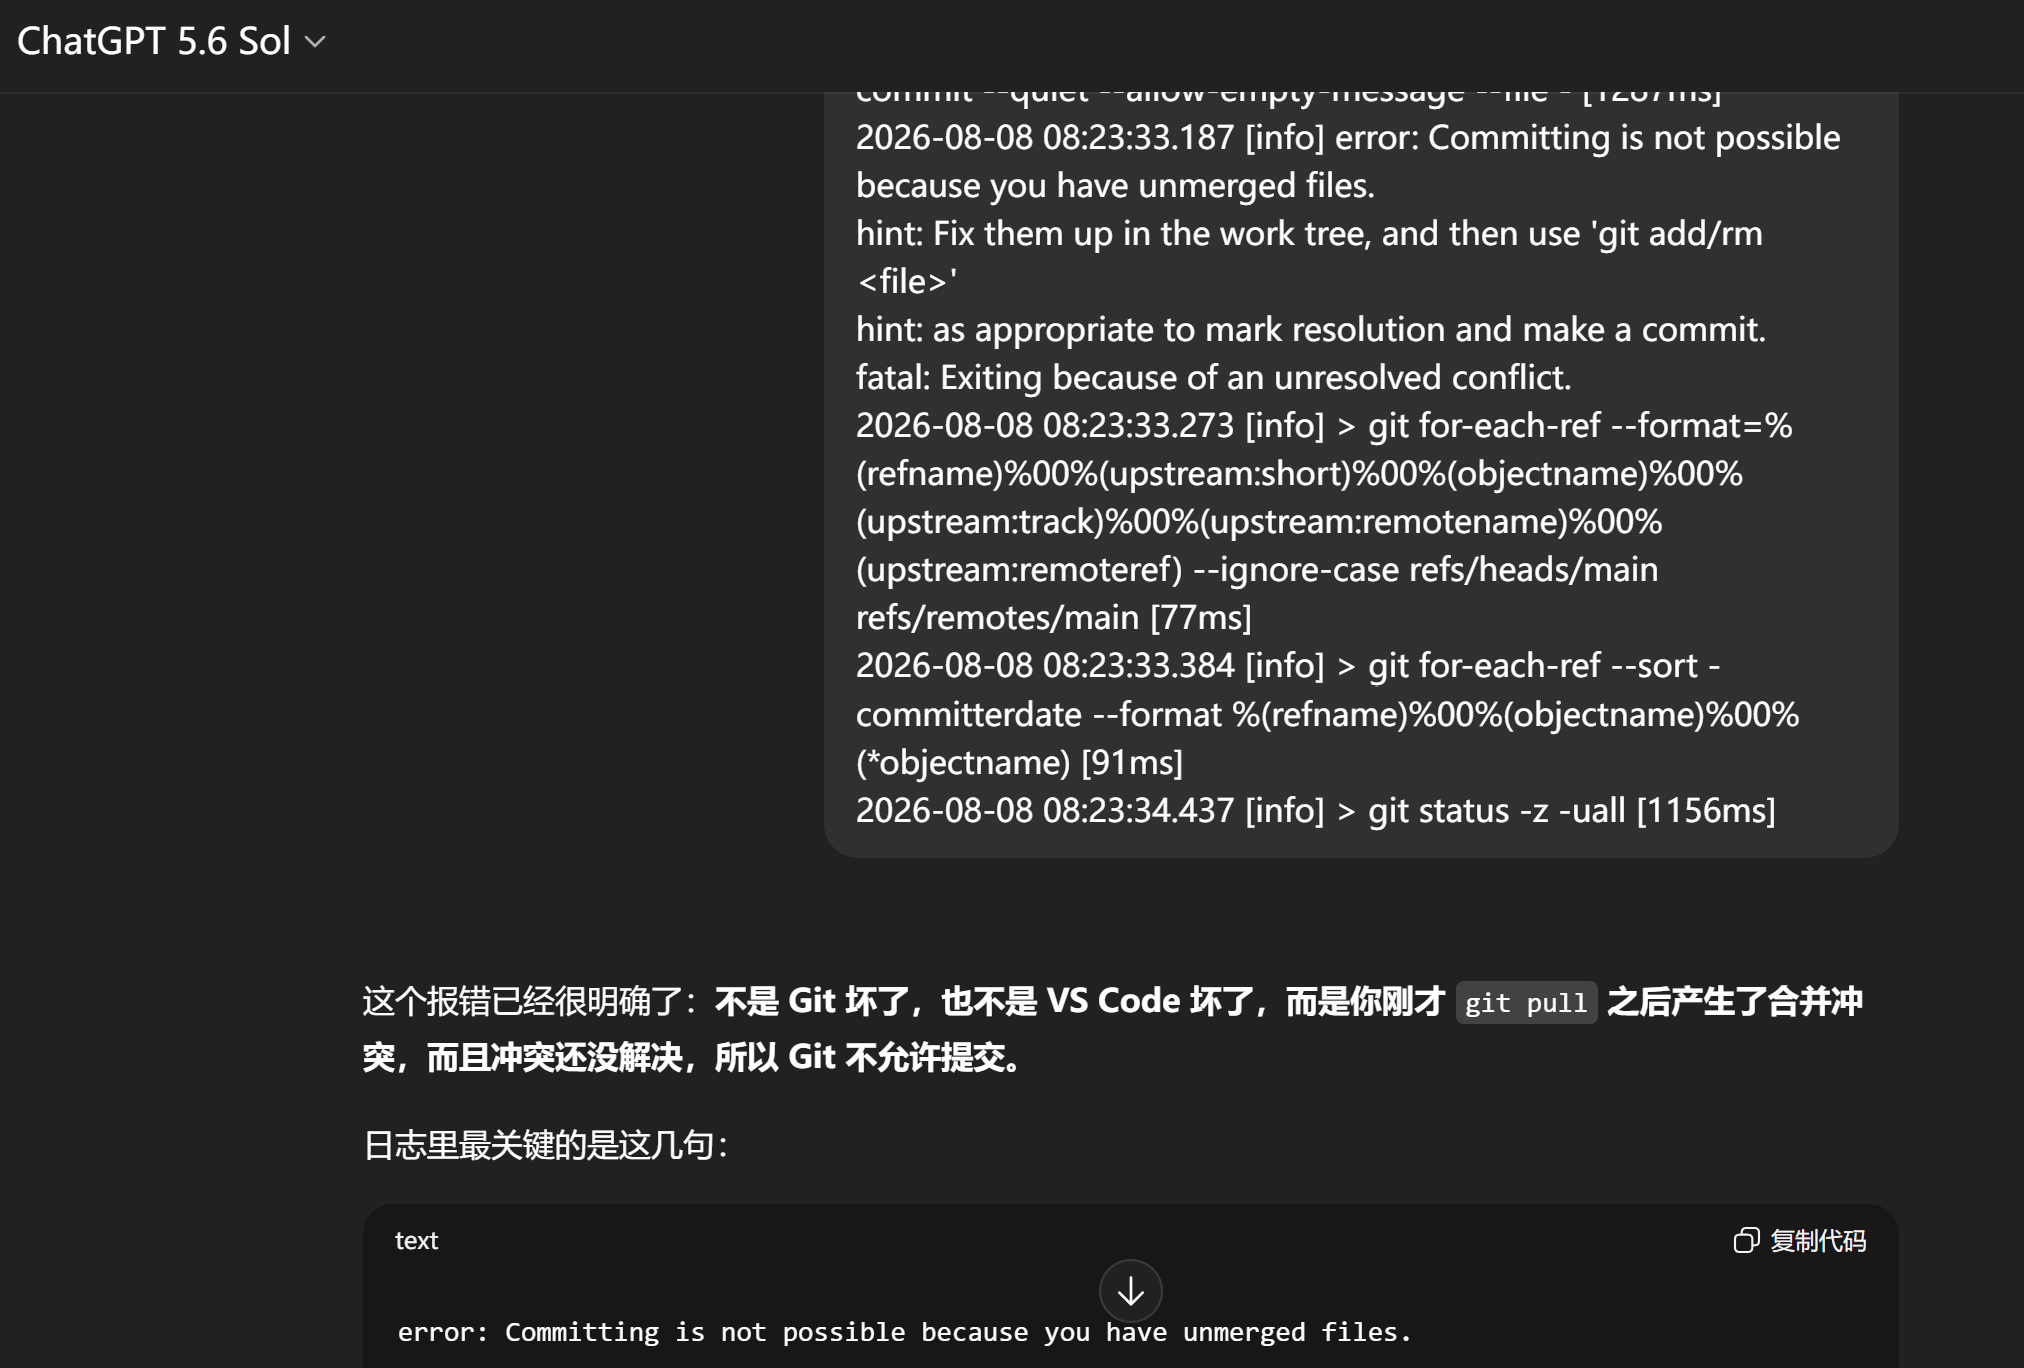
\includegraphics[width=1\textwidth]{figures/人工智能1.png}
\caption{人工智能1}
\end{figure}


\begin{figure}[H]
\centering

\includegraphics[width=1\textwidth]{figures/人工智能2.png}
\caption{人工智能2}
\end{figure}

\end{document}